\mode*
\mode<all>{\topsection{Powierzchnie o stałej krzywiźnie}}

\begin{frame}
Istnieje przykład powierzchni pseudosfery (powstającej przez obrót traktrysy -- krzywej pościgu), o stałej krzywiźnie równej $-1$, jednak ta powierzchnia nie jest zamknięta i nie ma sposobu, aby ją zamknąć nie zaburzając krzywizny.
\pause\begin{center}

\definecolor{c808080}{RGB}{128,128,128}
\usetikzlibrary{arrows}

\mode<presentation>{\begin{tikzpicture}[y=0.80pt, x=0.8pt,yscale=-1,scale=0.3, inner sep=0pt, outer sep=0pt]}
\mode<article>{\begin{tikzpicture}[y=0.80pt, x=0.8pt,yscale=-1,scale=0.4, inner sep=0pt, outer sep=0pt]}
\begin{scope}[shift={(-189.41488,613.09719)}]% layer1
  \begin{scope}% g6915
    \begin{scope}[shift={(-72.90112,-552.22105)}]% g3745
      % path2584-0
      \path[draw=black,line join=miter,line cap=butt,line width=0.800pt,-latex']
        (262.3160,265.0801) -- (718.3477,265.0801);

      % path2582-4
      \path[draw=black,line join=miter,line cap=butt,line width=0.800pt,-latex']
        (352.1790,526.2496) -- (352.7488,-60.8757);

      % path2472
      \path[fill=black] (700.1290,222.7403) .. controls (665.0907,217.3206) and
        (630.0578,211.8397) .. (595.4048,204.3158) .. controls (595.1234,204.2547) and
        (594.8420,204.1934) .. (594.5606,204.1321) .. controls (577.0933,200.3222) and
        (559.7387,195.7575) .. (542.7052,190.2984) .. controls (525.6717,184.8392) and
        (508.9630,178.4882) .. (492.7280,171.0864) .. controls (487.1237,168.5313) and
        (481.5962,165.8047) .. (476.1537,162.9067) .. controls (476.1537,162.9067) and
        (476.1537,162.9067) .. (476.1537,162.9067) .. controls (460.9127,154.7930) and
        (445.8001,146.4437) .. (431.4285,137.0186) .. controls (421.1317,130.2632) and
        (411.2223,122.9167) .. (402.1793,114.6704) .. controls (399.8216,112.5204) and
        (397.5284,110.3021) .. (395.3095,108.0089) .. controls (395.3095,108.0089) and
        (395.3095,108.0089) .. (395.3095,108.0089) .. controls (384.4346,96.7795) and
        (375.4637,83.6984) .. (368.8511,69.4981) .. controls (361.8257,54.4238) and
        (357.3296,38.2303) .. (354.4132,21.7627) .. controls (354.1005,16.8120) and
        (353.0312,14.6437) .. (352.2704,14.8657) .. controls (351.5097,15.0876) and
        (351.0688,17.7450) .. (352.4137,22.3854) .. controls (355.2863,38.9000) and
        (359.7598,55.1916) .. (366.7796,70.4403) .. controls (373.4404,84.8994) and
        (382.5050,98.2369) .. (393.5280,109.7124) .. controls (393.5280,109.7124) and
        (393.5280,109.7124) .. (393.5280,109.7124) .. controls (395.6159,111.8851) and
        (397.7670,113.9913) .. (399.9733,116.0364) .. controls (409.2578,124.6424) and
        (419.4342,132.2758) .. (429.9931,139.2532) .. controls (429.9931,139.2532) and
        (429.9931,139.2532) .. (429.9931,139.2532) .. controls (444.4517,148.8102) and
        (459.6073,157.2536) .. (474.8379,165.4072) .. controls (479.8198,168.0731) and
        (484.8716,170.5951) .. (489.9870,172.9723) .. controls (506.1398,180.4790) and
        (523.6355,186.9800) .. (541.4457,192.4477) .. controls (559.2558,197.9153) and
        (577.3690,202.3713) .. (594.6999,206.1479) .. controls (594.7927,206.1681) and
        (594.8856,206.1883) .. (594.9784,206.2086) .. controls (594.9784,206.2086) and
        (594.9784,206.2086) .. (594.9784,206.2086) .. controls (612.2551,209.9725) and
        (628.7483,213.3371) .. (645.2830,216.4534) .. controls (661.8176,219.5697) and
        (678.3870,222.4138) .. (695.8013,225.0433) .. controls (702.1893,225.9403) and
        (715.4905,227.1505) .. (710.2775,224.7803) .. controls (707.3466,223.8920) and
        (703.5122,223.3002) .. (700.1290,222.7403) -- cycle;

    \end{scope}
    \begin{scope}[shift={(496.59577,-1199.2666)}]% g3730
      % path2884
      \path[fill=black] (322.0428,677.9404) .. controls (320.9074,679.5239) and
        (319.8445,681.1494) .. (318.8381,682.7895) .. controls (314.3244,690.1100) and
        (310.7922,697.9399) .. (307.7306,705.8776) .. controls (307.7306,705.8776) and
        (307.7306,705.8776) .. (307.7306,705.8776) .. controls (303.9031,715.7915) and
        (300.8122,725.9566) .. (298.1392,736.2037) .. controls (298.1392,736.2037) and
        (298.1392,736.2037) .. (298.1392,736.2037) .. controls (291.4112,761.9933) and
        (287.2146,788.3689) .. (284.2992,814.8250) .. controls (280.7817,846.7296) and
        (279.2578,878.8481) .. (279.3487,910.9528) .. controls (279.3638,916.3125) and
        (279.4239,921.6728) .. (279.5314,927.0325) .. controls (280.0670,953.7556) and
        (281.6703,980.4662) .. (284.6386,1007.0428) .. controls (284.6386,1007.0428)
        and (284.6386,1007.0428) .. (284.6386,1007.0428) .. controls
        (287.5891,1033.4690) and (291.7982,1059.8267) .. (298.5908,1085.5824) ..
        controls (298.5908,1085.5824) and (298.5908,1085.5824) .. (298.5908,1085.5824)
        .. controls (301.2875,1095.8078) and (304.4075,1105.9449) ..
        (308.2718,1115.8159) .. controls (308.2718,1115.8159) and (308.2718,1115.8159)
        .. (308.2718,1115.8159) .. controls (311.3630,1123.7172) and
        (314.9226,1131.4939) .. (319.4547,1138.7298) .. controls (319.4547,1138.7298)
        and (319.4547,1138.7298) .. (319.4547,1138.7298) .. controls
        (322.8414,1144.1529) and (326.8243,1149.3801) .. (331.9780,1153.3672) ..
        controls (334.0238,1154.9479) and (336.2810,1156.3049) .. (338.7358,1157.2460)
        .. controls (340.9753,1158.1030) and (343.3724,1158.5800) ..
        (345.7907,1158.5789) .. controls (347.5191,1158.5789) and (349.2356,1158.3269)
        .. (350.8905,1157.8701) .. controls (351.5468,1157.6889) and
        (352.1935,1157.4750) .. (352.8275,1157.2304) .. controls (355.2678,1156.2870)
        and (357.5096,1154.9301) .. (359.5401,1153.3503) .. controls
        (364.6502,1149.3692) and (368.5882,1144.1563) .. (371.9378,1138.7511) ..
        controls (376.4226,1131.5346) and (379.9439,1123.7842) .. (383.0082,1115.9124)
        .. controls (386.8424,1106.0687) and (389.9480,1095.9628) ..
        (392.6413,1085.7698) .. controls (392.6413,1085.7698) and (392.6413,1085.7698)
        .. (392.6413,1085.7698) .. controls (399.4337,1060.0645) and
        (403.7103,1033.7533) .. (406.6940,1007.3657) .. controls (406.6940,1007.3657)
        and (406.6940,1007.3657) .. (406.6940,1007.3657) .. controls
        (410.0922,977.3269) and (411.6989,947.0970) .. (411.7924,916.8841) .. controls
        (411.7984,915.0105) and (411.7984,913.1371) .. (411.7944,911.2637) .. controls
        (411.7151,879.1349) and (410.1081,846.9997) .. (406.5252,815.0836) .. controls
        (403.5558,788.6203) and (399.3172,762.2381) .. (392.5255,736.4780) .. controls
        (392.5255,736.4780) and (392.5255,736.4780) .. (392.5255,736.4780) .. controls
        (389.8291,726.2503) and (386.7142,716.1137) .. (382.8623,706.2480) .. controls
        (382.8623,706.2480) and (382.8623,706.2480) .. (382.8623,706.2480) .. controls
        (379.7824,698.3556) and (376.2416,690.5920) .. (371.7363,683.3789) .. controls
        (368.8376,678.7279) and (365.5099,674.2285) .. (361.3882,670.5566) .. controls
        (360.7249,669.9081) and (360.0603,669.3124) .. (359.3997,668.7669) .. controls
        (357.0555,666.8334) and (354.7365,665.6000) .. (352.7435,664.9062) .. controls
        (350.4678,664.1152) and (348.6502,664.0151) .. (347.4822,664.1087) .. controls
        (346.3141,664.2023) and (345.7718,664.4776) .. (345.7916,664.7238) .. controls
        (345.8113,664.9700) and (346.3855,665.1926) .. (347.4340,665.5058) .. controls
        (348.4826,665.8191) and (350.0169,666.2347) .. (351.9152,667.0550) .. controls
        (353.6610,667.8068) and (355.7165,668.9323) .. (357.9870,670.5805) .. controls
        (358.8001,671.1698) and (359.6367,671.8202) .. (360.4936,672.5387) .. controls
        (364.1761,675.9429) and (367.2197,680.1220) .. (369.9484,684.4835) .. controls
        (374.3496,691.5451) and (377.8187,699.1965) .. (380.8614,707.0184) .. controls
        (380.8614,707.0184) and (380.8614,707.0184) .. (380.8614,707.0184) .. controls
        (384.6601,716.7911) and (387.7326,726.8541) .. (390.3983,737.0292) .. controls
        (390.3983,737.0292) and (390.3983,737.0292) .. (390.3983,737.0292) .. controls
        (397.1129,762.6605) and (401.2865,788.9412) .. (404.2060,815.3361) .. controls
        (407.7253,847.1639) and (409.2734,879.2145) .. (409.3011,911.2637) .. controls
        (409.3021,912.5856) and (409.3007,913.9075) .. (409.2971,915.2294) .. controls
        (409.2023,945.9148) and (407.5496,976.6046) .. (404.0507,1007.0772) ..
        controls (401.0297,1033.3780) and (396.7367,1059.5537) .. (389.9541,1085.0709)
        .. controls (387.2646,1095.1882) and (384.1795,1105.1889) ..
        (380.3832,1114.8971) .. controls (380.3832,1114.8972) and (380.3832,1114.8972)
        .. (380.3832,1114.8972) .. controls (377.3419,1122.6661) and
        (373.8908,1130.2559) .. (369.5248,1137.2529) .. controls (369.5248,1137.2529)
        and (369.5248,1137.2529) .. (369.5248,1137.2529) .. controls
        (366.2376,1142.4932) and (362.5200,1147.4531) .. (357.7907,1151.0918) ..
        controls (356.4460,1152.1290) and (355.0294,1153.0526) .. (353.5458,1153.7910)
        .. controls (352.9752,1154.0750) and (352.3943,1154.3317) ..
        (351.8033,1154.5570) .. controls (351.8033,1154.5570) and (351.8033,1154.5570)
        .. (351.8033,1154.5570) .. controls (349.8773,1155.2943) and
        (347.8284,1155.7122) .. (345.7915,1155.7106) .. controls (345.7915,1155.7106)
        and (345.7915,1155.7106) .. (345.7915,1155.7106) .. controls
        (343.7612,1155.7206) and (341.7062,1155.3050) .. (339.7630,1154.5670) ..
        controls (337.6286,1153.7594) and (335.6122,1152.5411) .. (333.7294,1151.0997)
        .. controls (333.7294,1151.0997) and (333.7294,1151.0997) ..
        (333.7294,1151.0997) .. controls (328.9795,1147.4720) and (325.2037,1142.5063)
        .. (321.8554,1137.2259) .. controls (317.4547,1130.2510) and
        (313.9380,1122.6403) .. (310.8322,1114.8117) .. controls (310.8322,1114.8117)
        and (310.8322,1114.8117) .. (310.8322,1114.8117) .. controls
        (306.9932,1105.1250) and (303.8491,1095.0931) .. (301.1063,1084.9159) ..
        controls (294.2259,1059.3845) and (289.8513,1033.0219) .. (286.7891,1006.8018)
        .. controls (283.5908,979.4057) and (281.9305,952.1293) .. (281.4455,925.6243)
        .. controls (281.3555,920.7081) and (281.3095,915.8183) .. (281.3038,910.9528)
        .. controls (281.2662,878.1442) and (283.0424,846.4333) .. (286.7098,815.0951)
        .. controls (289.7834,788.8398) and (294.0708,762.8037) .. (300.9203,736.9406)
        .. controls (303.5901,726.8604) and (306.6568,716.8171) .. (310.4745,706.9537)
        .. controls (313.0675,700.2598) and (315.9763,693.6374) .. (319.5537,687.3407)
        .. controls (320.0852,686.3955) and (320.6688,685.3850) .. (321.3015,684.3327)
        .. controls (322.7735,681.8920) and (324.5003,679.2111) .. (326.4617,676.6714)
        .. controls (328.4231,674.1317) and (330.6296,671.7482) .. (332.9440,669.7887)
        .. controls (335.0171,668.0322) and (337.1760,666.6563) .. (339.1492,665.7365)
        .. controls (342.1018,664.3598) and (344.5751,664.0037) .. (345.4463,663.7057)
        .. controls (345.8819,663.5567) and (345.9265,663.4102) .. (345.4581,663.2685)
        .. controls (344.9897,663.1268) and (344.0011,662.9820) .. (342.4070,663.1019)
        .. controls (341.1296,663.2665) and (339.8100,663.5765) .. (338.4989,664.0394)
        .. controls (336.0583,664.9037) and (333.6692,666.2588) .. (331.4998,667.9180)
        .. controls (327.7976,670.7547) and (324.6339,674.3600) .. (322.0428,677.9404)
        -- cycle;

      % path2886
      \path[fill=c808080] (399.7575,1054.3284) .. controls (400.1346,1052.2232) and
        (400.4980,1050.1155) .. (400.8482,1048.0055) .. controls (401.5487,1043.7857)
        and (402.1966,1039.5569) .. (402.7958,1035.3212) .. controls
        (404.1259,1025.9190) and (405.6795,1016.4924) .. (406.6994,1007.0578) ..
        controls (410.1493,975.1574) and (412.1310,943.0539) .. (412.0176,910.9529) --
        (412.0176,910.9529) .. controls (412.0176,910.0885) and (412.0076,909.2241) ..
        (412.0046,908.3597) .. controls (411.7951,877.1313) and (410.3465,845.8645) ..
        (407.1786,814.7632) .. controls (406.0402,803.5785) and (404.6305,792.4059) ..
        (402.8054,781.3009) .. controls (402.1817,777.5062) and (401.5201,773.7178) ..
        (400.8167,769.9375) .. controls (402.5169,767.3734) and (396.1837,759.7347) ..
        (396.8069,764.3123) .. controls (397.1659,766.1550) and (397.5144,768.0000) ..
        (397.8528,769.8472) .. controls (398.5297,773.5416) and (399.1665,777.2443) ..
        (399.7669,780.9540) .. controls (401.5994,792.2767) and (402.9955,803.6774) ..
        (404.1129,815.0972) .. controls (407.0795,845.4302) and (408.4408,875.9157) ..
        (408.6236,906.3679) .. controls (408.6336,907.8911) and (408.6396,909.4194) ..
        (408.6436,910.9526) .. controls (408.6836,926.4880) and (408.4473,942.5182) ..
        (407.7911,958.6310) .. controls (407.1349,974.7438) and (405.8561,990.9387) ..
        (404.2920,1006.7950) .. controls (403.3262,1016.5812) and (401.7914,1026.2424)
        .. (400.4420,1035.6623) .. controls (399.8284,1039.9458) and
        (399.1580,1044.1771) .. (398.4304,1048.3630) .. controls (398.0666,1050.4559)
        and (397.6885,1052.5375) .. (397.2961,1054.6086) .. controls
        (396.9036,1056.6798) and (399.3805,1056.4336) .. (399.7575,1054.3284) --
        cycle;

      \begin{scope}[cm={{0.0,-0.63723,-1.0,0.0,(1950.1599,-1100.1531)}}]% g2686
        % path3602-6
        \path[fill=c808080] (-3007.4113,1470.5202) .. controls (-3008.0967,1470.1240)
          and (-3008.7867,1469.7471) .. (-3009.4766,1469.3860) .. controls
          (-3014.3022,1466.8308) and (-3019.3615,1464.8808) .. (-3024.4435,1463.2019) ..
          controls (-3024.4435,1463.2019) and (-3024.4435,1463.2019) ..
          (-3024.4435,1463.2019) .. controls (-3030.8725,1461.0739) and
          (-3037.4122,1459.3727) .. (-3043.9796,1457.9048) .. controls
          (-3043.9796,1457.9048) and (-3043.9796,1457.9048) .. (-3043.9796,1457.9048) ..
          controls (-3060.6314,1454.1822) and (-3077.5458,1451.8789) ..
          (-3094.4855,1450.2813) .. controls (-3114.9858,1448.3465) and
          (-3135.5859,1447.5223) .. (-3156.1745,1447.6306) .. controls
          (-3159.5978,1447.6486) and (-3163.0214,1447.6926) .. (-3166.4447,1447.7631) ..
          controls (-3183.5954,1448.1186) and (-3200.7399,1449.0264) ..
          (-3217.8243,1450.6838) .. controls (-3217.8243,1450.6838) and
          (-3217.8243,1450.6838) .. (-3217.8243,1450.6838) .. controls
          (-3234.7389,1452.3237) and (-3251.6345,1454.6446) .. (-3268.2439,1458.4478) ..
          controls (-3268.2439,1458.4478) and (-3268.2439,1458.4478) ..
          (-3268.2439,1458.4478) .. controls (-3274.7891,1459.9463) and
          (-3281.2986,1461.6855) .. (-3287.6797,1463.8615) .. controls
          (-3287.6797,1463.8615) and (-3287.6797,1463.8616) .. (-3287.6797,1463.8616) ..
          controls (-3292.7234,1465.5794) and (-3297.7241,1467.5672) ..
          (-3302.4534,1470.1522) .. controls (-3305.8915,1472.0187) and
          (-3309.2884,1474.2476) .. (-3311.9926,1477.2914) .. controls
          (-3313.0216,1478.4506) and (-3313.9334,1479.7668) .. (-3314.5860,1481.2473) ..
          controls (-3315.1641,1482.5628) and (-3315.4948,1484.0048) ..
          (-3315.4959,1485.4786) .. controls (-3315.4859,1486.7341) and
          (-3315.2427,1487.9640) .. (-3314.8093,1489.1107) .. controls
          (-3314.7343,1489.3102) and (-3314.6528,1489.5072) .. (-3314.5664,1489.7013) ..
          controls (-3313.9079,1491.1761) and (-3312.9928,1492.4853) ..
          (-3311.9622,1493.6389) .. controls (-3309.2534,1496.6687) and
          (-3305.8611,1498.8885) .. (-3302.4274,1500.7576) .. controls
          (-3297.7047,1503.3449) and (-3292.7141,1505.3500) .. (-3287.6800,1507.0965) ..
          controls (-3281.3115,1509.3086) and (-3274.8143,1511.1018) ..
          (-3268.2795,1512.6634) .. controls (-3251.6994,1516.6258) and
          (-3234.8121,1519.1677) .. (-3217.8904,1520.9499) .. controls
          (-3217.8904,1520.9499) and (-3217.8904,1520.9499) .. (-3217.8904,1520.9499) ..
          controls (-3198.5989,1522.9834) and (-3179.2006,1523.9632) ..
          (-3159.8169,1523.9729) .. controls (-3158.6027,1523.9735) and
          (-3157.3885,1523.9729) .. (-3156.1745,1523.9629) .. controls
          (-3135.5707,1523.8679) and (-3114.9646,1522.8820) .. (-3094.4781,1520.7484) ..
          controls (-3077.5542,1518.9872) and (-3060.6651,1516.4938) ..
          (-3044.1016,1512.5225) .. controls (-3044.1016,1512.5225) and
          (-3044.1016,1512.5225) .. (-3044.1016,1512.5225) .. controls
          (-3037.5703,1510.9567) and (-3031.0809,1509.1506) .. (-3024.7308,1506.9137) ..
          controls (-3024.7307,1506.9137) and (-3024.7307,1506.9137) ..
          (-3024.7307,1506.9137) .. controls (-3019.7096,1505.1467) and
          (-3014.7409,1503.1153) .. (-3010.0612,1500.4999) .. controls
          (-3007.3931,1499.0160) and (-3004.7622,1497.3234) .. (-3002.4871,1495.2123) ..
          controls (-3001.7646,1494.6482) and (-3001.1250,1494.0652) ..
          (-3000.5653,1493.4785) .. controls (-2999.3078,1492.1591) and
          (-2998.4982,1490.7760) .. (-2998.0739,1489.5709) .. controls
          (-2997.6023,1488.2293) and (-2997.6137,1487.1378) .. (-2997.7712,1486.4518) ..
          controls (-2997.9287,1485.7657) and (-2998.2219,1485.4662) ..
          (-2998.4955,1485.4764) .. controls (-2998.7692,1485.4864) and
          (-2999.0290,1485.7963) .. (-2999.3260,1486.3217) .. controls
          (-2999.6230,1486.8471) and (-2999.9667,1487.5936) .. (-3000.4888,1488.5107) ..
          controls (-3000.9825,1489.3850) and (-3001.6754,1490.4184) ..
          (-3002.6488,1491.6355) .. controls (-3003.1655,1492.2818) and
          (-3003.7526,1492.9646) .. (-3004.4246,1493.6846) .. controls
          (-3006.4292,1495.4692) and (-3008.7940,1496.9578) .. (-3011.2456,1498.3341) ..
          controls (-3015.7542,1500.8433) and (-3020.5989,1502.8019) ..
          (-3025.5464,1504.5315) .. controls (-3025.5464,1504.5315) and
          (-3025.5464,1504.5315) .. (-3025.5464,1504.5315) .. controls
          (-3031.7963,1506.7134) and (-3038.2071,1508.4751) .. (-3044.6833,1510.0079) ..
          controls (-3044.6833,1510.0079) and (-3044.6833,1510.0079) ..
          (-3044.6833,1510.0079) .. controls (-3061.1107,1513.8955) and
          (-3077.8926,1516.3164) .. (-3094.7451,1518.0197) .. controls
          (-3115.1382,1520.0797) and (-3135.6546,1520.9969) .. (-3156.1745,1521.0298) ..
          controls (-3157.0380,1521.0298) and (-3157.9015,1521.0298) ..
          (-3158.7650,1521.0292) .. controls (-3178.4150,1520.9882) and
          (-3198.0651,1519.9499) .. (-3217.5855,1517.8308) .. controls
          (-3234.4157,1516.0028) and (-3251.1601,1513.4358) .. (-3267.5423,1509.4742) ..
          controls (-3273.9978,1507.9129) and (-3280.3830,1506.1362) ..
          (-3286.6061,1503.9577) .. controls (-3286.6061,1503.9577) and
          (-3286.6061,1503.9577) .. (-3286.6061,1503.9577) .. controls
          (-3291.5328,1502.2295) and (-3296.3468,1500.2914) .. (-3300.8225,1497.8205) ..
          controls (-3300.8225,1497.8205) and (-3300.8225,1497.8205) ..
          (-3300.8225,1497.8205) .. controls (-3304.0850,1495.9975) and
          (-3307.1732,1494.0122) .. (-3309.4433,1491.4082) .. controls
          (-3309.9092,1490.8746) and (-3310.3382,1490.3271) .. (-3310.7071,1489.7642) ..
          controls (-3311.0098,1489.3022) and (-3311.2723,1488.8292) ..
          (-3311.4812,1488.3444) .. controls (-3311.4812,1488.3444) and
          (-3311.4812,1488.3443) .. (-3311.4812,1488.3443) .. controls
          (-3311.8852,1487.4142) and (-3312.1271,1486.4273) .. (-3312.1213,1485.4761) ..
          controls (-3312.1213,1485.4761) and (-3312.1213,1485.4761) ..
          (-3312.1213,1485.4761) .. controls (-3312.1323,1484.5288) and
          (-3311.8971,1483.5394) .. (-3311.4954,1482.6016) .. controls
          (-3311.0382,1481.5259) and (-3310.3159,1480.5018) .. (-3309.4675,1479.5225) ..
          controls (-3309.4675,1479.5225) and (-3309.4675,1479.5225) ..
          (-3309.4675,1479.5225) .. controls (-3307.2147,1476.9185) and
          (-3304.1301,1474.9155) .. (-3300.8521,1473.0774) .. controls
          (-3296.4000,1470.6100) and (-3291.5821,1468.6629) .. (-3286.6288,1466.9284) ..
          controls (-3286.6288,1466.9284) and (-3286.6288,1466.9284) ..
          (-3286.6288,1466.9284) .. controls (-3280.4288,1464.7614) and
          (-3274.0338,1462.9907) .. (-3267.5514,1461.4387) .. controls
          (-3251.1749,1457.5185) and (-3234.3302,1455.0056) .. (-3217.5758,1453.2207) ..
          controls (-3200.0046,1451.3501) and (-3182.5240,1450.3472) ..
          (-3165.5422,1450.0254) .. controls (-3162.4031,1449.9664) and
          (-3159.2810,1449.9344) .. (-3156.1745,1449.9274) .. controls
          (-3135.1565,1449.8834) and (-3114.8549,1450.9805) .. (-3094.7644,1453.1293) ..
          controls (-3077.9993,1454.9235) and (-3061.3694,1457.3781) ..
          (-3044.7443,1461.2081) .. controls (-3038.3188,1462.6885) and
          (-3031.9053,1464.3757) .. (-3025.5670,1466.4806) .. controls
          (-3021.7314,1467.7565) and (-3017.9252,1469.1636) .. (-3014.2439,1470.8691) ..
          controls (-3013.2857,1471.3035) and (-3012.2204,1471.8003) ..
          (-3011.1018,1472.3549) .. controls (-3009.4945,1473.1580) and
          (-3007.7706,1474.0621) .. (-3006.1408,1475.0837) .. controls
          (-3004.5110,1476.1053) and (-3002.9828,1477.2521) .. (-3001.6917,1478.4700) ..
          controls (-3000.5431,1479.5525) and (-2999.6085,1480.6910) ..
          (-2998.9467,1481.7643) .. controls (-2997.9455,1483.3877) and
          (-2997.5876,1484.8323) .. (-2997.2586,1485.3086) .. controls
          (-2997.0942,1485.5468) and (-2996.9256,1485.5459) .. (-2996.7650,1485.2080) ..
          controls (-2996.6044,1484.8701) and (-2996.4460,1484.1871) ..
          (-2996.5057,1483.1072) .. controls (-2996.6096,1482.3900) and
          (-2996.7980,1481.6591) .. (-2997.0723,1480.9415) .. controls
          (-2997.6603,1479.4095) and (-2998.5777,1477.9542) .. (-2999.6749,1476.6859) ..
          controls (-3001.8845,1474.1370) and (-3004.7172,1472.1065) ..
          (-3007.4113,1470.5202) -- cycle;

        % path3604-9
        \path[fill=black] (-3312.2875,1494.6965) .. controls (-3309.4619,1497.5671) and
          (-3306.1136,1499.6469) .. (-3302.7656,1501.3759) .. controls
          (-3302.7656,1501.3759) and (-3302.7656,1501.3759) .. (-3302.7656,1501.3759) ..
          controls (-3297.9412,1503.8941) and (-3292.8922,1505.8236) ..
          (-3287.8166,1507.4952) .. controls (-3287.8166,1507.4952) and
          (-3287.8166,1507.4952) .. (-3287.8166,1507.4952) .. controls
          (-3281.3979,1509.6128) and (-3274.8698,1511.3190) .. (-3268.3089,1512.7904) ..
          controls (-3268.3089,1512.7904) and (-3268.3089,1512.7904) ..
          (-3268.3089,1512.7904) .. controls (-3257.3463,1515.2494) and
          (-3246.2618,1517.0846) .. (-3235.1200,1518.4164) .. controls
          (-3229.3601,1519.1049) and (-3223.5931,1519.7186) .. (-3217.8242,1520.2729) ..
          controls (-3197.3418,1522.2417) and (-3176.7590,1523.3813) ..
          (-3156.1745,1523.2668) .. controls (-3156.1745,1523.2668) and
          (-3156.1745,1523.2668) .. (-3156.1745,1523.2668) .. controls
          (-3155.6262,1523.2668) and (-3155.0780,1523.2568) .. (-3154.5297,1523.2548) ..
          controls (-3134.4989,1523.0783) and (-3114.4357,1522.7970) ..
          (-3094.4480,1521.0584) .. controls (-3087.5640,1520.4603) and
          (-3080.6841,1519.6976) .. (-3073.8402,1518.6760) .. controls
          (-3063.8216,1517.1804) and (-3053.8568,1515.3112) .. (-3044.0129,1512.9084) ..
          controls (-3037.4781,1511.3135) and (-3030.9849,1509.4715) ..
          (-3024.6361,1507.1925) .. controls (-3019.6157,1505.3925) and
          (-3014.6464,1503.3203) .. (-3009.9738,1500.6618) .. controls
          (-3009.9738,1500.6618) and (-3009.9738,1500.6618) .. (-3009.9738,1500.6618) ..
          controls (-3006.5752,1498.7391) and (-3003.2356,1496.4649) ..
          (-3000.6311,1493.4227) .. controls (-3000.6311,1493.4227) and
          (-3000.6311,1493.4227) .. (-3000.6311,1493.4226) .. controls
          (-2999.9821,1492.6643) and (-2999.3857,1491.8453) .. (-2998.8820,1490.9660) ..
          controls (-2998.5133,1490.5144) and (-2998.2202,1490.0547) ..
          (-2997.9959,1489.6075) .. controls (-2997.3519,1488.3192) and
          (-2997.3195,1487.1792) .. (-2997.5168,1486.4716) .. controls
          (-2997.7141,1485.7641) and (-2998.1222,1485.4645) .. (-2998.5093,1485.4789) ..
          controls (-2998.8964,1485.4929) and (-2999.2695,1485.7990) ..
          (-2999.6024,1486.3004) .. controls (-2999.9353,1486.8019) and
          (-3000.2294,1487.5011) .. (-3000.5737,1488.4758) .. controls
          (-3000.7182,1488.8870) and (-3000.8794,1489.3491) .. (-3001.0704,1489.8759) ..
          controls (-3001.4705,1490.5386) and (-3001.9483,1491.1777) ..
          (-3002.4723,1491.7939) .. controls (-3002.4723,1491.7939) and
          (-3002.4723,1491.7939) .. (-3002.4723,1491.7939) .. controls
          (-3004.7771,1494.5065) and (-3007.9049,1496.5796) .. (-3011.1879,1498.4420) ..
          controls (-3011.1879,1498.4420) and (-3011.1879,1498.4420) ..
          (-3011.1879,1498.4420) .. controls (-3015.6928,1500.9773) and
          (-3020.5395,1502.9585) .. (-3025.4881,1504.7041) .. controls
          (-3031.7389,1506.9065) and (-3038.1541,1508.6819) .. (-3044.6342,1510.2224) ..
          controls (-3054.2310,1512.5036) and (-3063.9519,1514.2734) ..
          (-3073.7357,1515.6860) .. controls (-3080.7073,1516.6925) and
          (-3087.7225,1517.4270) .. (-3094.7479,1517.9934) .. controls
          (-3114.2196,1519.5620) and (-3133.7590,1519.7538) .. (-3153.2704,1519.8769) ..
          controls (-3154.2352,1519.8869) and (-3155.2033,1519.8879) ..
          (-3156.1745,1519.8919) .. controls (-3166.1237,1519.9319) and
          (-3176.3929,1519.8529) .. (-3186.7182,1519.5456) .. controls
          (-3197.0435,1519.2381) and (-3207.4248,1518.7007) .. (-3217.5893,1517.8716) ..
          controls (-3223.5725,1517.3831) and (-3229.4815,1516.8024) ..
          (-3235.2523,1516.1010) .. controls (-3246.5154,1514.7320) and
          (-3257.2141,1512.6790) .. (-3267.6767,1510.0574) .. controls
          (-3274.1312,1508.4400) and (-3280.4864,1506.6055) .. (-3286.7576,1504.4024) ..
          controls (-3291.6476,1502.6819) and (-3296.4823,1500.7779) ..
          (-3301.1042,1498.3378) .. controls (-3303.4215,1497.1032) and
          (-3305.6970,1495.7802) .. (-3307.7248,1494.1790) .. controls
          (-3308.4672,1493.6130) and (-3309.3544,1492.9113) .. (-3310.2325,1492.1085) ..
          controls (-3311.2641,1491.1673) and (-3312.2584,1490.0923) ..
          (-3313.0044,1489.0153) .. controls (-3313.4353,1488.3947) and
          (-3313.7889,1487.7742) .. (-3314.0779,1487.2273) .. controls
          (-3314.3668,1486.6805) and (-3314.5934,1486.2068) .. (-3314.8057,1485.8893) ..
          controls (-3315.0180,1485.5718) and (-3315.2218,1485.4100) ..
          (-3315.4384,1485.5055) .. controls (-3315.6551,1485.6005) and
          (-3315.8919,1485.9572) .. (-3316.0431,1486.6767) .. controls
          (-3316.0851,1487.7505) and (-3315.8713,1488.9415) .. (-3315.4175,1490.0746) ..
          controls (-3314.7789,1491.6614) and (-3313.7539,1493.1029) ..
          (-3312.6817,1494.2751) .. controls (-3312.5505,1494.4185) and
          (-3312.4189,1494.5589) .. (-3312.2875,1494.6965) -- cycle;

      \end{scope}
      % path2692
      \path[fill=c808080] (592.2498,857.0247) .. controls (592.4832,857.3307) and
        (592.7118,857.6529) .. (592.9382,857.9849) .. controls (592.9382,857.9849) and
        (592.9382,857.9849) .. (592.9382,857.9849) .. controls (595.2881,861.4924) and
        (596.6972,865.7177) .. (597.9179,870.0310) .. controls (597.9179,870.0310) and
        (597.9179,870.0310) .. (597.9179,870.0310) .. controls (601.6402,883.3181) and
        (602.6178,897.3359) .. (602.7931,911.2936) .. controls (602.7931,911.2936) and
        (602.7931,911.2936) .. (602.7931,911.2936) .. controls (602.8082,912.5785) and
        (602.8166,913.8642) .. (602.8172,915.1502) .. controls (602.8242,927.8179) and
        (601.6358,940.5101) .. (598.3816,952.6775) .. controls (597.2122,957.0181) and
        (595.8679,961.3035) .. (593.5729,964.9948) .. controls (593.5729,964.9948) and
        (593.5729,964.9948) .. (593.5729,964.9948) .. controls (592.8075,966.2133) and
        (591.9777,967.3470) .. (590.9397,968.1505) .. controls (590.1762,968.7273) and
        (589.3148,969.1574) .. (588.4961,969.1359) .. controls (588.1968,969.1490) and
        (587.8902,969.1017) .. (587.5836,969.0085) .. controls (587.0513,968.8467) and
        (586.5197,968.5446) .. (586.0293,968.1799) .. controls (584.9797,967.3806) and
        (584.1427,966.2425) .. (583.3802,965.0190) .. controls (581.0939,961.3136) and
        (579.8252,957.0018) .. (578.7535,952.6401) .. controls (578.7535,952.6401) and
        (578.7535,952.6401) .. (578.7535,952.6401) .. controls (575.5838,939.6189) and
        (574.9847,926.1216) .. (574.7731,912.6569) .. controls (574.7661,912.2025) and
        (574.7598,911.7481) .. (574.7547,911.2937) .. controls (574.7547,911.2937) and
        (574.7547,911.2937) .. (574.7547,911.2937) .. controls (574.6138,897.3651) and
        (575.3743,883.3862) .. (578.6347,869.9161) .. controls (578.6347,869.9161) and
        (578.6347,869.9161) .. (578.6347,869.9161) .. controls (579.7009,865.5478) and
        (580.9389,861.2249) .. (583.1721,857.4396) .. controls (583.1721,857.4396) and
        (583.1721,857.4396) .. (583.1721,857.4396) .. controls (583.8085,856.3691) and
        (584.5061,855.3503) .. (585.3642,854.5321) .. controls (585.5474,854.4211) and
        (585.7205,854.3184) .. (585.8846,854.2222) .. controls (586.7850,853.7076) and
        (587.3784,853.3715) .. (587.8048,853.0411) .. controls (588.2312,852.7108) and
        (588.5114,852.3698) .. (588.4955,852.0064) .. controls (588.4795,851.6430) and
        (588.1118,851.2551) .. (587.3411,851.1796) .. controls (586.9557,851.1419) and
        (586.4776,851.1886) .. (585.9655,851.3732) .. controls (585.4534,851.5575) and
        (584.9089,851.8822) .. (584.4305,852.3637) .. controls (584.2116,852.5806) and
        (584.0007,852.8245) .. (583.8042,853.0948) .. controls (582.7926,854.0743) and
        (582.0002,855.1896) .. (581.3428,856.3084) .. controls (581.3428,856.3084) and
        (581.3428,856.3084) .. (581.3428,856.3084) .. controls (578.9116,860.3972) and
        (577.5541,864.9131) .. (576.4590,869.3470) .. controls (576.4590,869.3470) and
        (576.4590,869.3470) .. (576.4590,869.3470) .. controls (573.0400,883.0670) and
        (572.1470,897.2478) .. (572.2029,911.2937) .. controls (572.2029,911.2937) and
        (572.2029,911.2937) .. (572.2029,911.2937) .. controls (572.2039,911.6209) and
        (572.2059,911.9482) .. (572.2079,912.2756) .. controls (572.2528,919.1335) and
        (572.4017,926.0212) .. (572.9388,932.8888) .. controls (573.4759,939.7563) and
        (574.4027,946.6072) .. (576.0032,953.3595) .. controls (576.0032,953.3595) and
        (576.0032,953.3595) .. (576.0032,953.3595) .. controls (577.0469,957.8212) and
        (578.4055,962.4004) .. (580.9068,966.5485) .. controls (580.9068,966.5485) and
        (580.9068,966.5485) .. (580.9068,966.5485) .. controls (581.7312,967.9379) and
        (582.7912,969.3336) .. (584.2272,970.4836) .. controls (584.6173,970.8044) and
        (585.0525,971.0905) .. (585.5263,971.3283) .. controls (586.3969,971.7653) and
        (587.4003,972.0420) .. (588.4962,972.0718) .. controls (590.1734,972.0157) and
        (591.6414,971.3795) .. (592.7464,970.4596) .. controls (592.7464,970.4596) and
        (592.7464,970.4596) .. (592.7464,970.4596) .. controls (594.1639,969.3098) and
        (595.2157,967.9149) .. (596.0385,966.5194) .. controls (596.0385,966.5194) and
        (596.0385,966.5194) .. (596.0385,966.5194) .. controls (598.4974,962.4136) and
        (599.8823,957.8381) .. (600.9577,953.3513) .. controls (602.5077,946.9656) and
        (603.4815,940.4474) .. (604.0560,933.9734) .. controls (604.6304,927.4994) and
        (604.8097,921.0699) .. (604.8046,914.8474) .. controls (604.8037,913.6554) and
        (604.7996,912.4711) .. (604.7938,911.2937) .. controls (604.7938,911.2937) and
        (604.7938,911.2937) .. (604.7938,911.2937) .. controls (604.7611,904.0679) and
        (604.6425,897.0296) .. (604.0949,890.0587) .. controls (603.5472,883.0877) and
        (602.5748,876.1754) .. (600.7673,869.2858) .. controls (600.7673,869.2858) and
        (600.7673,869.2858) .. (600.7673,869.2858) .. controls (599.7088,865.2103) and
        (598.3500,861.0041) .. (595.9943,857.1931) .. controls (595.8375,856.9493) and
        (595.6606,856.6899) .. (595.4658,856.4220) .. controls (595.0445,855.8372) and
        (594.5204,855.2036) .. (593.9165,854.6271) .. controls (593.3125,854.0505) and
        (592.6278,853.5358) .. (591.9319,853.1688) .. controls (591.3030,852.8318) and
        (590.6501,852.6439) .. (590.1029,852.6002) .. controls (589.5557,852.5564) and
        (589.1177,852.6524) .. (588.8468,852.8064) .. controls (588.5758,852.9605) and
        (588.4699,853.1640) .. (588.5019,853.3635) .. controls (588.5340,853.5630) and
        (588.6979,853.7555) .. (588.9448,854.0209) .. controls (589.4070,854.2842) and
        (589.9072,854.6460) .. (590.4463,855.0677) .. controls (591.0902,855.5948) and
        (591.7075,856.2813) .. (592.2498,857.0247) -- cycle;

      % path2694
      \path[fill=black] (586.5040,967.6827) .. controls (586.4847,967.6710) and
        (586.4654,967.6593) .. (586.4461,967.6474) .. controls (586.4461,967.6474) and
        (586.4461,967.6474) .. (586.4461,967.6474) .. controls (585.4375,966.9912) and
        (584.5794,965.9405) .. (583.7729,964.7762) .. controls (583.7729,964.7762) and
        (583.7729,964.7762) .. (583.7729,964.7762) .. controls (581.3605,961.2432) and
        (579.9573,956.9700) .. (578.7485,952.6414) .. controls (578.7485,952.6414) and
        (578.7485,952.6414) .. (578.7485,952.6414) .. controls (577.6756,948.7685) and
        (576.8241,944.8367) .. (576.0886,940.8709) .. controls (575.1903,936.0270) and
        (574.7122,931.0970) .. (574.4455,926.1528) .. controls (574.1788,921.2086) and
        (574.1224,916.2474) .. (574.0621,911.2936) .. controls (574.0601,911.0877) and
        (574.0571,910.8818) .. (574.0551,910.6759) .. controls (573.9967,905.6181) and
        (574.3319,900.5523) .. (574.8633,895.5320) .. controls (575.3948,890.5118) and
        (576.1202,885.5424) .. (576.8506,880.5878) .. controls (577.3759,877.0241) and
        (578.0375,873.4844) .. (578.8605,869.9751) .. controls (578.8605,869.9751) and
        (578.8605,869.9751) .. (578.8605,869.9751) .. controls (579.8962,865.6057) and
        (581.0789,861.2927) .. (583.2482,857.4865) .. controls (583.2482,857.4865) and
        (583.2482,857.4865) .. (583.2482,857.4865) .. controls (583.9718,856.2277) and
        (584.7735,855.0380) .. (585.8254,854.1463) .. controls (585.8254,854.1463) and
        (585.8254,854.1463) .. (585.8254,854.1463) .. controls (586.1402,853.8830) and
        (586.4786,853.6437) .. (586.8338,853.4496) .. controls (587.4918,853.3880) and
        (587.8369,853.2497) .. (588.0938,852.9964) .. controls (588.3507,852.7431) and
        (588.5133,852.3788) .. (588.4949,852.0101) .. controls (588.4766,851.6415) and
        (588.2432,851.2695) .. (587.7582,851.1345) .. controls (587.2732,850.9994) and
        (586.5292,851.1229) .. (585.8995,851.7288) .. controls (585.4288,851.9715) and
        (584.9972,852.2658) .. (584.6113,852.5945) .. controls (584.6113,852.5945) and
        (584.6113,852.5945) .. (584.6113,852.5945) .. controls (583.2848,853.7041) and
        (582.3090,855.0570) .. (581.5217,856.4189) .. controls (581.5217,856.4189) and
        (581.5217,856.4189) .. (581.5217,856.4189) .. controls (579.1402,860.4958) and
        (577.8119,864.9886) .. (576.7207,869.4154) .. controls (576.7207,869.4154) and
        (576.7207,869.4154) .. (576.7207,869.4154) .. controls (575.8511,872.9192) and
        (575.1389,876.4514) .. (574.5617,880.0047) .. controls (573.7519,884.9889) and
        (572.9493,889.9826) .. (572.3479,895.0195) .. controls (571.7466,900.0564) and
        (571.3486,905.1310) .. (571.3566,910.1877) .. controls (571.3572,910.5553) and
        (571.3596,910.9239) .. (571.3626,911.2936) .. controls (571.4013,916.1953) and
        (571.6836,921.3189) .. (572.1917,926.4055) .. controls (572.6998,931.4921) and
        (573.4368,936.5377) .. (574.3172,941.3182) .. controls (575.0686,945.3985) and
        (575.7428,949.3237) .. (576.6014,953.2030) .. controls (577.0878,955.4202) and
        (577.6326,957.6515) .. (578.3859,959.8465) .. controls (579.1392,962.0415) and
        (580.1012,964.2036) .. (581.4210,966.2306) .. controls (582.0789,967.2523) and
        (582.8750,968.2639) .. (583.8636,969.1224) .. controls (584.1182,969.3302) and
        (584.4394,969.5510) .. (584.8034,969.7472) .. controls (585.2813,970.0115) and
        (585.8501,970.2112) .. (586.3944,970.2852) .. controls (586.9388,970.3591) and
        (587.4514,970.3067) .. (587.8215,970.1592) .. controls (588.1916,970.0118) and
        (588.4153,969.7770) .. (588.4771,969.5259) .. controls (588.5389,969.2749) and
        (588.4442,969.0167) .. (588.2628,968.7231) .. controls (588.0070,968.5334) and
        (587.7409,968.3880) .. (587.4407,968.2259) .. controls (587.1403,968.0639) and
        (586.8081,967.8859) .. (586.5040,967.6827) -- cycle;

      % path2584-0-1
      \path[draw=black,line join=miter,line cap=butt,line width=0.800pt,-latex']
        (256.5348,912.1256) -- (790.2833,912.1256);

      % path2582-4-7
      \path[draw=black,line join=miter,line cap=butt,line width=0.800pt,-latex']
        (346.3979,1173.2952) -- (346.9676,586.1699);

      % path2472-8
      \path[fill=black] (694.4024,869.4687) .. controls (659.3421,864.1542) and
        (624.3198,858.6572) .. (589.6640,851.1825) .. controls (589.3825,851.1218) and
        (589.1010,851.0609) .. (588.8196,850.9999) .. controls (571.3510,847.2153) and
        (554.0014,842.6456) .. (536.9763,837.1796) .. controls (519.9512,831.7137) and
        (503.2548,825.3545) .. (487.0222,817.9682) .. controls (481.4188,815.4185) and
        (475.8946,812.6919) .. (470.4576,809.7908) .. controls (470.4576,809.7908) and
        (470.4576,809.7908) .. (470.4576,809.7908) .. controls (455.2240,801.6645) and
        (440.1370,793.2789) .. (425.7930,783.8375) .. controls (415.5170,777.0704) and
        (405.6298,769.7258) .. (396.5941,761.5035) .. controls (394.2384,759.3598) and
        (391.9471,757.1481) .. (389.7300,754.8617) .. controls (389.7300,754.8617) and
        (389.7300,754.8617) .. (389.7300,754.8617) .. controls (378.8646,743.6674) and
        (369.8923,730.6220) .. (363.2672,716.4540) .. controls (356.2272,701.4128) and
        (351.7047,685.2421) .. (348.7518,668.7885) .. controls (348.5251,663.8261) and
        (347.3155,661.6803) .. (346.4177,661.9210) .. controls (345.5200,662.1618) and
        (344.9460,664.8424) .. (346.3912,669.4707) .. controls (349.2920,685.9970) and
        (353.7897,702.3007) .. (360.8302,717.5625) .. controls (367.5120,732.0348) and
        (376.5943,745.3817) .. (387.6342,756.8658) .. controls (387.6342,756.8658) and
        (387.6342,756.8658) .. (387.6342,756.8658) .. controls (389.7253,759.0399) and
        (391.8794,761.1475) .. (394.0886,763.1938) .. controls (403.3847,771.8046) and
        (413.5541,779.4603) .. (424.1043,786.4664) .. controls (424.1043,786.4664) and
        (424.1043,786.4664) .. (424.1043,786.4664) .. controls (438.5503,796.0628) and
        (453.6880,804.5591) .. (468.9096,812.7324) .. controls (473.8930,815.4071) and
        (478.9481,817.9345) .. (484.0688,820.3126) .. controls (500.2379,827.8216) and
        (517.7577,834.2999) .. (535.5871,839.7375) .. controls (553.4166,845.1750) and
        (571.5447,849.5941) .. (588.8841,853.3492) .. controls (588.9769,853.3693) and
        (589.0696,853.3894) .. (589.1623,853.4094) .. controls (589.1623,853.4094) and
        (589.1623,853.4094) .. (589.1623,853.4094) .. controls (606.4475,857.1525) and
        (622.9341,860.5592) .. (639.4648,863.7083) .. controls (655.9955,866.8573) and
        (672.5617,869.7244) .. (689.9855,872.2939) .. controls (696.3784,873.1572) and
        (709.7140,874.1735) .. (704.5442,871.5552) .. controls (701.6245,870.6035) and
        (697.7872,870.0248) .. (694.4024,869.4687) -- cycle;

      % path2519
      \path[fill=black] (693.6736,948.1687) .. controls (658.9080,954.8864) and
        (623.7499,960.1661) .. (589.1264,968.2984) .. controls (588.8453,968.3644) and
        (588.5642,968.4306) .. (588.2831,968.4970) .. controls (570.8359,972.6166) and
        (553.4182,977.1191) .. (536.2804,982.4944) .. controls (519.1426,987.8698) and
        (502.2806,994.1211) .. (486.0156,1001.7150) .. controls (480.4010,1004.3363)
        and (474.8336,1007.0632) .. (469.3242,1009.9225) .. controls
        (469.3242,1009.9225) and (469.3242,1009.9225) .. (469.3242,1009.9225) ..
        controls (453.9917,1017.8812) and (438.5646,1025.7825) .. (423.8511,1035.0064)
        .. controls (413.2993,1041.6183) and (403.1152,1048.9872) ..
        (393.9804,1057.5309) .. controls (391.5989,1059.7583) and (389.2821,1062.0571)
        .. (387.0405,1064.4335) .. controls (387.0405,1064.4335) and
        (387.0405,1064.4335) .. (387.0405,1064.4335) .. controls (376.0506,1076.0953)
        and (367.0967,1089.6174) .. (360.6370,1104.2166) .. controls
        (353.7929,1119.7006) and (349.6225,1136.1762) .. (347.1551,1152.8169) ..
        controls (345.7818,1157.6233) and (346.4424,1160.0671) .. (347.3718,1160.0761)
        .. controls (348.3012,1160.0861) and (349.5019,1157.7140) ..
        (349.6097,1152.9272) .. controls (352.1355,1136.5556) and (356.3103,1120.4128)
        .. (363.0741,1105.3251) .. controls (369.4771,1091.0298) and
        (378.3214,1077.8091) .. (389.1364,1066.4376) .. controls (389.1364,1066.4376)
        and (389.1364,1066.4376) .. (389.1364,1066.4376) .. controls
        (391.1854,1064.2821) and (393.3002,1062.1913) .. (395.4725,1060.1603) ..
        controls (404.6135,1051.6140) and (414.8752,1044.2568) .. (425.5398,1037.6353)
        .. controls (425.5398,1037.6353) and (425.5398,1037.6353) ..
        (425.5398,1037.6353) .. controls (440.1537,1028.5648) and (455.5307,1020.7742)
        .. (470.8722,1012.8641) .. controls (475.8367,1010.3038) and
        (480.8490,1007.8500) .. (485.9012,1005.4821) .. controls (501.8541,998.0049)
        and (519.0519,991.2230) .. (536.6240,985.3847) .. controls (554.1961,979.5463)
        and (572.1244,974.6346) .. (589.3516,970.5901) .. controls (589.4438,970.5685)
        and (589.5360,970.5468) .. (589.6281,970.5253) .. controls (589.6281,970.5253)
        and (589.6281,970.5253) .. (589.6281,970.5253) .. controls (606.8012,966.5059)
        and (623.3752,963.6609) .. (639.9586,960.9486) .. controls (656.5421,958.2363)
        and (673.1522,955.6760) .. (690.4529,952.3051) .. controls (696.7742,950.9934)
        and (709.6500,947.3899) .. (703.9058,946.7015) .. controls (700.8424,946.8077)
        and (697.0443,947.5607) .. (693.6736,948.1687) -- cycle;

      % path2582-5-3
      \path[draw=black,line join=miter,line cap=butt,line width=0.800pt,-latex']
        (430.8734,767.1844) -- (214.6443,1139.3069);

      % path2859
      \path[fill=black] (586.5040,967.6827) .. controls (586.4847,967.6710) and
        (586.4654,967.6593) .. (586.4461,967.6474) .. controls (586.4461,967.6474) and
        (586.4461,967.6474) .. (586.4461,967.6474) .. controls (585.4375,966.9912) and
        (584.5794,965.9405) .. (583.7729,964.7762) .. controls (583.7729,964.7762) and
        (583.7729,964.7762) .. (583.7729,964.7762) .. controls (581.3605,961.2432) and
        (579.9573,956.9700) .. (578.7485,952.6414) .. controls (578.7485,952.6414) and
        (578.7485,952.6414) .. (578.7485,952.6414) .. controls (577.6756,948.7685) and
        (576.8241,944.8367) .. (576.0886,940.8709) .. controls (575.1903,936.0270) and
        (574.7122,931.0970) .. (574.4455,926.1528) .. controls (574.1788,921.2086) and
        (574.1224,916.2474) .. (574.0621,911.2936) .. controls (574.0601,911.0877) and
        (574.0571,910.8818) .. (574.0551,910.6759) .. controls (573.9967,905.6181) and
        (574.3319,900.5523) .. (574.8633,895.5320) .. controls (575.3948,890.5118) and
        (576.1202,885.5424) .. (576.8506,880.5878) .. controls (577.3759,877.0241) and
        (578.0375,873.4844) .. (578.8605,869.9751) .. controls (578.8605,869.9751) and
        (578.8605,869.9751) .. (578.8605,869.9751) .. controls (579.8962,865.6057) and
        (581.0789,861.2927) .. (583.2482,857.4865) .. controls (583.2482,857.4865) and
        (583.2482,857.4865) .. (583.2482,857.4865) .. controls (583.9718,856.2277) and
        (584.7735,855.0380) .. (585.8254,854.1463) .. controls (585.8254,854.1463) and
        (585.8254,854.1463) .. (585.8254,854.1463) .. controls (586.1402,853.8830) and
        (586.4786,853.6437) .. (586.8338,853.4496) .. controls (587.4918,853.3880) and
        (587.8369,853.2497) .. (588.0938,852.9964) .. controls (588.3507,852.7431) and
        (588.5133,852.3788) .. (588.4949,852.0101) .. controls (588.4766,851.6415) and
        (588.2432,851.2695) .. (587.7582,851.1345) .. controls (587.2732,850.9994) and
        (586.5292,851.1229) .. (585.8995,851.7288) .. controls (585.4288,851.9715) and
        (584.9972,852.2658) .. (584.6113,852.5945) .. controls (584.6113,852.5945) and
        (584.6113,852.5945) .. (584.6113,852.5945) .. controls (583.2848,853.7041) and
        (582.3090,855.0570) .. (581.5217,856.4189) .. controls (581.5217,856.4189) and
        (581.5217,856.4189) .. (581.5217,856.4189) .. controls (579.1402,860.4958) and
        (577.8119,864.9886) .. (576.7207,869.4154) .. controls (576.7207,869.4154) and
        (576.7207,869.4154) .. (576.7207,869.4154) .. controls (575.8511,872.9192) and
        (575.1389,876.4514) .. (574.5617,880.0047) .. controls (573.7519,884.9889) and
        (572.9493,889.9826) .. (572.3479,895.0195) .. controls (571.7466,900.0564) and
        (571.3486,905.1310) .. (571.3566,910.1877) .. controls (571.3572,910.5553) and
        (571.3596,910.9239) .. (571.3626,911.2936) .. controls (571.4013,916.1953) and
        (571.6836,921.3189) .. (572.1917,926.4055) .. controls (572.6998,931.4921) and
        (573.4368,936.5377) .. (574.3172,941.3182) .. controls (575.0686,945.3985) and
        (575.7428,949.3237) .. (576.6014,953.2030) .. controls (577.0878,955.4202) and
        (577.6326,957.6515) .. (578.3859,959.8465) .. controls (579.1392,962.0415) and
        (580.1012,964.2036) .. (581.4210,966.2306) .. controls (582.0789,967.2523) and
        (582.8750,968.2639) .. (583.8636,969.1224) .. controls (584.1182,969.3302) and
        (584.4394,969.5510) .. (584.8034,969.7472) .. controls (585.2813,970.0115) and
        (585.8501,970.2112) .. (586.3944,970.2852) .. controls (586.9388,970.3591) and
        (587.4514,970.3067) .. (587.8215,970.1592) .. controls (588.1916,970.0118) and
        (588.4153,969.7770) .. (588.4771,969.5259) .. controls (588.5389,969.2749) and
        (588.4442,969.0167) .. (588.2628,968.7231) .. controls (588.0070,968.5334) and
        (587.7409,968.3880) .. (587.4407,968.2259) .. controls (587.1403,968.0639) and
        (586.8081,967.8859) .. (586.5040,967.6827) -- cycle;

    \end{scope}
    % text6907
    \path[fill=black] (330.44702,-525.79175) node[above, right] (text6907)
      {traktrysa};

    % text6911
    \path[fill=black] (330.90701,-470.0) node[above, right] (text6911)
      {\tiny$\alpha(t)=(\ln(\tan(\frac{t}{2})+\cos(t),\sin(t))$};

  \end{scope}
\end{scope}

\end{tikzpicture}


\end{center}

\pause W roku 1901 D. Hilbert udowodnił, że zamknięta powierzchnia o ujemnej i stałej krzywiźnie nie może być zanurzona (gładko!) w $\R^3$. \mode<article>{Wspomnieliśmy jednak wcześniej (przy definicji powierzchni $M\subset \R^3$), że powierzchnia może funkcjonować jako abstrakcyjny twór bez konkretnego zanurzenia. Co więcej, aby policzyć symbole Christoffela, krzywiznę, oraz wyznaczyć geodezyjne wystarczy, że będziemy jej znać pierwszą formę podstawową.}

\end{frame}
%%%%%%next-slide%%%%%
\mode<all>{\midsection{Geometria różniczkowa płaszczyzny Poincar\'ego}}

\begin{frame}

\begin{definicja}
Płaszczyznę hiperboliczną $\mathcal{H}$ definiujemy jako półpłaszczyznę 
\[\mathcal{H}=\le\{(u,v)\in \R^2\colon v>0 \ri\},\] wyposażoną w pierwszą formę podstawową
\[\mathcal{I}_{\mathcal{H}}=\le\{I(u,v)\ri\}_{(u,v)\in \mathcal{H}}=\le\{\le[
\begin{array}{cc}
\frac{1}{v^2}&0\\
0 & \frac{1}{v^2}
\end{array}
\ri]\ri\}
\]
\end{definicja}

\end{frame}
%%%%%%next-slide%%%%%

\begin{frame}[<+->]
Korzystając teraz z odpowiednich wzorów (lemat \ref{lem:christoffel-prop}) możemy znaleźć symbole Christoffela:
\begin{align*}
\Gamma^1_{11}&=\frac{\frac{\partial g_{11}}{\partial u}}{2g_{11}}=0 &
\Gamma^2_{11}&=\frac{\frac{\partial g_{11}}{\partial v}}{2g_{22}}=\frac{1}{v}\\
\Gamma^1_{12}&=\frac{\frac{\partial g_{11}}{\partial v}}{2g_{11}}=-\frac{1}{v} &
\Gamma^2_{12}&=\frac{\frac{\partial g_{22}}{\partial u}}{2g_{22}}=0\\
\Gamma^1_{22}&=\frac{\frac{\partial g_{22}}{\partial u}}{2g_{11}}=0 &
\Gamma^2_{22}&=\frac{\frac{\partial g_{22}}{\partial v}}{2g_{22}}=-\frac{1}{v}
\end{align*}
\pause Teraz używając jawnej formuły na krzywiznę Gaussa powierzchni (np. z 
zadania po Theorema Egregium) możemy sprawdzić, że tak zdefiniowana powierzchnia 
ma stałą krzywiznę równą $-1$. \pause W szczególności z lokalnego twierdzenia 
Gaussa-Bonneta wiemy, że suma kątów wewnętrznych w każdym trójkącie geodezyjnym 
jest mniejsza niż $\pi$.
\end{frame}
%%%%%%next-slide%%%%%

\mode<all>{\midsection{Geodezyjne na płaszczyźnie Poincar\'ego}}


Kiedy zdefiniowaliśmy ``proste hiperboliczne'' naszą motywacją były oczywiście proste na płaszczyźnie wyznaczające najkrótsze drogi pomiędzy punktami. Pokażemy teraz, że te ``proste hiperboliczne'' są właśnie geodezyjnymi na płaszczyźnie hiperbolicznej.

\begin{frame}

Niech $\alpha\colon \R\to U$, $\alpha(t)=(u(t),v(t))$ będzie geodezyjną w $\mathcal{H}$. Wtedy równania geodezyjnych są następujące:
\begin{align*}
u''(t)-\frac{2}{v(t)}u'(t)v'(t)&=0\\
v''(t)+\frac{1}{v(t)}\le((u'(t))^2-(v'(t))^2\ri)&=0.
\end{align*}

\pause Oczywiście jednym z rozwiązań jest $u(t)=\operatorname{const}$, przez co otrzymujemy półproste prostopadłe do osi $OX$.

\pause\begin{exercise}
\mode<presentation>{Pokazać, że wtedy te proste mają parametryzację $v(t)=C_1e^{C_2t}$.}
\mode<article>{Pokazać, że wtedy te proste mają parametryzację \[v(t)=C_1e^{C_2t}.\]}
\end{exercise}

\end{frame}
%%%%%%next-slide%%%%%
\begin{frame}

Przyjmijmy teraz, że $u(t)\neq \operatorname{const}$, zatem $u'(t)\neq 0$ i spróbujmy wyznaczyć $v$ jako funkcję $u(t)$. Mamy \[\frac{d \le[v(u(t))\ri]}{dt}=\frac{d\le[v(u(t))\ri]}{du(t)}\cdot\frac{du(t)}{dt}, \quad\text{więc}\quad\frac{v'(u(t))}{u'(t)}=\frac{dv(u(t))}{du(t)}\] gdzie notację primową rezerwujemy dla pochodnej po $t$. \pause Stosując teraz regułę łańcuchową otrzymujemy (sprawdzić!)
\begin{align*}
\frac{d^2\le[v(u)\ri]}{d u^2}&= \frac{d}{du}\le(\frac{v'(u)}{u'}\ri)=\\
&=\frac{u'v''(u)-v'(u)u''}{\le(u'\ri)^2}\cdot\frac{1}{u'}.\end{align*}

\end{frame}
%%%%%%next-slide%%%%%

\begin{frame}

Podstawmy teraz drugie pochodne wyliczone z równań geodezyjnych:
\mode<presentation>{\begin{multline*}
\frac{u'v''(u)-v'(u)u''}{\le(u'\ri)^2}\cdot\frac{1}{u'}=\\\pause
=\frac{1}{\le(u'\ri)^3}\le[ u'\le(\frac{1}{v}\le((v')^2-(u')^2\ri)\ri) - v'\le( \frac{2}{v}u'v'\ri)\ri],\pause
\end{multline*}}
\mode<article>{
\[\frac{u'v''(u)-v'(u)u''}{\le(u'\ri)^2}\cdot\frac{1}{u'}
=\frac{1}{\le(u'\ri)^3}\le[ u'\le(\frac{1}{v}\le((v')^2-(u')^2\ri)\ri) - v'\le( 
\frac{2}{v}u'v'\ri)\ri],\]
}
i uprośćmy to wyrażenie otrzymując
\begin{align*}
&=\frac{u'}{\le(u'\ri)^3}\cdot\frac{1}{v}\le[\le((v')^2-(u')^2\ri)-2(v')^2\ri]=\\
&=-\frac{1}{v}\le[1+\le(\frac{v'}{u'}\ri)^2\ri]=\frac{-1}{v}\le(1+\le(\frac{dv(u)}{du}\ri)^2\ri).
\end{align*}

\end{frame}
%%%%%%next-slide%%%%%
\begin{frame}

Zatem \[v\frac{d^2v(u)}{du^2}=-1-\le(\frac{dv(u)}{du}\ri)^2;\]\pause
\[v\frac{d^2v(u)}{du^2}+\le(\frac{dv(u)}{du}\ri)^2=\frac{d}{du}\le(v\frac{dv(u)}{du}\ri)=-1,\]
i całkując to równanie dwukrotnie otrzymujemy wreszcie rozwiązanie
\[v^2(u)=-u^2+C_1u+C_2.\]

\pause Jest to, jak można łatwo zauważyć (pamiętając, że $v>0$) równanie półokręgu przesunięte o pewien wektor $[C,0]$.

\end{frame}
%%%%%%next-slide%%%%%
\begin{frame}
\begin{uwaga}
Jeśli pierwsze współrzędne punktów $P$ i $Q$ są równe, to geodezyjną je łączącą jest zwykła prosta. Jeśli pierwsze współrzędne nie są równe, wtedy isnieje dokładnie jeden okrąg o środku na osi $OX$ na którym leżą oba punkty. \pause W każdym przypadku widzimy, że na płaszczyźnie hiperbolicznej każde dwa punkty $P$ i $Q$ łączy \textit{dokładnie jedna} krzywa geodezyjna. 
\end{uwaga}

\end{frame}
%%%%%%next-slide%%%%%
\mode<all>{\midsection{Metryka hiperboliczna}}
\begin{frame}

Obliczymy teraz długość geodezyjnej na powierzchni hiperbolicznej, $d_{\mathcal{H}}(P,Q)$ łączącej punkty $P$ i $Q$. 

\mode<article>{Przypomnijmy wcześniej lemat wiążący długość krzywej na powierzchni z pierwszą formą podstawową:}
\mode<presentation>{\pause Dla przypomnienia:}

\begin{lemat}
Niech $M\subset \R^3$ będzie powierzchnią gładką i niech $x\colon U\to M$ będzie lokalnym układem współrzędnych.
Rozważmy krzywą gładką $\alpha(t)=(\alpha_1(t),\alpha_2(t))\subset U$.
Wtedy długość obrazu krzywej $\overline{\alpha}\define x\circ\alpha\colon \R\to M$ jest równa
\[L(\overline{\alpha})=\int_a^b\sqrt{I_{\alpha(t)}\le(\alpha'(t),\alpha'(t)\ri)}dt,\]
\pause co można bezpośrednio zapisać:
\[\int_a^b\sqrt{\le(\alpha_1'\ri)^2 g_{11}(\alpha(t))+ 2 \alpha_1'\alpha_2'g_{12}(\alpha(t))+\le(\alpha_2'\ri)^2 g_{22}(\alpha(t))}.\]
\end{lemat}

\end{frame}
%%%%%%next-slide%%%%%
\begin{frame}

Rozważmy teraz dwa przypadki:
\begin{itemize}
\item Geodezyjna łącząca punkty jest odcinkiem pionowej prostej $u=u_0$, tj. $P=(u_0,a)$ i $Q=(u_0,b)$. \pause Wtedy przy parametryzacji $\alpha(t)=(\alpha_1(t),\alpha_2(t))=(u_0,t)$ otrzymujemy:
\[d_{\mathcal{H}}(P,Q)=\int_a^b\sqrt{\frac{1}{t^{2}}\underbrace{\le(\alpha_1'(t)\ri)^2}_{=0}+\frac{1}{t^2}\underbrace{\le(\alpha_2'(t)\ri)^2}_{=1}}dt=
\int_a^b\frac{dt}{t}=\ln{\frac{b}{a}}.\]
\pause Widzimy, że jeśli $P$ zbliża się do osi $OX$ jego odległość od ustalonego $Q$ dąży do $\infty$.

\end{itemize}
\end{frame}
%%%%%%next-slide%%%%%
\begin{frame}

\begin{itemize}

\item Niech teraz geodezyjna łącząca punkty $P$ i $Q$ będzie łukiem okręgu $(u_0+r\cos t,r\sin t)$ i niech $\varphi$ i $\psi$ będą kątami wyznaczonymi przez te punkty. \pause Wtedy
\mode<presentation>{\begin{multline*}
d_{\mathcal{H}}(P,Q)=\\=\le| \int_{\varphi}^{\psi}\sqrt{\frac{1}{r^2 \sin^2t}r^2\sin^2t+\frac{1}{r^2 \sin^2t}r^2\cos^2t }\,dt\ri|=\\\pause
=\le|\int_{\varphi}^{\psi}\frac{dt}{\sin t}\ri|=\le|\ln \le.\operatorname{tg} \frac{t}{2}\ri|_{\varphi}^{\psi}\ri|=\le|\ln \frac{\operatorname{tg} \frac{\psi}{2}}{\operatorname{tg} \frac{\varphi}{2}}\ri|
\end{multline*}}
\mode<article>{\begin{multline*}
d_{\mathcal{H}}(P,Q)=\le| \int_{\varphi}^{\psi}\sqrt{\frac{1}{r^2 \sin^2t}r^2\sin^2t+\frac{1}{r^2 \sin^2t}r^2\cos^2t }\,dt\ri|=\\
=\le|\int_{\varphi}^{\psi}\frac{dt}{\sin t}\ri|=\le|\ln \le.\operatorname{tg} \frac{t}{2}\ri|_{\varphi}^{\psi}\ri|=\le|\ln \frac{\operatorname{tg} \frac{\psi}{2}}{\operatorname{tg} \frac{\varphi}{2}}\ri|
\end{multline*}
}

\end{itemize}

\end{frame}
%%%%%%next-slide%%%%%
\begin{frame}
\begin{center}

\definecolor{c0000ff}{RGB}{0,0,255}
\definecolor{cff0000}{RGB}{255,0,0}
\usetikzlibrary{arrows}

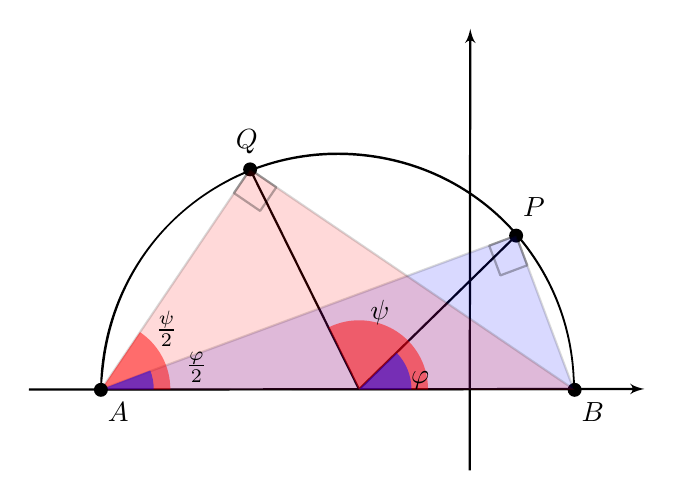
\begin{tikzpicture}[y=0.80pt, x=0.8pt,yscale=-1,scale=0.5, inner sep=0pt, outer sep=0pt]
\begin{scope}[shift={(-152.24647,-317.69709)}]% layer1
  \begin{scope}[shift={(3051.4825,-2552.5587)}]% g2090
    % path2136
    \path[draw=black,line join=miter,line cap=butt,line width=0.800pt,-latex']
      (-2899.2355,3196.2122) -- (-2343.0818,3195.6182);

    % path2138
    \path[draw=black,line join=miter,line cap=butt,line width=0.800pt,-latex']
      (-2500.9667,3269.2615) -- (-2500.3969,2870.2565);

    % path2150
    \path[cm={{0.82575,0.0,0.0,-0.82575,(-129.59075,4772.4814)}},color=black,fill=black,line
      width=0.800pt] (-3275.1575,1929.8205) .. controls (-3272.6894,1957.3643) and
      (-3265.9839,1984.5141) .. (-3255.1425,2009.9408) .. controls
      (-3242.0491,2040.6458) and (-3222.9907,2068.8007) .. (-3199.3033,2092.3240) ..
      controls (-3199.3033,2092.3240) and (-3199.3033,2092.3240) ..
      (-3199.3033,2092.3241) .. controls (-3196.4103,2095.1970) and
      (-3193.4485,2098.0006) .. (-3190.4217,2100.7317) .. controls
      (-3168.6890,2120.3413) and (-3143.7349,2136.3849) .. (-3116.7790,2147.8299) ..
      controls (-3084.9683,2161.3350) and (-3050.3963,2168.3422) ..
      (-3015.8189,2168.2784) .. controls (-3015.8189,2168.2784) and
      (-3015.8189,2168.2784) .. (-3015.8188,2168.2784) .. controls
      (-3014.5354,2168.2784) and (-3013.2520,2168.2644) .. (-3011.9688,2168.2424) ..
      controls (-2978.6867,2167.6762) and (-2945.4841,2160.9886) ..
      (-2914.7105,2148.1805) .. controls (-2885.2450,2135.9154) and
      (-2858.0563,2118.0897) .. (-2835.1556,2095.8335) .. controls
      (-2834.0856,2094.7935) and (-2833.0245,2093.7443) .. (-2831.9727,2092.6861) ..
      controls (-2831.9727,2092.6861) and (-2831.9727,2092.6860) ..
      (-2831.9727,2092.6860) .. controls (-2808.3976,2068.9665) and
      (-2789.4599,2040.6911) .. (-2776.6010,2009.8963) .. controls
      (-2764.9339,1981.9527) and (-2758.3364,1951.9686) .. (-2757.0287,1921.8072) ..
      controls (-2756.5734,1917.3341) and (-2756.5896,1914.0291) ..
      (-2756.7880,1911.8819) .. controls (-2756.9863,1909.7347) and
      (-2757.3672,1908.7418) .. (-2757.7360,1908.8475) .. controls
      (-2758.1048,1908.9533) and (-2758.4624,1910.1551) .. (-2758.6982,1912.3990) ..
      controls (-2758.9339,1914.6428) and (-2759.0483,1917.9268) ..
      (-2759.0029,1922.2309) .. controls (-2760.4135,1951.9864) and
      (-2767.0131,1981.5406) .. (-2778.5723,2009.0625) .. controls
      (-2791.3857,2039.5731) and (-2810.2242,2067.5697) .. (-2833.6318,2091.0269) ..
      controls (-2833.6318,2091.0269) and (-2833.6318,2091.0269) ..
      (-2833.6318,2091.0269) .. controls (-2834.3822,2091.7789) and
      (-2835.1372,2092.5262) .. (-2835.8969,2093.2687) .. controls
      (-2858.8246,2115.6803) and (-2886.1286,2133.5847) .. (-2915.7055,2145.8282) ..
      controls (-2945.2555,2158.0619) and (-2977.0525,2164.6041) ..
      (-3008.9626,2165.4804) .. controls (-3011.2401,2165.5434) and
      (-3013.5259,2165.5764) .. (-3015.8188,2165.5794) .. controls
      (-3032.4616,2165.6014) and (-3049.4865,2164.0242) .. (-3066.3551,2160.7364) ..
      controls (-3083.2236,2157.4486) and (-3099.9303,2152.4501) ..
      (-3115.9176,2145.7939) .. controls (-3129.7045,2140.0545) and
      (-3142.9519,2133.0999) .. (-3155.3778,2125.1595) .. controls
      (-3167.8037,2117.2190) and (-3179.4060,2108.2943) .. (-3189.9701,2098.6776) ..
      controls (-3192.7197,2096.1746) and (-3195.3971,2093.6224) ..
      (-3198.0028,2091.0242) .. controls (-3198.0028,2091.0242) and
      (-3198.0028,2091.0242) .. (-3198.0028,2091.0242) .. controls
      (-3210.0648,2078.9970) and (-3220.5978,2065.9980) .. (-3229.7148,2052.2709) ..
      controls (-3238.8319,2038.5438) and (-3246.5375,2024.0841) ..
      (-3252.8469,2008.9704) .. controls (-3257.5845,1997.6231) and
      (-3261.5238,1985.9048) .. (-3264.6712,1973.8324) .. controls
      (-3267.8187,1961.7600) and (-3270.1751,1949.3321) .. (-3271.6857,1936.5521) ..
      controls (-3271.9629,1934.3114) and (-3272.2907,1931.6065) ..
      (-3272.6070,1928.7698) .. controls (-3272.9233,1925.9331) and
      (-3273.2274,1922.9646) .. (-3273.4985,1920.2021) .. controls
      (-3274.0407,1914.6772) and (-3274.4432,1909.9732) .. (-3274.9023,1908.8402) ..
      controls (-3275.0375,1908.5067) and (-3275.1781,1908.4830) ..
      (-3275.3233,1908.8402) .. controls (-3275.3233,1908.8402) and
      (-3275.3233,1908.8402) .. (-3275.3233,1908.8402) .. controls
      (-3275.4627,1909.1829) and (-3275.6065,1909.8763) .. (-3275.7445,1910.9839) ..
      controls (-3275.8931,1913.7528) and (-3275.8877,1916.9070) ..
      (-3275.7695,1920.1457) .. controls (-3275.6510,1923.3838) and
      (-3275.4194,1926.7064) .. (-3275.1575,1929.8205) -- cycle;

    \begin{scope}[shift={(128.03018,71.58882)}]% g2179
      % path2146
      \path[shift={(-1295.4547,1536.4384)},fill=black,nonzero rule]
        (-1285.2569,1449.0822) .. controls (-1285.2569,1452.5629) and
        (-1288.0786,1455.3846) .. (-1291.5593,1455.3846) .. controls
        (-1295.0401,1455.3846) and (-1297.8618,1452.5629) .. (-1297.8618,1449.0822) ..
        controls (-1297.8618,1445.6014) and (-1295.0401,1442.7797) ..
        (-1291.5593,1442.7797) .. controls (-1288.0786,1442.7797) and
        (-1285.2569,1445.6014) .. (-1285.2569,1449.0822) -- cycle;

      % text2154
      \path[fill=black] (-2580.7356,2968.0764) node[above right] (text2154) {$P$};

    \end{scope}
    \begin{scope}[shift={(-129.74541,14.21761)}]% g2179-7
      \begin{scope}% g2215
        % path2146-4
        \path[shift={(-1277.9852,1533.9696)},fill=black,nonzero rule]
          (-1285.2569,1449.0822) .. controls (-1285.2569,1452.5629) and
          (-1288.0786,1455.3846) .. (-1291.5593,1455.3846) .. controls
          (-1295.0401,1455.3846) and (-1297.8618,1452.5629) .. (-1297.8618,1449.0822) ..
          controls (-1297.8618,1445.6014) and (-1295.0401,1442.7797) ..
          (-1291.5593,1442.7797) .. controls (-1288.0786,1442.7797) and
          (-1285.2569,1445.6014) .. (-1285.2569,1449.0822) -- cycle;

        % text2154-2
        \path[fill=black] (-2582.4631,2969.4089) node[above right] (text2154-2) {$Q$};

      \end{scope}
    \end{scope}
    \begin{scope}[shift={(2.0,0)}]% g2238
      % path2146-9
      \path[shift={(-1116.5677,1747.3139)},fill=black,nonzero rule]
        (-1285.2569,1449.0822) .. controls (-1285.2569,1452.5629) and
        (-1288.0786,1455.3846) .. (-1291.5593,1455.3846) .. controls
        (-1295.0401,1455.3846) and (-1297.8618,1452.5629) .. (-1297.8618,1449.0822) ..
        controls (-1297.8618,1445.6014) and (-1295.0401,1442.7797) ..
        (-1291.5593,1442.7797) .. controls (-1288.0786,1442.7797) and
        (-1285.2569,1445.6014) .. (-1285.2569,1449.0822) -- cycle;

      % text2154-1
      \path[fill=black] (-2401.8486,3224.9519) node[above right] (text2154-1) {$B$};

    \end{scope}
    % path1929
    \path[draw=black,line join=miter,line cap=butt,line width=0.800pt]
      (-2600.8619,3195.8935) -- (-2458.9839,3057.1093);

    % path1934
    \path[draw=black,line join=miter,line cap=butt,line width=0.800pt]
      (-2600.8619,3195.8935) -- (-2699.2899,2997.2693);

    % path1938
    \path[draw=black,fill=c0000ff,opacity=0.150,line join=miter,line cap=butt,line
      width=0.800pt] (-2834.2300,3196.1427) -- (-2458.9839,3057.1093) --
      (-2407.1557,3195.6866) -- cycle;

    % path1940
    \path[draw=black,fill=cff0000,opacity=0.150,line join=miter,line cap=butt,line
      width=0.800pt] (-2833.7991,3196.1423) -- (-2699.2899,2997.2693) --
      (-2406.1270,3196.3960) -- cycle;

    % path1946
    \path[shift={(-14.57628,176.42692)},color=black,fill=cff0000,opacity=0.500,nonzero
      rule,line width=4.320pt] (-2613.5947,2963.4748) .. controls
      (-2582.6713,2948.3924) and (-2545.3762,2961.2342) .. (-2530.2939,2992.1575) ..
      controls (-2526.1453,3000.6635) and (-2523.9891,3010.0028) ..
      (-2523.9891,3019.4666) -- (-2586.2856,3019.4666) -- cycle;

    % path1944
    \path[shift={(-14.57628,176.42692)},color=black,fill=c0000ff,opacity=0.500,nonzero
      rule,line width=4.320pt] (-2552.2550,2986.6036) .. controls
      (-2543.7378,2995.4234) and (-2538.9775,3007.2055) .. (-2538.9775,3019.4666) --
      (-2586.2856,3019.4666) -- cycle;

    % path1946-3
    \path[shift={(-247.36972,176.46328)},color=black,fill=cff0000,opacity=0.500,nonzero
      rule,line width=4.320pt] (-2551.4499,2967.8204) .. controls
      (-2534.2807,2979.4011) and (-2523.9891,2998.7569) .. (-2523.9891,3019.4666) --
      (-2586.2856,3019.4666) -- cycle;

    % path1944-0
    \path[shift={(-247.36972,176.46328)},color=black,fill=c0000ff,opacity=0.500,nonzero
      rule,line width=4.320pt] (-2542.1197,3002.5128) .. controls
      (-2540.0426,3007.9239) and (-2538.9775,3013.6705) .. (-2538.9775,3019.4666) --
      (-2586.2856,3019.4666) -- cycle;

    \begin{scope}[shift={(-425.96748,0)}]% g2238-8
      % path2146-9-4
      \path[shift={(-1116.5677,1747.3139)},fill=black,nonzero rule]
        (-1285.2569,1449.0822) .. controls (-1285.2569,1452.5629) and
        (-1288.0786,1455.3846) .. (-1291.5593,1455.3846) .. controls
        (-1295.0401,1455.3846) and (-1297.8618,1452.5629) .. (-1297.8618,1449.0822) ..
        controls (-1297.8618,1445.6014) and (-1295.0401,1442.7797) ..
        (-1291.5593,1442.7797) .. controls (-1288.0786,1442.7797) and
        (-1285.2569,1445.6014) .. (-1285.2569,1449.0822) -- cycle;

      % text2154-1-2
      \path[fill=black] (-2401.8486,3224.9519) node[above right] (text2154-1-2) {$A$};

    \end{scope}
    % rect1984
    \path[cm={{0.82536,0.5646,-0.5646,0.82536,(0.0,0.0)}},color=black,draw=black,opacity=0.300,line
      join=round,line cap=round,miter limit=4.00,dash phase=16.000pt,line
      width=0.800pt,rounded corners=0.0000cm] (-535.6256,3997.8613) rectangle
      (-506.9445,4023.7852);

    % rect1986
    \path[cm={{0.35176,0.93609,-0.93609,0.35176,(0.0,0.0)}},color=black,draw=black,opacity=0.300,line
      join=round,line cap=round,miter limit=4.00,dash phase=16.000pt,line
      width=0.800pt,rounded corners=0.0000cm] (1996.7638,3377.1963) rectangle
      (2025.4449,3403.1202);

    % text1988
    \path[fill=black] (-2553.9409,3195.8933) node[above right] (text1988) {$\varphi$};

    % text1996
    \path[fill=black] (-2590.6707,3137.3328) node[above right] (text1996) {$\psi$};

    % text2004
    \path[fill=black] (-2757.4363,3175.9297) node[above,right] (text2004)
      {$\frac{\varphi}{2}$};

    % text2008
    \path[fill=black] (-2784.7964,3157.2808) node[above right] (text2008)
      {$\frac{\psi}{2}$};

  \end{scope}
\end{scope}

\end{tikzpicture}


\end{center}
Analizując powyższy rysunek łatwo dostrzec, że ten iloraz jest równy
\[d_{\mathcal{H}}(P,Q)=\le|\ln \frac{\operatorname{tg} \frac{\psi}{2}}{\operatorname{tg} \frac{\varphi}{2}}\ri|=\pause\le|\ln \le(\frac{d_{\mathcal{E}}(A,P)}{d_{\mathcal{E}}(B,P)}\le/\frac{d_{\mathcal{E}}(A,Q)}{d_{\mathcal{E}}(B,Q)}\ri.\ri)\ri|\]
gdzie $d_{\mathcal{E}}$ oznacza zwykłą odległość euklidesową.
\end{frame}
%%%%%%next-slide%%%%%
\mode<all>{\midsection{Izometrie płaszczyzny Poincar\'ego}}
Przypomnijmy, że grupa izometrii danej powierzchni $M$ składała się ze 
wszystkich dyfeomorfizmów $f\colon M\to M$ które zachowują pierwszą formę 
podstawową. Podczas dowodu twierdzenia klasyfikacyjnego dla krzywych mieliśmy do 
czynienia z działaniem grupy $E(3)$. Grupa izometrii sfery $S^2$ jest równa 
dokładnie $SO(3)$. 
\begin{frame}{Izometrie płaszczyzny Poincar\'ego}

\mode<article>{Teraz zajmiemy się grupą izometrii płaszczyzny hiperbolicznej.} Rozważmy $\mathcal{H}\subset \mathbb{C}$, \[\mathcal{H}=\{z\in \mathbb{C}\colon \Im(z)>0\}\]jako podzbiór płaszczyzny zespolonej utożsamiając punkt $(u,v)$ z liczbą $u+iv$. 

\pause\begin{definicja}
Niech $a,b,c,d$ będą takimi liczbami rzeczywistymi, że $ad-bc=1$. Zdefiniujmy odpowiadającą im \textbf{specjalną transformację M\"obiusa} jako funkcję 
$T^{a,b}_{c,d}\colon \mathbb{C}\to\mathbb{C}$ zadaną wzorem
\[T^{a,b}_{c,d}(z)\define \frac{az+b}{cz+d}.\]
\end{definicja}

\end{frame}
%%%%%%next-slide%%%%%
\begin{frame}[<+->]

\begin{twierdzenie}
\mode<presentation>{Niech \[T^{a,b}_{c,d}(z)\define \frac{az+b}{cz+d}\] będzie specjalną transformacją M\"obiusa. Wtedy}
\mode<article>{Niech $T^{a,b}_{c,d}(z)$ będzie specjalną transformacją M\"obiusa. Wtedy}
\begin{itemize}
\item $T^{a,b}_{c,d}\colon \mathcal{H}\to\mathcal{H}$ jest bijekcją.
\item składanie specjalnych funkcji M\"oebiusa odpowiada mnożeniu macierzy 
\[T^{A,B}_{C,D}\circ T^{a,b}_{c,d}=
\le[\begin{array}{cc}
     A&B\\
	C&D
     \end{array}
\ri]\cdot
\le[\begin{array}{cc}
     a&b\\
	c&d
     \end{array}
\ri],\] więc specjalne transformacje M\"obiusa tworzą grupę.
\item Każda specjalna transformacja M\"obiusa jest izometrią płaszczyzny Poincar\'ego.
\end{itemize}
\end{twierdzenie}

\end{frame}
%%%%%%next-slide%%%%%
\begin{frame}

\begin{uwaga}
Wszystkie transformacje M\"obiusa tworzą grupę $PGL(2,\R)$. Jest to iloraz grupy liniowej $GL(2,\R)$ przez podgrupę normalną $H=\{I,-I\}$. Specjalne transformacje są jej podgrupą wyznaczoną przez równanie $\det =1$ są oznaczane $PSL(2,\R)$.
\end{uwaga}

\pause Udowodnimy tylko trzecie stwierdzenie, pierwsze dwa jako proste pozostawiamy jako zadania. 

\textcolor{ared}{\textbf{Dowód:}}\\\pause

Niech $z=u+iv$ oraz niech $T(z)=x+iy$. Musimy sprawdzić, że 
\[\mathcal{I}_z=\mathcal{I}_{T(z)}(DT,DT).\]
\pause Musimy więc znaleźć $\frac{\partial T}{\partial u}=T_u$ i $\frac{\partial T}{\partial v}=T_v$ w punkcie $T(z)=x+iy$.

\end{frame}
%%%%%%next-slide%%%%%
\begin{frame}

\begin{multline*}
T(z)=\frac{az+b}{cz+d}=\frac{(az+b)(c\overline{z}+d)}{|cz+d|^2}=\cdots=\\
 =\frac{(ac(u^2+v^2)+u+bd)}{|cz+d|^2}+i\frac{v}{|cz+d|^2}=x+iy.
 \end{multline*}
 Zatem $y=\frac{v}{|cz+d|^2}$. 
\pause\medskip 
 Traktując $T(z)$ jako funkcję jednego argumentu możemy łatwo policzyć jej pochodną:
 \[\frac{dT(z)}{dz}=\frac{a(cz+d)-c(az+d)}{(cz+d)^2}=\frac{1}{(cz+d)^2}.\]

\end{frame}
%%%%%%next-slide%%%%%
\begin{frame}

Z drugiej strony jest to funkcja zespolona, więc spełnia równania Cauchyego-Riemanna:
\begin{align*}
\frac{d T(z)}{d z}&=\frac{\partial \Re T(z)}{\partial u}+i\frac{\partial \Im T(z)}{\partial u}=\frac{\partial x}{\partial u}+i\frac{\partial y}{\partial u}=T_u\\\pause
\frac{d T(z)}{d z}&=-i \frac{\partial \Re T(z)}{\partial v}+\frac{\partial \Im T(z)}{\partial v}=-i\frac{\partial x}{\partial v}+\frac{\partial y}{\partial v}=-iT_v\\
\end{align*}
\pause Policzmy teraz pierwszą formę podstawową na wektorze $T_u$. Mamy 
\begin{multline*}
\mathcal{I}_{T(z)}\le(T_u,T_u\ri)=\frac{1}{y^2}\le[\le(\frac{\partial x}{\partial u}\ri)^2+\le(\frac{\partial y}{\partial u}\ri)^2\ri]=\frac{1}{y^2}|T'(z)|^2=\\\pause
=\frac{1}{y^2}\frac{1}{(cz+d)^4}=\frac{1}{v^2}=g_{11}
\end{multline*}
\end{frame}
%%%%%%next-slide%%%%%
\begin{frame}
Podobnie można sprawdzić, że 
\[\mathcal{I}_{T(z)}\le(T_v,T_v\ri)=\frac{1}{v^2}=g_{22}.\]
\pause Wreszcie z równań Cauchyego-Riemanna wynika, że
\begin{multline*}
\mathcal{I}_{T(z)}\le(T_u,T_v\ri)=
\frac{1}{y^2}\le(\frac{\partial x}{\partial u}\frac{\partial y}{\partial u}+\frac{\partial x}{\partial v}\frac{\partial y}{\partial v}\ri)=\\\pause
=\frac{1}{y^2}\le(\frac{\partial x}{\partial u}\le(-\frac{\partial x}{\partial v}\ri)+\frac{\partial x}{\partial v}\frac{\partial x}{\partial u}\ri)=0=g_{12}
\end{multline*}

\hfill $\square$

\end{frame}
%%%%%%next-slide%%%%%
\begin{frame}

\begin{exercise}
Pokazać, że specjalne transformacje M\"obiusa przenoszą geodezyjne na geodezyjne. 

\pause\footnotesize{\textbf{Podpowiedź:} Pokazać, że następujące macierze generują grupę $PSL(2,\R)$: 
\[\le\{\le(\begin{array}{cc}
     1 & c\\
	0 & 1\\
     \end{array}
\ri),\quad \le(\begin{array}{cc}
     \lambda & 0\\
	0 & \sfrac{1}{\lambda}\\
     \end{array}
\ri),\quad\le(\begin{array}{cc}
     0& -1\\
	1 & 0\\
     \end{array}
\ri)\ri\}.\]
Następnie zinterpretować geometrycznie działanie poszczególnych macierzy.}
\end{exercise}

\end{frame}
%%%%%%next-slide%%%%%
% \mode<article>{Możliwe są oczywiście różnież inne modele geometrii nie-euklidesowych. Jednym z nich jest model Kleina na (otwartym) dysku. Model Poincar\'ego miał tę zaletę, że był konforemny (równokątny), tzn. kąty mierzone na płaszczyźnie Poincar\'ego miały tę samą miarę co kąty euklidesowe. Model Kleina wiernokątny nie jest, ale ma inne zalety, np. proste w tym modelu są faktycznie odcinkami prostych euklidesowych.
% 
% \begin{frame}[<+->]
% \midsection{Model Kleina na dysku }
% 
% Rozważmy sferę jednostkową
% \[S^{2}=\{(x,y,z)\in \R^{3}\colon x^{2}+y^{2}+z^{2}=1\}.\]
% \textbf{Rzutem stereograficznym} z punktu $N=(0,0,1)\in S^{2}$ nazywamy przekształcenie płaszczyzny $\R^2=\{\,(x,y,0)\in \R^{3}\,\}$ w sferę $S^{2}$ przyporządkowujące punktowi $A\in \R^2$ pewien punkt $\in S^{2}$, który jest przecięciem sfery $S^{2}$ i prostej łączącej punkty $(u,v)$ oraz $N$.
% \begin{center}
% $\input{./Marz/fig/FIG9_13.PIC}$
% \end{center}
% \end{frame}
% %%%%%%next-slide%%%%%
% \begin{frame}[<+->]
% Rzut stereograficzny jest bijekcją płaszczyzny $\R^2$ i $S^2\setminus \{N\}$. Na przykład obrazem prostej $l$ prostopadłą do osi $OX$, jest okrąg na sferze przechodzący przez punkt $N$. Okrąg ten jest również przecięciem sfery z płaszczyzną wyznaczoną przez prostą $l$ i punkt $N$. Płaszczyzna tego okręgu jest więc równoległa do osi $OY$. 
% 
% \begin{center}
% $\input{./Marz/fig/FIG9_14.PIC}$
% \end{center}
% 
% \end{frame}
% %%%%%%next-slide%%%%%
% \begin{frame}[<+->]
% 
% Rozważmy teraz złożenie dwóch przekształceń: obcięcia do półpłaszczyzny Poincar\'{e}go ${\mathcal H}\subset {\mathbb{R}}^{2}=\{\,(x,y,0)\in {\mathbb{R}}^{3}\,\}$ rzutu stereograficznego i rzutowania ortogonalnego na płaszczyznę $X-Z$.
% \[W\colon \mathcal{H}\to S^2\setminus{N}\to D^2\subset X-Z.\]
% Funkcja $W$ określa bijekcję półpłaszczyzny Poincar\'{e}go $\mathcal H$ z kołem otwartym \[{\mathcal K}\define\{\,(x,0,z)\in {\mathbb{R}}^{3}\colon x^{2}+z^{2}<1\}.\] Zauważmy, że proste hiperboliczne w $\mathcal H$ przechodzą na cięciwy koła $\mathcal K$.
% 
% Będziemy pomijać $0$ w zapisie punktów z $\mathcal K$.
% 
% \end{frame}
% %%%%%%next-slide%%%%%
% \begin{frame}[<+->]
% 
% \begin{definicja}
% Koło otwarte $\mathcal{K}$ wraz z pierwszą formą podstawową
% \[\mathcal{I}_{\mathcal{K}}=I_{(x,z)}
% =\le[
% \begin{array}{cc}
% \frac{4}{(1-x^2-z^2)^2} & 0\\
% 0 & \frac{4}{(1-x^2-z^2)^2}
% \end{array}
% \ri]
% \]
% nazywamy \textbf{Modelem Kleina} geometrii hiperbolicznej.
% \end{definicja}
% 
% \begin{lemat}
% Odwzorowanie $W\colon \mathcal{H}\to \mathcal{K}$ określone wzorem
% \[W(x+iy)=\frac{x+i(y-1)}{x+i(y+1)}\]jest izometrią.
% Zauważmy, że jest to transformacja M\"obiusa stowarzyszona z macierzą 
% $\le[
% \begin{array}{cc}
% 1 &-1\\
% 1 & 1
% \end{array}
% \ri].$
% \end{lemat}
% \end{frame}}

\mode<all>{\midsection{Torusy o stałej krzywiźnie}}

Widzieliśmy wcześniej, że Twierdzenie Gaussa-Bonneta ujawnia głębokie związki między całkowitą krzywizną powierzchni a jej własnościami topologiczno-kombinatorycznymi (charakterystyka Eulera). W szczególności wynika z niego, że gładkie zanurzenie sfery w przestrzeń euklidesową musi mieć całkowitą krzywiznę dokładnie taką samą jak standardowa (okrągła) sfera (czyli $4\pi$).

\begin{frame}{Torusy o stałej krzywiźnie}
\begin{exercise}
Jak wyglądają geodezyjne na torusie? Wskazać przykład triangulacji (najlepiej geodezyjnej) na torusie. Sprawdzić, że charakterystyka Eulera torusa jest równa $0$.
\end{exercise}
\mode<presentation>{\pause Z twierdzenia Gaussa-Bonneta wynika, że jeśli $M$ jest homeomorficzna z torusem $T^2$ wtedy jej całkowita krzywizna musi być równa $2\pi \chi(T^2)=0$.}
\end{frame}
Zatem (ponownie na podstawie twierdzenia Gaussa-Bonneta) jeśli powierzchnia $M$ jest homeomorficzna z torusem $T^2$, wtedy jej całkowita krzywizna musi być równa $2\pi \chi(T^2)=0$.

Oczywiście nie istnieje gładkie zanurzenie \textit{płaskiego} torusa w $\R^3$ (tj. o stałej krzywiźnie równej $0$) (pokażemy to później). Możemy jednak w łatwy sposób wskazać płaskie zanurzenie $T^2$w przestrzeń $\R^4$! Na początek przypomnijmy, że torus może być utożsamiony z $S^1\times S^1$. Wtedy sposób zanurzenia na $4$ współrzędne jest narzucający się.

\begin{frame}
\mode<presentation>{
Jak przekonamy się za chwilę nie istnieje gładkie zanurzenie \textit{płaskiego} 
torusa w $\R^3$ (tj. o stałej krzywiźnie równej $0$). Możemy jednak w łatwy 
sposób wskazać płaskie zanurzenie $T^2$w przestrzeń $\R^4$. Na początek 
przypomnijmy, że torus może być utożsamiony z $S^1\times S^1$. } \pause Rozważmy 
kwadrat $U=[0,2\pi)\times [0,2\pi)\subset \R^2$. Niech $x\colon U\to \R^4$ 
będzie określone wzorem

\mode<presentation>{\begin{tabular}{m{2.2in} m{2in}}}
\mode<article>{\begin{tabular}{m{3in} m{2in}}}
$x(u,v)= (\cos u, \sin u,\cos v,\sin v)$& $ \text{
\definecolor{cffff00}{RGB}{255,255,0}
\usetikzlibrary{arrows}

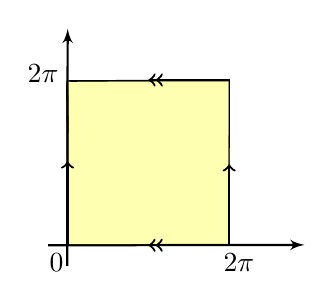
\begin{tikzpicture}[y=0.80pt, x=0.8pt,yscale=-1,scale=0.3, inner sep=0pt, outer sep=0pt]
\begin{scope}[shift={(16.51171,-222.86883)}]% layer1
  \begin{scope}[shift={(920.7302,-2377.8427)}]% g2127
    \begin{scope}[shift={(1217.3295,178.01263)}]% g1961-2
      % path1880-3
      \path[draw=black,line join=miter,line cap=butt,line width=0.800pt,-latex']
        (-2134.6966,2748.6554) -- (-1748.5202,2748.0614);

      % path1882-7
      \path[draw=black,line join=miter,line cap=butt,line width=0.800pt,-latex']
        (-2105.6782,2779.7419) -- (-2105.1084,2422.6997);

    \end{scope}
    % rect1989
    \path[shift={(5.63871,301.66294)},color=black,draw=black,fill=cffff00,opacity=0.300,line
      join=round,line cap=round,miter limit=4.00,nonzero rule,dash
      phase=16.000pt,line width=0.800pt,rounded corners=0.0000cm]
      (-893.5422,2377.1589) rectangle (-650.2519,2624.5854);

    % rect1991
    \path[shift={(5.63871,301.66294)},color=black,fill=black,line width=0.800pt]
      (-895.5773,2402.7889) .. controls (-895.0931,2439.8706) and
      (-894.8552,2476.9218) .. (-894.6665,2513.9962) .. controls
      (-894.4778,2551.0706) and (-894.3383,2588.1683) .. (-894.1753,2625.2185) ..
      controls (-889.8501,2625.2085) and (-885.5248,2625.2025) ..
      (-881.1998,2625.1925) .. controls (-842.5575,2625.1105) and
      (-804.0385,2625.1285) .. (-765.4531,2625.1585) .. controls
      (-726.8677,2625.1885) and (-688.2159,2625.2295) .. (-649.6450,2625.1925) ..
      controls (-649.6470,2623.5864) and (-649.6480,2621.9803) ..
      (-649.6500,2620.3740) .. controls (-649.6720,2600.6502) and
      (-649.6530,2580.9725) .. (-649.6133,2561.2826) .. controls
      (-649.5739,2541.5926) and (-649.5143,2521.8904) .. (-649.4559,2502.1579) ..
      controls (-649.3974,2482.4254) and (-649.3400,2462.6626) ..
      (-649.3049,2442.8918) .. controls (-649.2697,2423.1210) and
      (-649.2569,2403.3422) .. (-649.2874,2383.6180) .. controls
      (-649.2914,2381.1471) and (-649.2954,2378.6765) .. (-649.2990,2376.2062) ..
      controls (-725.6595,2376.0301) and (-801.9274,2375.9960) ..
      (-877.8829,2376.3768) .. controls (-888.7046,2375.7994) and
      (-893.7886,2376.7187) .. (-893.5329,2377.6405) .. controls
      (-893.2773,2378.5623) and (-887.7494,2379.4189) .. (-877.3298,2378.7339) ..
      controls (-801.9695,2378.1316) and (-726.3742,2377.8718) ..
      (-650.7634,2377.6706) .. controls (-650.7624,2379.6122) and
      (-650.7614,2381.5540) .. (-650.7604,2383.4958) .. controls
      (-650.7501,2402.8264) and (-650.7829,2422.2016) .. (-650.8374,2441.5592) ..
      controls (-650.8919,2460.9169) and (-650.9680,2480.2570) ..
      (-651.0445,2499.5579) .. controls (-651.1210,2518.8588) and
      (-651.1979,2538.1204) .. (-651.2537,2557.3611) .. controls
      (-651.3096,2576.6018) and (-651.3444,2595.8216) .. (-651.3370,2615.0791) ..
      controls (-651.3360,2617.8781) and (-651.3340,2620.6870) ..
      (-651.3320,2623.5052) .. controls (-688.6463,2623.5312) and
      (-727.4750,2623.6321) .. (-766.3569,2623.7446) .. controls
      (-805.2388,2623.8572) and (-844.1743,2623.9814) .. (-881.4471,2624.0545) ..
      controls (-885.3264,2624.0645) and (-889.1860,2624.0675) ..
      (-893.0273,2624.0715) .. controls (-892.9843,2587.6801) and
      (-892.7535,2552.6287) .. (-892.5065,2517.6202) .. controls
      (-892.2595,2482.6118) and (-891.9950,2447.6476) .. (-892.2515,2411.0634) ..
      controls (-892.3374,2404.0338) and (-892.6752,2393.2709) ..
      (-893.2271,2385.7558) .. controls (-893.7789,2378.2407) and
      (-894.5527,2373.9655) .. (-895.3643,2380.0575) .. controls
      (-895.7663,2386.7333) and (-895.6353,2395.2566) .. (-895.5773,2402.7889) --
      cycle;

    % text2107
    \path[shift={(5.63871,301.66294)},fill=black] (-920.45374,2665.) node[above
      right] (text2107) {$0$};

    % text2111
    \path[shift={(5.63871,301.66294)},fill=black] (-658.7821,2665.) node[above
      right] (text2111) {$2\pi$};

    % text2115
    \path[shift={(5.63871,301.66294)},fill=black] (-953.63062,2380.092) node[above
      right] (text2115) {$2\pi$};

    % path2119
    \path[shift={(5.63871,301.66294)},draw=black,line join=miter,line cap=butt,line
      width=0.800pt,->>] (-644.1132,2624.9604) -- (-771.8971,2624.9604);

    % path2121
    \path[draw=black,line join=miter,line cap=butt,line width=0.800pt,->]
      (-644.6132,2926.7484) -- (-644.6132,2804.7077);

    % path2123
    \path[draw=black,line join=miter,line cap=butt,line width=0.800pt,->>]
      (-644.1132,2677.8219) -- (-766.1539,2677.8219);

    % path2125
    \path[draw=black,line join=miter,line cap=butt,line width=0.800pt,->]
      (-887.9035,2926.7484) -- (-887.9035,2800.3626);

  \end{scope}
\end{scope}

\end{tikzpicture}

}$
\end{tabular}

\pause Zauważmy, że funkcje $\cos$ i $\sin$ we wzorze powyżej wyrażają utożsamienie przeciwległych brzegów kwadratu.

\end{frame}

\begin{frame}
Niezrażeni faktem, że tym razem $x_1$ i $x_2$ mają po $4$ współrzędne możemy policzyć współczynniki metryczne:
\begin{align*}
g_{11}=&\langle x_1,x_1\rangle=\|x_1\|^2=1\\
g_{12}=&\langle x_1,x_2\rangle=0\\
g_{22}=&\langle x_2,x_2\rangle=\|x_2\|^2=1,\\
\end{align*}
\pause zatem nasz torus zanurzony w $\R^4$ jest faktycznie lokalnie izometryczny z płaszczyzną (więc płaski).

\end{frame}
\mode<all>{\lowsection{Torus genusu $g$}}

\begin{frame}
\mode<article>{\begin{center}}

\definecolor{caa0000}{RGB}{170,0,0}
\definecolor{cffff00}{RGB}{255,255,0}


\mode<presentation>{\begin{tikzpicture}[y=0.80pt, x=0.8pt,yscale=-1,scale=0.23, inner sep=0pt, outer sep=0pt]}
\mode<article>{\begin{tikzpicture}[y=0.80pt, x=0.8pt,yscale=-1,scale=0.3, inner sep=0pt, outer sep=0pt]}
\begin{scope}[shift={(296.85925,-6.26562)}]% layer1
  \begin{scope}[shift={(-138.30846,-2572.6617)}]% g3047
    \begin{scope}% g3001
      % path1960-2
      \path[fill=black] (602.2569,2666.1063) .. controls (608.8543,2667.5163) and
        (615.4214,2669.0941) .. (621.9517,2670.8069) .. controls (645.2314,2676.9148)
        and (668.0892,2684.7134) .. (690.9312,2692.6175) .. controls
        (690.9313,2692.6175) and (690.9313,2692.6175) .. (690.9313,2692.6175) ..
        controls (713.6254,2700.4728) and (736.3448,2708.4558) .. (759.5500,2714.9661)
        .. controls (782.5897,2721.4320) and (806.1639,2726.3984) ..
        (830.0976,2728.2092) .. controls (855.6521,2730.1279) and (881.2661,2726.7043)
        .. (906.2147,2721.4696) .. controls (931.9644,2716.0739) and
        (957.2081,2708.7397) .. (982.6171,2702.3004) .. controls (982.6171,2702.3004)
        and (982.6171,2702.3004) .. (982.6171,2702.3004) .. controls
        (1007.1942,2696.0778) and (1032.0329,2690.5309) .. (1057.2439,2689.1255) ..
        controls (1063.1381,2688.7962) and (1069.0477,2688.7016) ..
        (1074.9423,2688.8943) .. controls (1081.0666,2689.0945) and
        (1087.1746,2689.6068) .. (1093.2317,2690.4899) .. controls
        (1105.1812,2692.2312) and (1116.9265,2695.4409) .. (1128.0153,2700.2043) ..
        controls (1128.0153,2700.2043) and (1128.0153,2700.2043) ..
        (1128.0153,2700.2043) .. controls (1143.4760,2706.8433) and
        (1158.1783,2715.2307) .. (1172.0374,2724.8142) .. controls
        (1172.0374,2724.8142) and (1172.0374,2724.8142) .. (1172.0374,2724.8142) ..
        controls (1186.7210,2734.9712) and (1200.4830,2746.5149) ..
        (1212.4696,2759.7087) .. controls (1223.5702,2771.9378) and
        (1233.2750,2785.6413) .. (1239.0729,2800.9999) .. controls
        (1241.7224,2808.0117) and (1243.5125,2815.3569) .. (1244.0521,2822.7993) ..
        controls (1244.5891,2830.1768) and (1243.8724,2837.6487) ..
        (1241.8692,2844.7594) .. controls (1239.9963,2851.4111) and
        (1236.8995,2857.7197) .. (1232.7600,2863.2465) .. controls
        (1232.7600,2863.2465) and (1232.7600,2863.2465) .. (1232.7600,2863.2465) ..
        controls (1228.6619,2868.7248) and (1223.5662,2873.4461) ..
        (1217.9556,2877.4260) .. controls (1205.5260,2886.2522) and
        (1190.8332,2891.5466) .. (1175.9243,2895.3194) .. controls
        (1175.9243,2895.3194) and (1175.9243,2895.3194) .. (1175.9243,2895.3194) ..
        controls (1159.4845,2899.4685) and (1142.5819,2901.6866) ..
        (1125.6311,2903.1627) .. controls (1109.5282,2904.5634) and
        (1093.3500,2905.2042) .. (1077.1591,2905.8541) .. controls
        (1062.8427,2906.4330) and (1048.5120,2905.1445) .. (1034.3747,2902.5511) ..
        controls (1025.3334,2900.8926) and (1016.3726,2898.6940) ..
        (1007.5485,2896.1030) .. controls (984.3615,2889.2916) and
        (961.9847,2879.8915) .. (939.7300,2870.2675) .. controls (917.2828,2860.5569)
        and (894.9011,2850.5228) .. (871.7505,2842.3671) .. controls
        (871.7504,2842.3671) and (871.7504,2842.3671) .. (871.7504,2842.3671) ..
        controls (849.0906,2834.3801) and (825.5627,2828.2451) .. (801.4729,2826.5876)
        .. controls (785.8192,2825.5192) and (770.0871,2826.6046) ..
        (754.6351,2829.0448) .. controls (754.6350,2829.0448) and (754.6350,2829.0448)
        .. (754.6350,2829.0448) .. controls (738.5423,2831.5849) and
        (722.7243,2835.5566) .. (707.1665,2840.2251) .. controls (707.1665,2840.2251)
        and (707.1665,2840.2251) .. (707.1665,2840.2251) .. controls
        (674.9967,2849.8781) and (643.8829,2862.4626) .. (612.4171,2873.6973) ..
        controls (612.4171,2873.6973) and (612.4170,2873.6973) .. (612.4170,2873.6973)
        .. controls (598.2779,2878.7442) and (584.0632,2883.5393) ..
        (569.6516,2887.5732) .. controls (568.4958,2887.8967) and (567.3388,2888.2152)
        .. (566.1805,2888.5285) .. controls (551.4583,2892.5086) and
        (536.5124,2895.6599) .. (521.3980,2897.1103) .. controls (521.3980,2897.1103)
        and (521.3980,2897.1103) .. (521.3980,2897.1103) .. controls
        (507.1077,2898.4799) and (492.6459,2898.3032) .. (478.5818,2895.7631) ..
        controls (478.5818,2895.7631) and (478.5818,2895.7631) .. (478.5818,2895.7631)
        .. controls (464.3665,2893.2011) and (450.5926,2888.1557) ..
        (438.1227,2880.8625) .. controls (426.2561,2873.9341) and (416.0289,2864.3087)
        .. (407.3975,2853.4898) .. controls (407.3975,2853.4898) and
        (407.3975,2853.4898) .. (407.3975,2853.4898) .. controls (398.2160,2841.9697)
        and (390.8232,2829.0244) .. (385.3759,2815.3148) .. controls
        (385.3759,2815.3148) and (385.3759,2815.3148) .. (385.3759,2815.3148) ..
        controls (380.0178,2801.8162) and (376.5211,2787.5352) .. (375.7611,2773.0713)
        .. controls (375.0585,2759.5800) and (376.7853,2745.8486) ..
        (382.0793,2733.5042) .. controls (382.0793,2733.5042) and (382.0793,2733.5042)
        .. (382.0793,2733.5042) .. controls (388.4771,2718.5301) and
        (398.8150,2705.3592) .. (411.0803,2694.5247) .. controls (424.1156,2683.0148)
        and (439.3218,2674.0255) .. (455.4483,2667.3965) .. controls
        (455.4483,2667.3965) and (455.4483,2667.3965) .. (455.4483,2667.3965) ..
        controls (472.0719,2660.5660) and (489.7303,2656.2247) .. (507.6419,2654.6300)
        .. controls (514.5120,2654.0191) and (521.4284,2653.8136) ..
        (528.3233,2654.0596) .. controls (533.8814,2654.4213) and (538.6697,2654.9488)
        .. (542.7243,2655.4757) .. controls (546.7789,2656.0027) and
        (550.1015,2656.5285) .. (552.7303,2656.9354) .. controls (555.3592,2657.3422)
        and (557.2950,2657.6297) .. (558.5613,2657.7360) .. controls
        (559.8276,2657.8423) and (560.4243,2657.7670) .. (560.3557,2657.5102) ..
        controls (560.2871,2657.2532) and (559.5525,2656.8144) .. (558.1427,2656.2550)
        .. controls (556.7329,2655.6956) and (554.6469,2655.0160) ..
        (551.8749,2654.3346) .. controls (549.1030,2653.6532) and (545.6438,2652.9709)
        .. (541.5055,2652.4514) .. controls (537.3672,2651.9319) and
        (532.5482,2651.5768) .. (527.0954,2651.5764) .. controls (520.5334,2651.3884)
        and (513.9602,2651.6014) .. (507.4315,2652.1771) .. controls
        (489.2675,2653.7753) and (471.3623,2658.1562) .. (454.4983,2665.0647) ..
        controls (454.4983,2665.0647) and (454.4983,2665.0647) .. (454.4983,2665.0647)
        .. controls (438.1360,2671.7636) and (422.6810,2680.8843) ..
        (409.3832,2692.5912) .. controls (396.8576,2703.6132) and (386.2815,2717.0802)
        .. (379.6691,2732.4656) .. controls (379.6691,2732.4656) and
        (379.6690,2732.4656) .. (379.6690,2732.4656) .. controls (374.1869,2745.2666)
        and (372.3737,2759.3902) .. (373.0970,2773.2057) .. controls
        (373.8658,2788.0049) and (377.4085,2802.5741) .. (382.8518,2816.3111) ..
        controls (382.8518,2816.3111) and (382.8518,2816.3111) .. (382.8518,2816.3111)
        .. controls (388.3772,2830.2660) and (395.8899,2843.4513) ..
        (405.2352,2855.2057) .. controls (405.2352,2855.2057) and (405.2352,2855.2057)
        .. (405.2352,2855.2057) .. controls (414.0112,2866.2518) and
        (424.4843,2876.1111) .. (436.7026,2883.2804) .. controls (449.4555,2890.7553)
        and (463.5324,2895.9301) .. (478.0713,2898.5665) .. controls
        (478.0713,2898.5665) and (478.0714,2898.5665) .. (478.0714,2898.5665) ..
        controls (492.4458,2901.1700) and (507.1693,2901.3732) .. (521.6703,2899.9914)
        .. controls (521.6703,2899.9914) and (521.6703,2899.9914) ..
        (521.6703,2899.9914) .. controls (537.0009,2898.5315) and (552.1115,2895.3664)
        .. (566.9440,2891.3681) .. controls (567.1009,2891.3261) and
        (567.2576,2891.2831) .. (567.4144,2891.2410) .. controls (582.9733,2887.0279)
        and (598.2609,2881.9122) .. (613.4235,2876.5171) .. controls
        (613.4236,2876.5171) and (613.4236,2876.5171) .. (613.4236,2876.5171) ..
        controls (644.9840,2865.2893) and (676.0661,2852.7532) .. (708.0639,2843.1939)
        .. controls (708.0639,2843.1939) and (708.0639,2843.1939) ..
        (708.0639,2843.1939) .. controls (723.5385,2838.5711) and (739.2244,2834.6467)
        .. (755.1342,2832.1556) .. controls (770.4081,2829.7651) and
        (785.9048,2828.7060) .. (801.2638,2829.7760) .. controls (824.9549,2831.4132)
        and (848.1918,2837.5112) .. (870.6761,2845.4429) .. controls
        (870.6761,2845.4429) and (870.6761,2845.4429) .. (870.6761,2845.4429) ..
        controls (893.6518,2853.5538) and (915.9530,2863.5764) .. (938.4194,2873.3104)
        .. controls (960.6864,2882.9637) and (983.1832,2892.4227) ..
        (1006.6014,2899.3233) .. controls (1013.0521,2901.2257) and
        (1019.5838,2902.9193) .. (1026.1753,2904.3480) .. controls
        (1042.7934,2907.9499) and (1059.9569,2909.9165) .. (1077.2926,2909.2172) ..
        controls (1093.3774,2908.5604) and (1109.6175,2907.8975) ..
        (1125.9175,2906.4497) .. controls (1142.8803,2904.9458) and
        (1159.9634,2902.6672) .. (1176.7030,2898.3996) .. controls
        (1191.7769,2894.5726) and (1206.8154,2889.0784) .. (1219.7123,2879.9007) ..
        controls (1225.5284,2875.7555) and (1230.8315,2870.7995) ..
        (1235.1342,2865.0214) .. controls (1235.1342,2865.0214) and
        (1235.1342,2865.0214) .. (1235.1342,2865.0214) .. controls
        (1239.4743,2859.1827) and (1242.7070,2852.5419) .. (1244.6525,2845.5407) ..
        controls (1246.7219,2838.0875) and (1247.4437,2830.2856) ..
        (1246.8560,2822.5929) .. controls (1246.2604,2814.8381) and
        (1244.3851,2807.2398) .. (1241.6274,2800.0319) .. controls
        (1235.5761,2784.2363) and (1225.6365,2770.2890) .. (1214.3681,2757.9825) ..
        controls (1202.1316,2744.6038) and (1188.1748,2732.9833) ..
        (1173.4117,2722.8281) .. controls (1159.3332,2713.1401) and
        (1144.4587,2704.7201) .. (1128.9321,2698.0756) .. controls
        (1128.9321,2698.0756) and (1128.9321,2698.0756) .. (1128.9321,2698.0756) ..
        controls (1117.5745,2693.2170) and (1105.6271,2689.9814) ..
        (1093.5649,2688.2297) .. controls (1086.5152,2687.2065) and
        (1079.4353,2686.6777) .. (1072.3792,2686.5452) .. controls
        (1067.2746,2686.4492) and (1062.1824,2686.5592) .. (1057.1203,2686.8403) ..
        controls (1044.2259,2687.5564) and (1031.5441,2689.3175) ..
        (1019.0391,2691.6533) .. controls (1006.5342,2693.9890) and
        (994.2062,2696.9002) .. (982.0257,2699.9540) .. controls (956.3308,2706.3914)
        and (931.1372,2713.6099) .. (905.6668,2718.8400) .. controls
        (880.7558,2723.9494) and (855.4306,2727.2303) .. (830.3270,2725.2222) ..
        controls (806.7216,2723.3473) and (783.4097,2718.3484) .. (760.4362,2711.8288)
        .. controls (737.5499,2705.3320) and (714.9514,2697.3347) ..
        (692.0631,2689.3760) .. controls (669.4851,2681.5231) and (646.5885,2673.6770)
        .. (622.8434,2667.4650) .. controls (621.9366,2667.2277) and
        (621.0284,2666.9929) .. (620.1190,2666.7607) .. controls (613.0231,2664.9693)
        and (603.9707,2662.9349) .. (594.7254,2661.3073) .. controls
        (585.4801,2659.6797) and (576.0468,2658.4807) .. (568.2786,2657.8683) ..
        controls (560.5104,2657.2559) and (554.4148,2657.1954) .. (551.8295,2657.4077)
        .. controls (550.5369,2657.5138) and (550.1208,2657.6840) ..
        (550.8023,2657.9185) .. controls (551.4837,2658.1531) and (553.2628,2658.4487)
        .. (556.3515,2658.8906) .. controls (563.1429,2659.6150) and
        (570.8477,2660.5469) .. (578.7409,2661.7622) .. controls (586.6341,2662.9776)
        and (594.7145,2664.4726) .. (602.2569,2666.1063) -- cycle;

      % path1962-2
      \path[fill=black] (619.3745,2770.9008) .. controls (618.6070,2771.6305) and
        (617.8211,2772.3460) .. (617.0209,2773.0497) .. controls (611.6964,2777.7309)
        and (605.8093,2781.8044) .. (599.6112,2785.3407) .. controls
        (599.6112,2785.3407) and (599.6112,2785.3407) .. (599.6112,2785.3407) ..
        controls (593.0668,2789.0734) and (586.1660,2792.1909) .. (579.0511,2794.7342)
        .. controls (576.6921,2795.5774) and (574.2984,2796.3267) ..
        (571.8788,2796.9832) .. controls (565.9266,2798.5987) and (559.8192,2799.6416)
        .. (553.6756,2800.1873) .. controls (547.5320,2800.7331) and
        (541.3523,2800.7831) .. (535.1977,2800.4188) .. controls (535.1977,2800.4188)
        and (535.1977,2800.4188) .. (535.1977,2800.4188) .. controls
        (534.2485,2800.3628) and (533.2998,2800.2957) .. (532.3519,2800.2182) ..
        controls (526.6060,2799.7482) and (520.9181,2798.6259) .. (515.3833,2797.0287)
        .. controls (509.8485,2795.4315) and (504.4656,2793.3614) ..
        (499.2456,2790.9814) .. controls (495.3991,2789.2280) and (491.6355,2787.3103)
        .. (487.9215,2785.2888) .. controls (482.4766,2782.3251) and
        (477.2354,2778.9602) .. (472.2282,2775.2682) .. controls (472.2282,2775.2682)
        and (472.2282,2775.2682) .. (472.2282,2775.2682) .. controls
        (466.1141,2770.7584) and (460.3379,2765.7750) .. (454.9988,2760.3395) ..
        controls (453.6277,2758.9437) and (452.2870,2757.5205) .. (450.9915,2756.0580)
        .. controls (450.8746,2755.8044) and (450.7524,2755.5791) ..
        (450.6264,2755.3798) .. controls (450.2021,2754.7091) and (449.7361,2754.3355)
        .. (449.2917,2754.1780) -- (449.2917,2754.1780) .. controls
        (449.0626,2754.0970) and (448.8402,2754.0742) .. (448.6338,2754.1000) --
        (448.6338,2754.1000) .. controls (448.5290,2754.1130) and (448.4286,2754.1380)
        .. (448.3339,2754.1750) .. controls (448.3339,2754.1750) and
        (448.3339,2754.1750) .. (448.3339,2754.1750) .. controls (448.2862,2754.1940)
        and (448.2399,2754.2150) .. (448.1954,2754.2390) .. controls
        (448.1954,2754.2390) and (448.1954,2754.2390) .. (448.1954,2754.2390) ..
        controls (448.1023,2754.2900) and (448.0166,2754.3529) .. (447.9404,2754.4273)
        .. controls (447.9038,2754.4633) and (447.8694,2754.5013) ..
        (447.8374,2754.5424) .. controls (447.8374,2754.5424) and (447.8374,2754.5424)
        .. (447.8374,2754.5424) .. controls (447.7737,2754.6234) and
        (447.7198,2754.7153) .. (447.6771,2754.8147) .. controls (447.6771,2754.8147)
        and (447.6771,2754.8147) .. (447.6771,2754.8147) -- (447.6771,2754.8147) ..
        controls (447.5928,2755.0129) and (447.5545,2755.2453) .. (447.5734,2755.4972)
        .. controls (447.5734,2755.4972) and (447.5734,2755.4972) ..
        (447.5734,2755.4972) -- (447.5734,2755.4972) .. controls (447.6107,2755.9947)
        and (447.8778,2756.5777) .. (448.4629,2757.1375) .. controls
        (448.6672,2757.3329) and (448.9105,2757.5260) .. (449.1964,2757.7121) ..
        controls (450.4827,2759.1929) and (451.8087,2760.6309) .. (453.1600,2762.0369)
        .. controls (458.5400,2767.6349) and (464.3692,2772.7797) ..
        (470.5512,2777.4439) .. controls (470.5512,2777.4439) and (470.5512,2777.4440)
        .. (470.5512,2777.4440) .. controls (475.5333,2781.2039) and
        (480.7594,2784.6471) .. (486.2032,2787.7007) .. controls (490.0684,2789.8689)
        and (493.9951,2791.9291) .. (498.0202,2793.8141) .. controls
        (503.2450,2796.2606) and (508.6416,2798.3990) .. (514.1999,2800.0700) ..
        controls (519.7582,2801.7410) and (525.4793,2802.9427) .. (531.2733,2803.5028)
        .. controls (532.4974,2803.6211) and (533.7327,2803.7155) ..
        (534.9771,2803.7852) .. controls (541.1697,2804.1307) and (547.5696,2803.8970)
        .. (553.9040,2803.1141) .. controls (560.2384,2802.3313) and
        (566.5045,2801.0007) .. (572.4797,2799.2590) .. controls (575.0499,2798.5095)
        and (577.5668,2797.6875) .. (580.0191,2796.8112) .. controls
        (587.4195,2794.1667) and (594.3701,2791.3447) .. (601.0311,2787.9025) ..
        controls (607.4271,2784.5984) and (613.5771,2780.7202) .. (619.2061,2775.7416)
        .. controls (619.2061,2775.7416) and (619.2061,2775.7416) ..
        (619.2061,2775.7416) .. controls (619.5908,2775.4013) and (619.9733,2775.0557)
        .. (620.3529,2774.7043) .. controls (621.2908,2773.7881) and
        (622.5402,2772.2735) .. (623.3113,2770.9083) .. controls (623.6598,2770.2911)
        and (623.9128,2769.7055) .. (624.0079,2769.2304) .. controls
        (624.0514,2769.0134) and (624.0616,2768.8198) .. (624.0341,2768.6569) --
        (624.0341,2768.6569) -- (624.0341,2768.6569) -- (624.0341,2768.6569) ..
        controls (624.1192,2768.6739) and (624.2031,2768.7059) .. (624.2627,2768.7319)
        -- (624.2627,2768.7319) -- (624.2627,2768.7319) .. controls
        (624.3559,2768.8049) and (624.4357,2768.8698) .. (624.4930,2768.9166) ..
        controls (624.6082,2769.0146) and (624.6313,2769.0372) .. (624.4803,2768.8906)
        .. controls (624.3983,2768.8336) and (624.2825,2768.7340) ..
        (624.1161,2768.5895) -- (624.1161,2768.5895) -- (624.1161,2768.5895) ..
        controls (623.9794,2768.4872) and (623.7714,2768.3304) .. (623.4620,2768.0934)
        -- (623.4620,2768.0934) -- (623.4620,2768.0934) .. controls
        (623.3085,2768.0664) and (623.1224,2768.0684) .. (622.8962,2768.1044) ..
        controls (622.8922,2768.1050) and (622.8892,2768.1044) .. (622.8855,2768.1044)
        .. controls (622.4259,2768.3318) and (621.9759,2768.6394) ..
        (621.5300,2768.9919) .. controls (620.7880,2769.5793) and (620.0675,2770.2787)
        .. (619.3745,2770.9008) -- cycle;

      % path1982-0
      \path[fill=black] (602.6291,2780.2568) .. controls (597.5912,2777.3115) and
        (592.5183,2774.4205) .. (587.3230,2771.7692) .. controls (582.1277,2769.1179)
        and (576.8073,2766.7072) .. (571.3320,2764.7577) .. controls
        (565.9832,2762.8532) and (560.5995,2761.0993) .. (555.1085,2759.7144) ..
        controls (549.6175,2758.3296) and (544.0167,2757.3147) .. (538.3299,2756.9120)
        .. controls (538.0609,2756.8930) and (537.7919,2756.8760) ..
        (537.5229,2756.8600) .. controls (531.6967,2756.5191) and (525.8846,2756.3590)
        .. (520.0611,2756.6694) .. controls (514.2376,2756.9799) and
        (508.4068,2757.7647) .. (502.7564,2759.2937) .. controls (491.4554,2762.3516)
        and (480.6168,2767.1166) .. (470.7309,2773.1815) .. controls
        (469.0488,2773.4479) and (468.8650,2774.6511) .. (469.3551,2775.4330) ..
        controls (469.8452,2776.2149) and (470.9820,2776.5948) .. (471.9885,2775.2741)
        .. controls (481.7030,2769.5166) and (492.2926,2765.0399) ..
        (503.2530,2762.2035) .. controls (508.7333,2760.7853) and (514.3720,2760.0944)
        .. (519.9823,2759.8549) .. controls (525.5926,2759.6154) and
        (531.1704,2759.8239) .. (536.7414,2760.1841) .. controls (537.1768,2760.2121)
        and (537.6137,2760.2421) .. (538.0521,2760.2751) .. controls
        (543.4511,2760.6590) and (549.0383,2761.3663) .. (554.5676,2762.4774) ..
        controls (560.0970,2763.5885) and (565.5653,2765.1005) .. (570.6791,2766.9453)
        .. controls (576.0007,2768.8651) and (580.8004,2771.4191) ..
        (585.4691,2774.1365) .. controls (590.1378,2776.8539) and (594.6835,2779.7360)
        .. (599.6273,2782.5090) .. controls (600.5517,2782.9825) and
        (602.0783,2783.5454) .. (603.3110,2783.7066) .. controls (604.5436,2783.8677)
        and (605.4910,2783.6206) .. (605.2316,2782.4167) .. controls
        (604.6666,2781.5000) and (603.5724,2780.8576) .. (602.6291,2780.2568) --
        cycle;

      \begin{scope}[cm={{0.8861,0.0,0.0,0.8861,(122.84989,319.1771)}}]% g2969
        % path1962-7-5
        \path[fill=black] (1167.1867,2803.0537) .. controls (1166.2647,2803.9994) and
          (1165.3176,2804.9262) .. (1164.3510,2805.8369) .. controls
          (1158.4474,2811.3980) and (1151.8767,2816.2812) .. (1144.8884,2820.4750) ..
          controls (1144.8884,2820.4750) and (1144.8884,2820.4750) ..
          (1144.8884,2820.4750) .. controls (1137.7437,2824.7609) and
          (1130.1471,2828.3123) .. (1122.2633,2831.0485) .. controls
          (1119.7011,2831.9378) and (1117.0983,2832.7126) .. (1114.4645,2833.3697) ..
          controls (1108.0454,2834.9725) and (1101.4451,2835.8520) ..
          (1094.8325,2836.0682) .. controls (1088.2200,2836.2844) and
          (1081.5955,2835.8393) .. (1075.0673,2834.7970) .. controls
          (1075.0673,2834.7970) and (1075.0673,2834.7970) .. (1075.0673,2834.7970) ..
          controls (1073.1907,2834.4981) and (1071.3234,2834.1455) ..
          (1069.4661,2833.7432) .. controls (1063.7051,2832.4952) and
          (1058.0961,2830.5570) .. (1052.7209,2828.1205) .. controls
          (1047.3457,2825.6840) and (1042.2026,2822.7506) .. (1037.3041,2819.4930) ..
          controls (1032.2912,2816.1589) and (1027.5181,2812.4960) ..
          (1022.8838,2808.6446) .. controls (1018.1994,2804.7516) and
          (1013.7532,2800.5475) .. (1009.5416,2796.1180) .. controls
          (1009.5416,2796.1180) and (1009.5416,2796.1180) .. (1009.5416,2796.1180) ..
          controls (1003.1918,2789.4365) and (997.3619,2782.2455) ..
          (992.0996,2774.6439) .. controls (990.6466,2772.5446) and (989.2379,2770.4165)
          .. (987.8938,2768.2485) .. controls (987.8343,2768.0531) and
          (987.7712,2767.8700) .. (987.7048,2767.6986) .. controls (987.3437,2766.7662)
          and (986.8890,2766.1821) .. (986.4287,2765.8667) -- (986.4287,2765.8667) ..
          controls (986.1907,2765.7036) and (985.9519,2765.6136) .. (985.7252,2765.5862)
          -- (985.7252,2765.5862) .. controls (985.6099,2765.5722) and
          (985.4979,2765.5742) .. (985.3910,2765.5962) .. controls (985.3910,2765.5962)
          and (985.3910,2765.5962) .. (985.3910,2765.5962) .. controls
          (985.3371,2765.6062) and (985.2846,2765.6182) .. (985.2336,2765.6352) ..
          controls (985.2336,2765.6352) and (985.2336,2765.6352) .. (985.2336,2765.6352)
          .. controls (985.1278,2765.6702) and (985.0288,2765.7212) ..
          (984.9391,2765.7879) .. controls (984.8956,2765.8199) and (984.8544,2765.8559)
          .. (984.8156,2765.8959) .. controls (984.8156,2765.8959) and
          (984.8156,2765.8959) .. (984.8156,2765.8959) .. controls (984.7383,2765.9749)
          and (984.6710,2766.0676) .. (984.6156,2766.1727) .. controls
          (984.6156,2766.1727) and (984.6156,2766.1727) .. (984.6156,2766.1727) --
          (984.6156,2766.1727) .. controls (984.5061,2766.3823) and (984.4451,2766.6427)
          .. (984.4483,2766.9400) .. controls (984.4483,2766.9400) and
          (984.4483,2766.9400) .. (984.4483,2766.9400) -- (984.4483,2766.9400) ..
          controls (984.4543,2767.5259) and (984.7154,2768.2643) .. (985.3531,2769.0494)
          .. controls (985.5008,2769.2313) and (985.6688,2769.4159) ..
          (985.8585,2769.6018) .. controls (987.1846,2771.7818) and (988.5704,2773.9184)
          .. (989.9966,2776.0213) .. controls (995.2605,2783.7841) and
          (1001.1082,2791.1435) .. (1007.4971,2797.9965) .. controls
          (1007.4971,2797.9965) and (1007.4971,2797.9965) .. (1007.4971,2797.9965) ..
          controls (1011.6547,2802.4575) and (1016.0549,2806.7059) ..
          (1020.7035,2810.6599) .. controls (1025.4802,2814.7229) and
          (1030.4192,2818.5976) .. (1035.6317,2822.1322) .. controls
          (1040.5177,2825.4456) and (1045.6591,2828.4401) .. (1051.0456,2830.9498) ..
          controls (1056.4321,2833.4595) and (1062.0655,2835.4832) ..
          (1067.8700,2836.8371) .. controls (1070.0475,2837.3449) and
          (1072.2708,2837.7740) .. (1074.5289,2838.1160) .. controls
          (1081.1728,2839.1174) and (1088.0779,2839.3956) .. (1094.9261,2838.9598) ..
          controls (1101.7743,2838.5240) and (1108.5616,2837.3762) ..
          (1115.0184,2835.6553) .. controls (1117.8291,2834.9056) and
          (1120.5768,2834.0542) .. (1123.2497,2833.1247) .. controls
          (1131.4578,2830.2702) and (1139.1011,2826.9889) .. (1146.3577,2822.9876) ..
          controls (1153.5642,2819.0157) and (1160.4158,2814.3315) ..
          (1166.6419,2808.4451) .. controls (1166.6419,2808.4451) and
          (1166.6419,2808.4451) .. (1166.6419,2808.4451) .. controls
          (1167.1530,2807.9620) and (1167.6599,2807.4705) .. (1168.1619,2806.9699) ..
          controls (1169.1615,2805.9246) and (1170.4867,2804.2407) ..
          (1171.3377,2802.7307) .. controls (1171.7427,2802.0119) and
          (1172.0428,2801.3337) .. (1172.1650,2800.7948) .. controls
          (1172.2210,2800.5489) and (1172.2390,2800.3324) .. (1172.2150,2800.1544) --
          (1172.2150,2800.1544) -- (1172.2150,2800.1544) -- (1172.2150,2800.1544) ..
          controls (1172.2030,2800.0694) and (1172.1800,2799.9934) ..
          (1172.1470,2799.9273) -- (1172.1470,2799.9273) -- (1172.1470,2799.9273) ..
          controls (1172.3314,2800.0714) and (1172.4909,2800.1979) ..
          (1172.6054,2800.2894) .. controls (1172.6054,2800.2894) and
          (1172.6054,2800.2894) .. (1172.6054,2800.2894) .. controls
          (1172.7172,2800.3784) and (1172.7862,2800.4346) .. (1172.7926,2800.4398) ..
          controls (1172.7926,2800.4398) and (1172.7926,2800.4398) ..
          (1172.7926,2800.4398) .. controls (1172.7926,2800.4398) and
          (1172.7926,2800.4398) .. (1172.7926,2800.4398) .. controls
          (1172.7926,2800.4398) and (1172.7926,2800.4398) .. (1172.7926,2800.4398) ..
          controls (1172.7926,2800.4398) and (1172.7926,2800.4398) ..
          (1172.7926,2800.4398) .. controls (1172.7926,2800.4398) and
          (1172.7926,2800.4398) .. (1172.7926,2800.4398) .. controls
          (1172.7926,2800.4398) and (1172.7926,2800.4398) .. (1172.7926,2800.4398) ..
          controls (1172.7933,2800.4403) and (1172.7933,2800.4403) ..
          (1172.7926,2800.4398) .. controls (1172.7926,2800.4398) and
          (1172.7926,2800.4398) .. (1172.7926,2800.4398) .. controls
          (1172.7826,2800.4298) and (1172.7166,2800.3788) .. (1172.5641,2800.2528) ..
          controls (1172.4115,2800.1274) and (1172.1757,2799.9330) ..
          (1171.8349,2799.6504) .. controls (1171.8349,2799.6504) and
          (1171.8349,2799.6504) .. (1171.8349,2799.6504) -- (1171.8349,2799.6504) ..
          controls (1171.7679,2799.6254) and (1171.6914,2799.6084) ..
          (1171.6045,2799.6014) -- (1171.6045,2799.6014) .. controls
          (1171.6045,2799.6014) and (1171.6045,2799.6014) .. (1171.6045,2799.6014) ..
          controls (1171.4413,2799.5914) and (1171.2432,2799.6174) ..
          (1171.0026,2799.6824) .. controls (1170.9926,2799.6824) and
          (1170.9896,2799.6924) .. (1170.9826,2799.6944) .. controls
          (1170.4641,2800.0071) and (1169.9539,2800.4114) .. (1169.4478,2800.8629) ..
          controls (1169.4478,2800.8629) and (1169.4478,2800.8629) ..
          (1169.4478,2800.8629) .. controls (1168.6732,2801.5504) and
          (1167.9159,2802.3426) .. (1167.1867,2803.0537) -- cycle;

        % path1984-3
        \path[fill=black] (1149.7967,2813.6155) .. controls (1144.9677,2809.3313) and
          (1140.0721,2805.1259) .. (1134.9604,2801.2012) .. controls
          (1129.8488,2797.2766) and (1124.5174,2793.6319) .. (1118.8733,2790.5177) ..
          controls (1117.8471,2789.9515) and (1116.8163,2789.3937) ..
          (1115.7796,2788.8456) .. controls (1110.5934,2786.1046) and
          (1105.2525,2783.6330) .. (1099.7316,2781.6211) .. controls
          (1094.2107,2779.6091) and (1088.5075,2778.0590) .. (1082.6879,2777.1919) ..
          controls (1081.5405,2777.0209) and (1080.3915,2776.8607) ..
          (1079.2401,2776.7135) .. controls (1073.3916,2775.9693) and
          (1067.4969,2775.5615) .. (1061.5820,2775.6902) .. controls
          (1055.6671,2775.8190) and (1049.7355,2776.4891) .. (1043.9836,2777.8865) ..
          controls (1043.4474,2778.0168) and (1042.9123,2778.1511) ..
          (1042.3784,2778.2893) .. controls (1030.3415,2781.4076) and
          (1018.9300,2786.4170) .. (1008.2983,2792.5720) .. controls
          (1006.4600,2792.8823) and (1006.1786,2794.1174) .. (1006.6537,2794.9087) ..
          controls (1007.1288,2795.7000) and (1008.3377,2796.0624) ..
          (1009.5206,2794.6846) .. controls (1020.0630,2788.7696) and
          (1031.3050,2784.0134) .. (1043.0552,2781.1332) .. controls
          (1043.4980,2781.0247) and (1043.9415,2780.9188) .. (1044.3857,2780.8158) ..
          controls (1050.0437,2779.5039) and (1055.8640,2778.9203) ..
          (1061.6434,2778.8626) .. controls (1067.4227,2778.8046) and
          (1073.1573,2779.2682) .. (1078.8265,2780.0361) .. controls
          (1079.7402,2780.1589) and (1080.6525,2780.2897) .. (1081.5639,2780.4272) ..
          controls (1087.0847,2781.2598) and (1092.7910,2782.5230) ..
          (1098.4087,2784.2726) .. controls (1104.0264,2786.0221) and
          (1109.5503,2788.2561) .. (1114.6725,2790.8664) .. controls
          (1115.7671,2791.4241) and (1116.8437,2791.9975) .. (1117.9000,2792.5847) ..
          controls (1123.3747,2795.6281) and (1128.1276,2799.2947) ..
          (1132.6736,2803.1542) .. controls (1137.2197,2807.0136) and
          (1141.5675,2811.0731) .. (1146.3286,2815.1605) .. controls
          (1147.2255,2815.8788) and (1148.7376,2816.8430) .. (1150.0007,2817.3215) ..
          controls (1151.2637,2817.7999) and (1152.2882,2817.7865) ..
          (1152.1951,2816.4861) .. controls (1151.7408,2815.4026) and
          (1150.6935,2814.4681) .. (1149.7967,2813.6155) -- cycle;

      \end{scope}
      % path59-5-9
      \path[fill=caa0000] (819.2931,2827.4105) .. controls (817.1515,2826.3185) and
        (815.2409,2824.3951) .. (813.6708,2822.2453) .. controls (811.0864,2818.6390)
        and (809.4179,2814.3350) .. (808.0433,2809.9308) .. controls
        (808.0433,2809.9308) and (808.0433,2809.9308) .. (808.0433,2809.9308) ..
        controls (807.5534,2808.3525) and (807.1026,2806.7609) .. (806.6799,2805.1587)
        .. controls (805.6102,2801.1037) and (804.9935,2796.9267) ..
        (804.6455,2792.7282) .. controls (804.2976,2788.5298) and (804.2167,2784.3077)
        .. (804.2075,2780.0917) .. controls (804.2065,2779.3913) and
        (804.2076,2778.6908) .. (804.2105,2777.9900) .. controls (804.2297,2773.4770)
        and (804.8069,2768.9761) .. (805.5618,2764.5233) .. controls
        (806.3361,2759.9666) and (807.2893,2755.4772) .. (808.2111,2751.0041) ..
        controls (808.4323,2749.9302) and (808.6707,2748.8606) .. (808.9280,2747.7956)
        .. controls (808.9280,2747.7956) and (808.9280,2747.7956) ..
        (808.9280,2747.7956) .. controls (810.1009,2743.0192) and (811.4970,2738.3359)
        .. (814.0220,2734.2953) .. controls (814.0220,2734.2953) and
        (814.0220,2734.2953) .. (814.0220,2734.2953) .. controls (815.0086,2732.7220)
        and (816.1432,2731.2619) .. (817.5657,2730.1715) .. controls
        (817.5657,2730.1715) and (817.5657,2730.1715) .. (817.5657,2730.1715) ..
        controls (818.3765,2729.5461) and (819.2954,2729.0408) .. (820.2752,2728.7160)
        .. controls (820.9076,2728.8488) and (821.2710,2728.7152) ..
        (821.5207,2728.4116) .. controls (821.7703,2728.1081) and (821.8952,2727.6391)
        .. (821.8592,2727.1793) .. controls (821.8232,2726.7194) and
        (821.6105,2726.2692) .. (821.2040,2726.0560) .. controls (820.7974,2725.8428)
        and (820.1864,2725.8735) .. (819.5777,2726.3835) .. controls
        (818.3323,2726.7625) and (817.1748,2727.3548) .. (816.1520,2728.1072) ..
        controls (816.1520,2728.1072) and (816.1520,2728.1072) .. (816.1520,2728.1072)
        .. controls (814.3752,2729.4236) and (812.9900,2731.0804) ..
        (811.8718,2732.8163) .. controls (811.8718,2732.8163) and (811.8717,2732.8163)
        .. (811.8717,2732.8163) .. controls (809.0292,2737.2135) and
        (807.4084,2742.1520) .. (806.1454,2747.0363) .. controls (806.1454,2747.0363)
        and (806.1454,2747.0363) .. (806.1454,2747.0363) .. controls
        (805.8749,2748.0732) and (805.6220,2749.1136) .. (805.3852,2750.1570) ..
        controls (804.3300,2754.8053) and (803.2512,2759.4542) .. (802.3835,2764.1505)
        .. controls (801.5709,2768.5383) and (800.9406,2772.9885) ..
        (800.8490,2777.4681) .. controls (800.8315,2778.3272) and (800.8278,2779.1943)
        .. (800.8379,2780.0675) .. controls (800.8845,2784.3383) and
        (801.2521,2788.7634) .. (801.8899,2793.1195) .. controls (802.5277,2797.4757)
        and (803.4365,2801.7593) .. (804.4929,2805.8047) .. controls
        (804.9156,2807.4234) and (805.3191,2809.0149) .. (805.7295,2810.5894) ..
        controls (806.3344,2812.9218) and (806.9673,2815.2347) .. (807.7798,2817.4968)
        .. controls (808.5923,2819.7588) and (809.5856,2821.9740) ..
        (810.9078,2824.0627) .. controls (812.2845,2826.2728) and (814.1601,2828.3553)
        .. (816.5377,2829.7781) .. controls (816.9353,2829.9934) and
        (817.4784,2830.2051) .. (818.0573,2830.3335) .. controls (818.6362,2830.4618)
        and (819.2490,2830.5050) .. (819.7744,2830.4295) .. controls
        (820.2997,2830.3545) and (820.7344,2830.1617) .. (820.9864,2829.8657) ..
        controls (821.2384,2829.5697) and (821.3058,2829.1761) .. (821.1687,2828.6817)
        .. controls (820.6944,2828.0555) and (819.9377,2827.7864) ..
        (819.2931,2827.4105) -- cycle;

      % path61-2-9
      \path[fill=caa0000,opacity=0.280] (826.7869,2831.0169) .. controls
        (829.4011,2829.1306) and (831.4176,2826.6755) .. (832.9601,2824.0932) ..
        controls (835.5225,2819.8747) and (837.2024,2815.2898) .. (838.3949,2810.6756)
        .. controls (838.3949,2810.6756) and (838.3949,2810.6756) ..
        (838.3949,2810.6756) .. controls (838.8241,2809.0251) and (839.1978,2807.3629)
        .. (839.5106,2805.6908) .. controls (840.3024,2801.4592) and
        (840.9770,2797.2188) .. (841.4394,2792.9447) .. controls (841.9019,2788.6706)
        and (842.1505,2784.3649) .. (842.0803,2780.0739) .. controls
        (842.0689,2779.3600) and (842.0482,2778.6464) .. (842.0179,2777.9333) ..
        controls (841.8225,2773.3411) and (841.7123,2768.7477) .. (841.4061,2764.1543)
        .. controls (841.0946,2759.4536) and (840.5701,2754.7195) ..
        (839.3656,2750.1237) .. controls (839.0764,2749.0204) and (838.7670,2747.9218)
        .. (838.4355,2746.8291) .. controls (838.4355,2746.8291) and
        (838.4355,2746.8291) .. (838.4355,2746.8291) .. controls (836.9770,2741.9618)
        and (835.0571,2737.0238) .. (831.9218,2732.8356) .. controls
        (831.9218,2732.8356) and (831.9218,2732.8356) .. (831.9218,2732.8356) ..
        controls (830.6888,2731.1819) and (829.1920,2729.6451) .. (827.3844,2728.5235)
        .. controls (827.3844,2728.5235) and (827.3844,2728.5235) ..
        (827.3844,2728.5235) .. controls (826.3270,2727.8695) and (825.1597,2727.3987)
        .. (823.9528,2727.1544) .. controls (823.3569,2726.7019) and
        (822.7926,2726.7224) .. (822.4384,2726.9684) .. controls (822.0842,2727.2144)
        and (821.9263,2727.6800) .. (821.9203,2728.1412) .. controls
        (821.9143,2728.6024) and (822.0446,2729.0597) .. (822.2746,2729.3394) ..
        controls (822.5047,2729.6190) and (822.8261,2729.7171) .. (823.3990,2729.5249)
        .. controls (824.2880,2729.7200) and (825.1663,2730.0889) ..
        (825.9707,2730.5878) .. controls (825.9707,2730.5878) and (825.9707,2730.5878)
        .. (825.9707,2730.5878) .. controls (827.4240,2731.4835) and
        (828.6702,2732.8235) .. (829.7716,2734.3146) .. controls (829.7716,2734.3146)
        and (829.7716,2734.3146) .. (829.7716,2734.3146) .. controls
        (832.5894,2738.1463) and (834.2846,2742.8293) .. (835.6529,2747.5884) ..
        controls (835.6529,2747.5884) and (835.6529,2747.5884) .. (835.6529,2747.5884)
        .. controls (835.9400,2748.5948) and (836.2079,2749.6072) ..
        (836.4582,2750.6246) .. controls (837.5732,2755.1573) and (837.9960,2759.8488)
        .. (838.2278,2764.5271) .. controls (838.4426,2768.8980) and
        (838.4892,2773.2509) .. (838.6344,2777.5847) .. controls (838.6623,2778.4158)
        and (838.6882,2779.2540) .. (838.7106,2780.0981) .. controls
        (838.8176,2784.2385) and (838.8569,2788.5318) .. (838.6597,2792.8029) ..
        controls (838.4626,2797.0740) and (838.0255,2801.3226) .. (837.2579,2805.3360)
        .. controls (836.9508,2806.9419) and (836.5506,2808.4997) ..
        (836.0809,2810.0169) .. controls (835.3831,2812.2613) and (834.5348,2814.4152)
        .. (833.5527,2816.4595) .. controls (832.5705,2818.5038) and
        (831.4581,2820.4370) .. (830.1970,2822.2758) .. controls (828.8724,2824.1725)
        and (827.4080,2825.9979) .. (825.6716,2827.5446) .. controls
        (825.1304,2828.0787) and (824.3486,2828.9871) .. (823.7905,2829.8467) ..
        controls (823.5114,2830.2765) and (823.2960,2830.7040) .. (823.2723,2831.0978)
        .. controls (823.2487,2831.4916) and (823.4206,2831.8582) ..
        (823.9481,2832.1008) .. controls (824.9312,2832.1748) and (825.9503,2831.5687)
        .. (826.7869,2831.0169) -- cycle;

      \begin{scope}[shift={(140.0,-40.0)}]% g2996
        % path2892
        \path[shift={(125.63871,501.66294)},color=black,fill=cffff00,opacity=0.300,nonzero
          rule,line width=0.800pt] (-8.9298,2416.9253) -- (-130.3773,2537.6399) --
          (-301.6117,2537.1218) -- (-422.3263,2415.6743) -- (-421.8081,2244.4399) --
          (-300.3607,2123.7253) -- (-129.1262,2124.2435) -- (-8.4116,2245.6909) --
          cycle;

        % path2894
        \path[shift={(125.63871,501.66294)},color=black,draw=black,fill=black,line
          width=0.800pt] (-6.7412,2381.1540) .. controls (-6.9771,2335.7961) and
          (-7.0406,2290.4752) .. (-7.0511,2245.1322) .. controls (-47.6384,2204.4526)
          and (-88.1482,2163.7498) .. (-128.6726,2123.1578) .. controls
          (-128.6726,2123.1578) and (-128.6726,2123.1577) .. (-128.6726,2123.1577) ..
          controls (-135.6726,2123.1477) and (-142.6721,2123.1477) ..
          (-149.6706,2123.1447) .. controls (-200.0669,2123.1237) and
          (-250.3703,2122.9526) .. (-300.7589,2122.7558) .. controls
          (-341.4431,2163.1234) and (-382.2177,2203.5341) .. (-422.8428,2244.0079) ..
          controls (-422.8428,2244.0079) and (-422.8428,2244.0079) ..
          (-422.8428,2244.0079) .. controls (-422.8468,2246.2489) and
          (-422.8508,2248.4899) .. (-422.8547,2250.7309) .. controls
          (-422.9004,2278.3059) and (-423.0169,2305.8445) .. (-423.1680,2333.4152) ..
          controls (-423.3190,2360.9858) and (-423.5045,2388.5886) ..
          (-423.6882,2416.2339) .. controls (-404.4082,2435.7722) and
          (-385.0960,2455.3401) .. (-365.7382,2474.9002) .. controls
          (-346.3803,2494.4603) and (-326.9767,2514.0126) .. (-307.5542,2533.4791) ..
          controls (-305.8003,2535.2371) and (-304.0465,2536.9948) ..
          (-302.2928,2538.7524) .. controls (-302.2928,2538.7524) and
          (-302.2928,2538.7524) .. (-302.2928,2538.7524) .. controls
          (-244.6978,2538.8154) and (-187.1980,2538.8572) .. (-129.8753,2538.8626) ..
          controls (-94.4484,2503.5284) and (-59.0993,2468.2029) .. (-23.8729,2432.8968)
          .. controls (-18.3127,2427.7774) and (-14.4265,2423.7973) ..
          (-12.0559,2421.0518) .. controls (-9.6852,2418.3064) and (-8.8269,2416.7944)
          .. (-9.2784,2416.5932) .. controls (-9.7299,2416.3921) and
          (-11.4882,2417.5006) .. (-14.3534,2419.9973) .. controls (-17.2185,2422.4939)
          and (-21.1876,2426.3776) .. (-26.1055,2431.7450) .. controls
          (-60.9238,2466.6846) and (-95.8419,2501.6330) .. (-130.8127,2536.5801) ..
          controls (-187.5383,2536.5011) and (-244.3769,2536.3859) ..
          (-301.2482,2536.2520) .. controls (-301.2482,2536.2520) and
          (-301.2482,2536.2520) .. (-301.2482,2536.2520) .. controls
          (-302.4847,2535.0096) and (-303.7212,2533.7672) .. (-304.9578,2532.5248) ..
          controls (-324.3793,2513.0107) and (-343.7711,2493.4180) ..
          (-363.1059,2473.8291) .. controls (-382.4407,2454.2402) and
          (-401.7185,2434.6551) .. (-420.9559,2415.1118) .. controls
          (-420.7480,2388.6709) and (-420.5410,2362.2840) .. (-420.3693,2335.9391) ..
          controls (-420.1975,2309.5942) and (-420.0610,2283.2913) ..
          (-419.9939,2256.9655) .. controls (-419.9839,2253.0602) and
          (-419.9747,2249.1413) .. (-419.9662,2245.2097) .. controls
          (-380.9683,2206.3809) and (-340.3543,2165.7450) .. (-299.7838,2125.1303) ..
          controls (-248.6483,2125.1023) and (-197.5651,2125.0613) ..
          (-148.5188,2125.0913) .. controls (-142.1413,2125.0913) and
          (-135.8000,2125.1043) .. (-129.4917,2125.1183) .. controls
          (-129.4916,2125.1183) and (-129.4916,2125.1183) .. (-129.4916,2125.1183) ..
          controls (-108.8773,2145.8209) and (-88.7824,2166.1379) ..
          (-68.9287,2186.2496) .. controls (-49.0750,2206.3613) and (-29.4621,2226.2682)
          .. (-9.7303,2246.2326) .. controls (-10.0203,2286.6935) and
          (-10.2442,2327.3686) .. (-10.1161,2369.6016) .. controls (-10.0486,2379.4136)
          and (-9.7368,2394.4360) .. (-9.2107,2404.9266) .. controls (-8.6846,2415.4172)
          and (-7.9394,2421.3872) .. (-7.0909,2412.8858) .. controls (-6.6499,2403.5670)
          and (-6.7278,2391.6686) .. (-6.7412,2381.1540) -- cycle;

        % path2932
        \path[shift={(5.63871,301.66294)},fill=caa0000] (-12.8123,2726.0621) .. controls
          (-27.0188,2693.3717) and (-40.4585,2660.3094) .. (-54.3393,2627.3931) ..
          controls (-68.2199,2594.4772) and (-81.3380,2561.2149) .. (-95.0850,2528.2050)
          .. controls (-108.8319,2495.1951) and (-121.3576,2461.6776) ..
          (-135.1626,2428.7059) .. controls (-148.9678,2395.7337) and
          (-162.8501,2362.8136) .. (-176.9053,2330.0115) .. controls
          (-179.5847,2320.4438) and (-183.9084,2322.9163) .. (-179.0504,2331.2047) ..
          controls (-165.2762,2363.7698) and (-151.6800,2396.4560) ..
          (-138.1498,2429.1862) .. controls (-124.6197,2461.9164) and
          (-112.3577,2495.1838) .. (-98.8477,2527.9238) .. controls (-85.3375,2560.6636)
          and (-69.9389,2596.1997) .. (-56.2255,2628.7942) .. controls
          (-42.5121,2661.3887) and (-31.6880,2691.5336) .. (-17.5476,2723.8273) ..
          controls (-14.8930,2729.6942) and (-8.6331,2741.4787) .. (-9.1817,2735.7259)
          .. controls (-9.9367,2732.7586) and (-11.4883,2729.2155) ..
          (-12.8123,2726.0621) -- cycle;

      \end{scope}
    \end{scope}
    % text3015
    \path[shift={(5.63871,301.66294)},fill=black] (45.256557,2265.9844) node[above
      right] (text3015) {$a$};

    % text3019
    \path[shift={(5.63871,301.66294)},fill=black] (191.23106,2334.9673) node[above
      right] (text3019) {$b$};

    % text3023
    \path[shift={(5.63871,301.66294)},fill=black] (261.32928,2491.3081) node[above
      right] (text3023) {$a^{-1}$};

    % text3027
    \path[shift={(5.63871,301.66294)},fill=black] (195.34647,2675.2827) node[above
      right] (text3027) {$b^{-1}$};

    % text3031
    \path[shift={(5.63871,301.66294)},fill=black] (44.005531,2732.3809) node[above
      right] (text3031) {$c$};

    % text3035
    \path[shift={(5.63871,301.66294)},fill=black] (-140.96898,2675.3979) node[above
      right] (text3035) {$d$};

    % text3039
    \path[shift={(5.63871,301.66294)},fill=black] (-247.06718,2490.0571) node[above
      right] (text3039) {$c^{-1}$};

    % text3043
    \path[shift={(5.63871,301.66294)},fill=black] (-160.08438,2334.9673) node[above
      right] (text3043) {$d^{-1}$};

  \end{scope}
\end{scope}

\end{tikzpicture}


\mode<article>{\end{center}}
Jeśli utożsamimy opisane krawędzie $8$-kąta zgodnie z przypisaną im orientacją, wtedy otrzymamy podwójny torus po prawej stronie. 
\pause Można pokazać (sprawdzić!), że charakterystyka Eulera podwójnego torusa wynosi $-2$ (ogólniej: dla torusa genusu $g$ to $2-2g$).
\end{frame}

\begin{frame}
Na mocy twierdzenia Gaussa-Bonneta taki torus będzie miał krzywiznę całkowitą równą $-4\pi g$ więc możemy zapytać o zanurzenie o \textit{stałej} krzywiźnie ujemnej, równej $-1$. \pause Wystarczy znaleźć \textbf{foremny} $4g$-kąt foremny zanurzony na płaszczyźnie hiperbolicznej o \textbf{sumie kątów wewnętrznych równej $2\pi$}. Wtedy utożsamienie odpowiednich boków da nam $2$-torus o krzywiźnie indukowanej z $\mathcal{H}$ ($=-1$).

\pause \begin{uwaga}
Nakładamy warunek na sumę kątów wewnętrznych ($=2\pi$) żeby po odpowiednim utożsamieniu brzegów otrzymać \textit{gładką} powierzchnię. Jeśli coś podobnego spóbujemy zrobić na płaszczyźnie Euklidesowej otrzymana powierzchnia nie będzie gładka! (co dzieje się wokół wierzchołka??) 
\end{uwaga}
\end{frame}
\begin{frame}

\begin{center}

\definecolor{c999999}{RGB}{123,123,123}


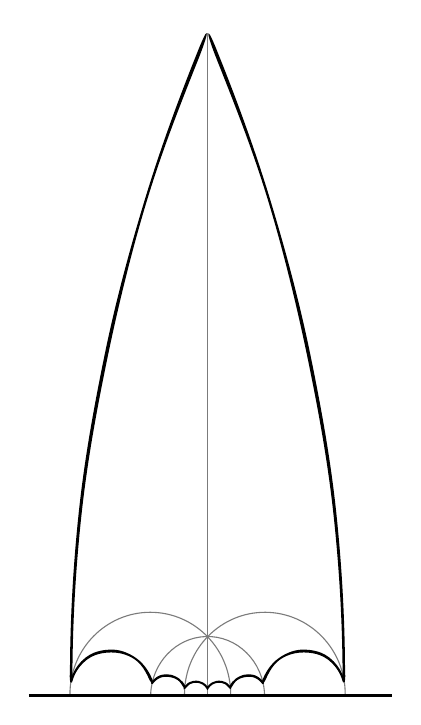
\begin{tikzpicture}[y=0.80pt, x=0.8pt,yscale=-1,scale=0.6, inner sep=0pt, outer sep=0pt]
\begin{scope}[shift={(-247.83596,-128.80023)}]% layer1
  \begin{scope}[draw=c999999]% g3500
    % path2595
    \path[cm={{0.23402,0.0,0.0,-0.23856,(1131.3114,1082.0084)}},color=black,draw=c999999,miter limit=4.00,line width=0.400pt] (-2757.3581,1906.9052) .. controls (-2756.2898,2049.6491) and (-2871.1405,2166.2320) .. (-3013.8844,2167.3003) .. controls (-3156.6284,2168.3687) and (-3273.2113,2053.5179) .. (-3274.2796,1910.7740) .. controls (-3274.2906,1909.3670) and (-3274.2896,1907.9599) .. (-3274.2796,1906.5529);

    % path2629
    \path[cm={{0.16599,0.0,0.0,-0.17548,(882.96488,963.55496)}},color=black,draw=c999999,miter limit=4.00,line width=.4pt] (-2757.4891,1917.2920) .. controls (-2762.1572,2059.9636) and (-2881.5997,2171.8375) .. (-3024.2713,2167.1693) .. controls (-3160.1204,2162.7244) and (-3269.3158,2053.8214) .. (-3274.1250,1917.9847);

    % path2633
    \path[cm={{0.23402,0.0,0.0,-0.23856,(1045.0686,1082.0084)}},color=black,draw=c999999,miter limit=4.00,line width=.40pt] (-2757.3509,1908.8396) .. controls (-2757.3509,2051.5875) and (-2873.0709,2167.3076) .. (-3015.8188,2167.3076) .. controls (-3158.5668,2167.3076) and (-3274.2868,2051.5875) .. (-3274.2868,1908.8396) .. controls (-3274.2868,1908.7536) and (-3274.2868,1908.6674) .. (-3274.2867,1908.5814);

    % path3496
    \path[draw=c999999,line join=miter,line cap=butt,miter limit=4.00,line width=0.40pt] (382.6397,627.1219) -- (382.6397,128.8002);

  \end{scope}
  \begin{scope}% g3506
    % path2025
    \path[cm={{-5.05012,0.0,0.0,-4.94347,(-13645.638,10063.322)}},color=black,fill=black,line width=0.300pt] (-2776.4562,2007.2144) .. controls (-2773.4784,1999.6813) and (-2770.7356,1992.0437) .. (-2768.4210,1984.2665) .. controls (-2766.1064,1976.4892) and (-2764.0338,1968.6285) .. (-2762.4320,1960.6654) .. controls (-2760.8302,1952.7024) and (-2759.4047,1944.6915) .. (-2758.5655,1936.6121) .. controls (-2757.7264,1928.5327) and (-2757.2814,1920.4180) .. (-2757.2530,1912.3139) .. controls (-2757.0493,1910.0753) and (-2757.7916,1910.2146) .. (-2757.6195,1912.3739) .. controls (-2757.6745,1920.3920) and (-2758.1389,1928.4187) .. (-2758.9879,1936.4082) .. controls (-2759.8369,1944.3977) and (-2761.2625,1952.3171) .. (-2762.8512,1960.1880) .. controls (-2764.4400,1968.0590) and (-2766.4897,1976.6061) .. (-2768.7859,1984.2922) .. controls (-2771.0820,1991.9782) and (-2773.7145,1998.7504) .. (-2776.6141,2006.2008) .. controls (-2777.1326,2007.5656) and (-2778.1205,2010.4210) .. (-2777.4003,2009.3608) .. controls (-2777.0736,2008.7515) and (-2776.7478,2007.9348) .. (-2776.4562,2007.2144) -- cycle;

    % path2016
    \path[cm={{5.05012,0.0,0.0,-4.94347,(14410.388,10063.322)}},color=black,fill=black,line width=0.300pt] (-2776.4434,2007.1833) .. controls (-2773.4688,1999.6551) and (-2770.7286,1992.0227) .. (-2768.4162,1984.2508) .. controls (-2766.1038,1976.4789) and (-2764.0328,1968.6238) .. (-2762.4322,1960.6664) .. controls (-2760.8315,1952.7090) and (-2759.4066,1944.7038) .. (-2758.5675,1936.6303) .. controls (-2757.7284,1928.5567) and (-2757.2830,1920.4477) .. (-2757.2535,1912.3494) .. controls (-2757.0495,1910.1124) and (-2757.7918,1910.2515) .. (-2757.6200,1912.4094) .. controls (-2757.6760,1920.4218) and (-2758.1409,1928.4428) .. (-2758.9898,1936.4265) .. controls (-2759.8388,1944.4103) and (-2761.2638,1952.3240) .. (-2762.8514,1960.1893) .. controls (-2764.4390,1968.0547) and (-2766.4870,1976.5958) .. (-2768.7811,1984.2765) .. controls (-2771.0751,1991.9573) and (-2773.7052,1998.7249) .. (-2776.6016,2006.1704) .. controls (-2777.1196,2007.5343) and (-2778.1062,2010.3878) .. (-2777.3866,2009.3284) .. controls (-2777.0602,2008.7193) and (-2776.7347,2007.9033) .. (-2776.4434,2007.1833) -- cycle;

    % path2597
    \path[cm={{0.12271,0.0,0.0,-0.1288,(825.04927,872.99186)}},color=black,fill=black,line width=1.922pt] (-3270.6566,1995.5481) .. controls (-3263.0115,2013.9487) and (-3253.8808,2031.5560) .. (-3243.1627,2048.0992) .. controls (-3232.4445,2064.6424) and (-3220.1303,2080.1166) .. (-3206.1966,2093.9898) .. controls (-3195.1005,2105.0323) and (-3183.0000,2115.0315) .. (-3170.0513,2123.7229) .. controls (-3157.8195,2131.9332) and (-3145.1069,2139.3623) .. (-3131.9154,2145.8447) .. controls (-3118.7240,2152.3271) and (-3105.0523,2157.8605) .. (-3090.9774,2162.2145) .. controls (-3078.8926,2165.9515) and (-3066.5277,2168.8291) .. (-3054.0052,2170.7288) .. controls (-3041.4827,2172.6286) and (-3028.8024,2173.5492) .. (-3016.1414,2173.3756) .. controls (-3006.2171,2173.2395) and (-2996.3054,2172.7608) .. (-2986.4112,2171.8460) .. controls (-2986.4112,2171.8460) and (-2986.4112,2171.8460) .. (-2986.4112,2171.8460) .. controls (-2969.4628,2170.2759) and (-2952.5774,2167.4393) .. (-2936.0285,2162.9898) .. controls (-2919.4796,2158.5402) and (-2903.2706,2152.4684) .. (-2887.9702,2144.5225) .. controls (-2878.1889,2139.4424) and (-2868.7927,2133.6030) .. (-2859.9701,2127.0070) .. controls (-2841.1783,2112.9578) and (-2824.3263,2096.4325) .. (-2810.0770,2077.9819) .. controls (-2790.6001,2052.7502) and (-2776.1147,2023.9849) .. (-2767.4455,1993.8212) .. controls (-2764.8634,1990.7382) and (-2764.4670,1987.9284) .. (-2765.2768,1985.8068) .. controls (-2766.0865,1983.6852) and (-2768.0976,1982.2376) .. (-2770.3321,1981.6648) .. controls (-2772.5666,1981.0920) and (-2775.0214,1981.3807) .. (-2776.7757,1982.7257) .. controls (-2778.5301,1984.0707) and (-2779.5800,1986.4608) .. (-2779.1119,1990.2694) .. controls (-2787.7742,2018.7575) and (-2801.9199,2045.7888) .. (-2820.6283,2069.3000) .. controls (-2834.1684,2086.3226) and (-2850.0781,2101.5279) .. (-2867.7008,2114.4266) .. controls (-2876.3770,2120.7770) and (-2885.6279,2126.3399) .. (-2895.2412,2131.1189) .. controls (-2909.8059,2138.3598) and (-2925.1949,2143.8002) .. (-2940.8389,2147.7229) .. controls (-2956.4829,2151.6456) and (-2972.3783,2154.0604) .. (-2988.2637,2155.3428) .. controls (-2996.7255,2156.0287) and (-3005.1959,2156.3904) .. (-3013.6740,2156.5032) .. controls (-3025.5692,2156.6614) and (-3037.7517,2156.1420) .. (-3050.0212,2154.8026) .. controls (-3062.2907,2153.4632) and (-3074.6457,2151.3029) .. (-3086.8329,2148.2427) .. controls (-3086.8329,2148.2427) and (-3086.8329,2148.2427) .. (-3086.8329,2148.2427) .. controls (-3100.6588,2144.7737) and (-3114.2711,2140.1123) .. (-3127.2798,2134.3484) .. controls (-3140.2885,2128.5844) and (-3152.6893,2121.7182) .. (-3164.1078,2113.9753) .. controls (-3176.5022,2105.5708) and (-3187.4053,2095.7326) .. (-3197.0271,2085.0720) .. controls (-3202.9594,2078.5019) and (-3208.4115,2071.6130) .. (-3213.4871,2064.5008) .. controls (-3218.5626,2057.3885) and (-3223.2626,2050.0530) .. (-3227.7005,2042.5378) .. controls (-3232.1385,2035.0227) and (-3236.3153,2027.3282) .. (-3240.3419,2019.4448) .. controls (-3244.3685,2011.5614) and (-3248.2458,2003.4896) .. (-3252.0684,1995.1611) .. controls (-3253.1416,1993.0574) and (-3254.7154,1990.4645) .. (-3256.5235,1987.8714) .. controls (-3258.3315,1985.2783) and (-3260.3739,1982.6824) .. (-3262.4486,1980.6263) .. controls (-3264.5232,1978.5703) and (-3266.6352,1977.0537) .. (-3268.6101,1976.6918) .. controls (-3270.5849,1976.3300) and (-3272.4339,1977.1253) .. (-3273.8872,1979.7499) .. controls (-3274.2969,1982.3006) and (-3273.9562,1985.0098) .. (-3273.2776,1987.6963) .. controls (-3272.5987,1990.3828) and (-3271.5816,1993.0452) .. (-3270.6566,1995.5481) -- cycle;

    % path2601
    \path[cm={{0.05548,0.0,0.0,-0.05636,(580.15711,734.71434)}},color=black,draw=black,fill=black,miter limit=4.00,line width=.445pt] (-3260.5146,2021.0235) .. controls (-3255.0520,2030.7882) and (-3249.2327,2040.2682) .. (-3242.9962,2049.4287) .. controls (-3236.7598,2058.5891) and (-3230.1054,2067.4294) .. (-3222.9865,2075.8653) .. controls (-3208.7486,2092.7371) and (-3192.6129,2108.0212) .. (-3174.5550,2120.5905) .. controls (-3173.7996,2121.1162) and (-3173.0411,2121.6370) .. (-3172.2794,2122.1530) .. controls (-3158.0646,2131.7828) and (-3143.3054,2140.5090) .. (-3127.8688,2147.9385) .. controls (-3112.4321,2155.3679) and (-3096.3129,2161.4914) .. (-3079.6556,2165.7402) .. controls (-3069.4243,2168.3478) and (-3059.0094,2170.2471) .. (-3048.5159,2171.3324) .. controls (-3036.8478,2172.5392) and (-3025.1601,2173.4215) .. (-3013.4099,2173.7403) .. controls (-3001.6597,2174.0590) and (-2989.8471,2173.8113) .. (-2978.0563,2172.7380) .. controls (-2967.2844,2171.7569) and (-2956.5394,2170.0857) .. (-2945.9779,2167.5657) .. controls (-2935.4164,2165.0458) and (-2925.0389,2161.6754) .. (-2915.0822,2157.3373) .. controls (-2903.3882,2152.2422) and (-2892.0916,2146.2917) .. (-2881.3300,2139.5313) .. controls (-2853.7031,2122.1668) and (-2829.7508,2099.4674) .. (-2811.2212,2073.3114) .. controls (-2808.1689,2071.8209) and (-2807.1360,2069.7222) .. (-2807.3583,2067.7090) .. controls (-2807.5806,2065.6958) and (-2809.0505,2063.7586) .. (-2810.9373,2062.4326) .. controls (-2812.8241,2061.1065) and (-2815.1216,2060.3822) .. (-2817.0346,2060.7790) .. controls (-2818.9476,2061.1758) and (-2820.4698,2062.6859) .. (-2820.9338,2065.9409) .. controls (-2838.9687,2090.4499) and (-2862.0692,2111.5222) .. (-2888.3878,2127.4129) .. controls (-2898.4437,2133.4869) and (-2908.9669,2138.8166) .. (-2919.8276,2143.3686) .. controls (-2929.4216,2147.3897) and (-2939.4188,2150.4404) .. (-2949.5688,2152.6536) .. controls (-2959.7188,2154.8667) and (-2970.0212,2156.2441) .. (-2980.3137,2156.9626) .. controls (-2991.0956,2157.7155) and (-3001.8714,2157.7484) .. (-3012.5696,2157.3111) .. controls (-3023.2678,2156.8739) and (-3033.8885,2155.9689) .. (-3044.4769,2154.8267) .. controls (-3054.7569,2153.7177) and (-3065.2352,2152.1451) .. (-3075.7418,2149.9606) .. controls (-3091.6362,2146.6617) and (-3107.6154,2141.9201) .. (-3122.9389,2135.6507) .. controls (-3138.2623,2129.3813) and (-3152.9158,2121.5831) .. (-3166.1046,2112.5618) .. controls (-3166.6411,2112.1949) and (-3167.1742,2111.8247) .. (-3167.7040,2111.4515) .. controls (-3167.7040,2111.4515) and (-3167.7040,2111.4515) .. (-3167.7040,2111.4515) .. controls (-3176.2335,2105.4449) and (-3183.8917,2098.6318) .. (-3190.8587,2091.3598) .. controls (-3197.8258,2084.0878) and (-3204.1053,2076.3569) .. (-3209.9625,2068.3752) .. controls (-3215.8197,2060.3935) and (-3221.2572,2052.1619) .. (-3226.5789,2043.7433) .. controls (-3231.9006,2035.3246) and (-3237.1093,2026.7209) .. (-3242.5079,2017.8281) .. controls (-3243.5974,2016.2218) and (-3245.1943,2014.2859) .. (-3247.0370,2012.3943) .. controls (-3248.8797,2010.5026) and (-3250.9684,2008.6530) .. (-3253.0789,2007.2639) .. controls (-3255.1895,2005.8747) and (-3257.3253,2004.9459) .. (-3259.2712,2004.9555) .. controls (-3261.2171,2004.9655) and (-3262.9806,2005.9156) .. (-3264.2737,2008.3270) .. controls (-3264.8302,2012.6992) and (-3262.4621,2017.1083) .. (-3260.5146,2021.0235) -- cycle;

    % path2605
    \path[cm={{0.03891,0.0,0.0,-0.03842,(508.41847,700.48455)}},color=black,draw=black,miter limit=4.00,line width=.690pt] (-3232.3198,2053.9058) .. controls (-3222.3444,2068.2352) and (-3211.0521,2081.6250) .. (-3198.5786,2093.8127) .. controls (-3186.1051,2106.0005) and (-3172.4488,2116.9845) .. (-3157.7921,2126.4403) .. controls (-3151.8006,2130.3057) and (-3145.6462,2133.9180) .. (-3139.3496,2137.2605) .. controls (-3115.0905,2150.1380) and (-3088.9509,2159.5207) .. (-3061.9087,2164.4589) .. controls (-3047.5949,2167.0721) and (-3033.0507,2168.4432) .. (-3018.4998,2168.5170) .. controls (-2999.6634,2168.6130) and (-2980.8076,2166.9389) .. (-2962.3078,2163.2604) .. controls (-2939.5182,2158.7289) and (-2917.2680,2151.1381) .. (-2896.6351,2140.3995) .. controls (-2887.5733,2135.6832) and (-2878.7952,2130.4320) .. (-2870.3684,2124.6724) .. controls (-2844.0317,2106.6697) and (-2821.2125,2083.6897) .. (-2803.3585,2057.4490) .. controls (-2801.4616,2055.2413) and (-2800.3529,2053.4174) .. (-2799.8211,2052.1102) .. controls (-2799.2892,2050.8029) and (-2799.3331,2050.0101) .. (-2799.7561,2049.8151) .. controls (-2800.1793,2049.6201) and (-2800.9811,2050.0210) .. (-2801.9950,2051.0833) .. controls (-2803.0090,2052.1457) and (-2804.2343,2053.8680) .. (-2805.5468,2056.3249) .. controls (-2823.3040,2082.1344) and (-2845.9240,2104.6952) .. (-2871.9451,2122.3299) .. controls (-2880.0785,2127.8424) and (-2888.5383,2132.8766) .. (-2897.2618,2137.4092) .. controls (-2917.9088,2148.1370) and (-2940.1855,2155.6639) .. (-2962.9703,2160.1090) .. controls (-2980.6117,2163.5508) and (-2998.5674,2165.1575) .. (-3016.5046,2165.1541) .. controls (-3031.1510,2165.1541) and (-3046.2911,2163.9692) .. (-3061.3592,2161.4055) .. controls (-3074.9680,2159.0908) and (-3088.5061,2155.6415) .. (-3101.5553,2151.1669) .. controls (-3114.6045,2146.6923) and (-3127.1606,2141.1943) .. (-3138.8569,2134.9370) .. controls (-3144.9763,2131.6631) and (-3150.8443,2128.1534) .. (-3156.4857,2124.4385) .. controls (-3170.4159,2115.2654) and (-3182.9531,2104.8557) .. (-3194.5499,2093.4045) .. controls (-3206.1468,2081.9533) and (-3216.8176,2069.4572) .. (-3226.8459,2055.6554) .. controls (-3229.0800,2052.6474) and (-3232.5622,2048.0712) .. (-3235.1602,2044.9612) .. controls (-3236.4592,2043.4063) and (-3237.5496,2042.2272) .. (-3238.2029,2041.8416) .. controls (-3238.8561,2041.4560) and (-3239.0782,2041.8666) .. (-3238.5941,2043.4787) .. controls (-3237.1137,2046.7565) and (-3234.5903,2050.5699) .. (-3232.3198,2053.9058) -- cycle;

    % path2616
    \path[cm={{-0.12271,0.0,0.0,-0.1288,(-60.30259,872.99186)}},color=black,fill=black,line width=1.922pt] (-3270.1653,1996.9792) .. controls (-3262.4520,2015.2483) and (-3253.2737,2032.7236) .. (-3242.5294,2049.1380) .. controls (-3231.7852,2065.5524) and (-3219.4666,2080.9012) .. (-3205.5509,2094.6597) .. controls (-3194.3500,2105.7289) and (-3182.1372,2115.7398) .. (-3169.0717,2124.4230) .. controls (-3156.9229,2132.4971) and (-3144.3069,2139.8039) .. (-3131.2252,2146.1823) .. controls (-3118.1436,2152.5607) and (-3104.5949,2158.0085) .. (-3090.6533,2162.3017) .. controls (-3078.4711,2166.0520) and (-3066.0059,2168.9309) .. (-3053.3828,2170.8172) .. controls (-3040.7597,2172.7034) and (-3027.9784,2173.5956) .. (-3015.2205,2173.3758) .. controls (-3005.4917,2173.2082) and (-2995.7763,2172.7118) .. (-2986.0785,2171.7983) .. controls (-2986.0785,2171.7983) and (-2986.0785,2171.7983) .. (-2986.0785,2171.7983) .. controls (-2969.1337,2170.1988) and (-2952.2542,2167.3390) .. (-2935.7117,2162.8701) .. controls (-2919.1692,2158.4012) and (-2902.9672,2152.3138) .. (-2887.6743,2144.3542) .. controls (-2877.8073,2139.2183) and (-2868.3326,2133.3095) .. (-2859.4446,2126.6308) .. controls (-2840.7687,2112.5971) and (-2824.0219,2096.1133) .. (-2809.8581,2077.7242) .. controls (-2790.4095,2052.4617) and (-2775.9597,2023.6702) .. (-2767.3318,1993.4881) .. controls (-2764.7559,1990.4078) and (-2764.3646,1987.6021) .. (-2765.1780,1985.4845) .. controls (-2765.9914,1983.3669) and (-2768.0047,1981.9232) .. (-2770.2398,1981.3531) .. controls (-2772.4750,1980.7829) and (-2774.9290,1981.0732) .. (-2776.6807,1982.4175) .. controls (-2778.4324,1983.7618) and (-2779.4779,1986.1489) .. (-2779.0027,1989.9513) .. controls (-2787.6268,2018.4575) and (-2801.7399,2045.5138) .. (-2820.4225,2069.0539) .. controls (-2833.8818,2086.0191) and (-2849.6926,2101.1857) .. (-2867.2070,2114.0700) .. controls (-2875.9450,2120.4981) and (-2885.2705,2126.1250) .. (-2894.9649,2130.9548) .. controls (-2909.5229,2138.2081) and (-2924.9055,2143.6627) .. (-2940.5433,2147.6036) .. controls (-2956.1811,2151.5445) and (-2972.0708,2153.9814) .. (-2987.9525,2155.2922) .. controls (-2996.2317,2155.9784) and (-3004.5198,2156.3557) .. (-3012.8162,2156.4950) .. controls (-3024.7969,2156.6961) and (-3037.0719,2156.2110) .. (-3049.4369,2154.8935) .. controls (-3061.8018,2153.5761) and (-3074.2551,2151.4252) .. (-3086.5371,2148.3602) .. controls (-3086.5371,2148.3602) and (-3086.5371,2148.3602) .. (-3086.5371,2148.3602) .. controls (-3100.2372,2144.9440) and (-3113.7266,2140.3574) .. (-3126.6252,2134.6878) .. controls (-3139.5237,2129.0181) and (-3151.8275,2122.2659) .. (-3163.1712,2114.6494) .. controls (-3175.6814,2106.2498) and (-3186.6862,2096.3907) .. (-3196.3994,2085.6969) .. controls (-3202.3217,2079.1794) and (-3207.7707,2072.3454) .. (-3212.8492,2065.2891) .. controls (-3217.9276,2058.2328) and (-3222.6362,2050.9543) .. (-3227.0874,2043.4969) .. controls (-3231.5387,2036.0394) and (-3235.7334,2028.4034) .. (-3239.7815,2020.5795) .. controls (-3243.8296,2012.7556) and (-3247.7320,2004.7444) .. (-3251.5829,1996.4788) .. controls (-3252.6665,1994.3849) and (-3254.2530,1991.8057) .. (-3256.0740,1989.2277) .. controls (-3257.8950,1986.6497) and (-3259.9504,1984.0706) .. (-3262.0355,1982.0305) .. controls (-3264.1206,1979.9905) and (-3266.2403,1978.4894) .. (-3268.2168,1978.1403) .. controls (-3270.1933,1977.7912) and (-3272.0378,1978.5967) .. (-3273.4771,1981.2260) .. controls (-3273.8733,1983.7751) and (-3273.5191,1986.4778) .. (-3272.8261,1989.1559) .. controls (-3272.1334,1991.8339) and (-3271.1029,1994.4859) .. (-3270.1653,1996.9792) -- cycle;

    % path2618
    \path[cm={{-0.05548,0.0,0.0,-0.05636,(184.58956,734.71434)}},color=black,draw=black,fill=black,miter limit=4.00,line width=.445pt] (-3260.3645,2021.3505) .. controls (-3254.9021,2031.0833) and (-3249.0855,2040.5325) .. (-3242.8545,2049.6633) .. controls (-3236.6235,2058.7942) and (-3229.9773,2067.6061) .. (-3222.8696,2076.0156) .. controls (-3208.6541,2092.8345) and (-3192.5530,2108.0729) .. (-3174.5406,2120.6123) .. controls (-3173.7173,2121.1853) and (-3172.8902,2121.7527) .. (-3172.0594,2122.3142) .. controls (-3157.8687,2131.9059) and (-3143.1378,2140.5983) .. (-3127.7341,2148.0007) .. controls (-3112.3303,2155.4031) and (-3096.2485,2161.5063) .. (-3079.6314,2165.7449) .. controls (-3069.3461,2168.3664) and (-3058.8754,2170.2726) .. (-3048.3256,2171.3559) .. controls (-3036.6843,2172.5513) and (-3025.0239,2173.4242) .. (-3013.3016,2173.7369) .. controls (-3001.5793,2174.0497) and (-2989.7952,2173.7999) .. (-2978.0327,2172.7281) .. controls (-2967.2466,2171.7453) and (-2956.4874,2170.0711) .. (-2945.9122,2167.5461) .. controls (-2935.3369,2165.0210) and (-2924.9462,2161.6434) .. (-2914.9780,2157.2951) .. controls (-2903.3130,2152.2067) and (-2892.0440,2146.2667) .. (-2881.3075,2139.5207) .. controls (-2853.6805,2122.1523) and (-2829.7294,2099.4486) .. (-2811.2026,2073.2882) .. controls (-2808.1516,2071.7988) and (-2807.1198,2069.7011) .. (-2807.3428,2067.6887) .. controls (-2807.5658,2065.6762) and (-2809.0361,2063.7395) .. (-2810.9230,2062.4135) .. controls (-2812.8099,2061.0876) and (-2815.1072,2060.3632) .. (-2817.0196,2060.7594) .. controls (-2818.9320,2061.1557) and (-2820.4534,2062.6650) .. (-2820.9159,2065.9186) .. controls (-2838.9484,2090.4317) and (-2862.0482,2111.5078) .. (-2888.3670,2127.4019) .. controls (-2898.3990,2133.4627) and (-2908.8963,2138.7827) .. (-2919.7298,2143.3286) .. controls (-2929.3347,2147.3591) and (-2939.3444,2150.4163) .. (-2949.5074,2152.6338) .. controls (-2959.6704,2154.8513) and (-2969.9861,2156.2310) .. (-2980.2919,2156.9508) .. controls (-2991.0472,2157.7022) and (-3001.7964,2157.7380) .. (-3012.4686,2157.3066) .. controls (-3023.1408,2156.8751) and (-3033.7361,2155.9789) .. (-3044.2996,2154.8471) .. controls (-3054.6302,2153.7402) and (-3065.1615,2152.1655) .. (-3075.7210,2149.9727) .. controls (-3091.5805,2146.6849) and (-3107.5235,2141.9605) .. (-3122.8137,2135.7152) .. controls (-3138.1039,2129.4700) and (-3152.7274,2121.7027) .. (-3165.8941,2112.7169) .. controls (-3166.4967,2112.3057) and (-3167.0951,2111.8904) .. (-3167.6894,2111.4712) .. controls (-3167.6894,2111.4712) and (-3167.6894,2111.4712) .. (-3167.6894,2111.4712) .. controls (-3176.1908,2105.4764) and (-3183.8266,2098.6808) .. (-3190.7763,2091.4293) .. controls (-3197.7260,2084.1778) and (-3203.9932,2076.4704) .. (-3209.8415,2068.5134) .. controls (-3215.6899,2060.5565) and (-3221.1222,2052.3510) .. (-3226.4405,2043.9593) .. controls (-3231.7589,2035.5676) and (-3236.9659,2026.9918) .. (-3242.3632,2018.1287) .. controls (-3243.4543,2016.5248) and (-3245.0532,2014.5924) .. (-3246.8978,2012.7045) .. controls (-3248.7424,2010.8166) and (-3250.8331,2008.9713) .. (-3252.9450,2007.5861) .. controls (-3255.0569,2006.2010) and (-3257.1937,2005.2761) .. (-3259.1394,2005.2887) .. controls (-3261.0851,2005.3017) and (-3262.8473,2006.2542) .. (-3264.1376,2008.6663) .. controls (-3264.6889,2013.0371) and (-3262.3161,2017.4402) .. (-3260.3645,2021.3505) -- cycle;

    % path2620
    \path[cm={{-0.03891,0.0,0.0,-0.03842,(256.32821,700.48455)}},color=black,draw=black,miter limit=4.00,line width=.690pt] (-3232.5512,2053.5593) .. controls (-3222.3508,2068.2636) and (-3210.7632,2081.9817) .. (-3197.9374,2094.4321) .. controls (-3185.1115,2106.8824) and (-3171.0455,2118.0629) .. (-3155.9396,2127.6250) .. controls (-3150.4704,2131.0868) and (-3144.8687,2134.3386) .. (-3139.1500,2137.3678) .. controls (-3114.2994,2150.5314) and (-3087.4761,2160.0249) .. (-3059.7443,2164.8437) .. controls (-3045.8446,2167.2585) and (-3031.7384,2168.5018) .. (-3017.6301,2168.5260) .. controls (-2998.3509,2168.5590) and (-2979.0568,2166.7352) .. (-2960.1540,2162.8096) .. controls (-2937.6266,2158.1312) and (-2915.6564,2150.4518) .. (-2895.2886,2139.7005) .. controls (-2886.0517,2134.8248) and (-2877.1146,2129.3918) .. (-2868.5490,2123.4306) .. controls (-2842.3776,2105.2145) and (-2819.7620,2082.0558) .. (-2802.1325,2055.6807) .. controls (-2800.2456,2053.4452) and (-2799.1463,2051.6030) .. (-2798.6217,2050.2854) .. controls (-2798.0971,2048.9678) and (-2798.1459,2048.1726) .. (-2798.5707,2047.9815) .. controls (-2798.9958,2047.7903) and (-2799.7962,2048.2013) .. (-2800.8052,2049.2784) .. controls (-2801.8142,2050.3554) and (-2803.0310,2052.0969) .. (-2804.3310,2054.5762) .. controls (-2821.8667,2080.5192) and (-2844.2858,2103.2573) .. (-2870.1444,2121.1033) .. controls (-2878.4158,2126.8122) and (-2887.0330,2132.0236) .. (-2895.9291,2136.7119) .. controls (-2916.3141,2147.4552) and (-2938.3147,2155.0738) .. (-2960.8424,2159.6674) .. controls (-2978.8808,2163.3457) and (-2997.2657,2165.0971) .. (-3015.6363,2165.1564) .. controls (-3029.8677,2165.2024) and (-3044.5663,2164.1363) .. (-3059.2176,2161.7678) .. controls (-3073.1572,2159.5152) and (-3087.0419,2156.0738) .. (-3100.4249,2151.5537) .. controls (-3113.8080,2147.0336) and (-3126.6846,2141.4368) .. (-3138.6624,2135.0422) .. controls (-3144.1935,2132.0893) and (-3149.5202,2128.9435) .. (-3154.6602,2125.6278) .. controls (-3169.0693,2116.3328) and (-3181.9978,2105.7201) .. (-3193.9274,2094.0150) .. controls (-3205.8569,2082.3099) and (-3216.8034,2069.5084) .. (-3227.0670,2055.3363) .. controls (-3229.3075,2052.3094) and (-3232.7984,2047.7032) .. (-3235.4017,2044.5713) .. controls (-3236.7033,2043.0054) and (-3237.7956,2041.8174) .. (-3238.4499,2041.4277) .. controls (-3239.1042,2041.0379) and (-3239.3264,2041.4497) .. (-3238.8410,2043.0692) .. controls (-3237.3572,2046.3654) and (-3234.8279,2050.2028) .. (-3232.5512,2053.5593) -- cycle;

  \end{scope}
  % path3498
  \path[draw=black,line join=miter,line cap=butt,line width=0.800pt] (247.8360,627.6352) -- (521.4035,627.6352);

\end{scope}

\end{tikzpicture}


\end{center}

\end{frame}

\mode<all>{\lowsection{Płaski torus w $\R^3$}}

\begin{frame}
Standardowe zanurzenie torusa w przestrzeń $\R^3$ (jako powierzchni obrotowej) nie jest izometrią. Aby się o tym przekonać, Wystarczy spojrzeć na linie parametru $u$ i $v$ aby zobaczyć, że ich obrazy (tj. południki i równoleżniki) są różnej długości. 

\begin{center}

\definecolor{cffff00}{RGB}{255,255,0}
\definecolor{caa0000}{RGB}{170,0,0}
\definecolor{c0000ff}{RGB}{0,0,255}
\definecolor{c008000}{RGB}{0,128,0}


\mode<presentation>{\begin{tikzpicture}[y=0.80pt, x=0.8pt,yscale=-1,scale=0.3, inner sep=0pt, outer sep=0pt]}
\mode<article>{\begin{tikzpicture}[y=0.80pt, x=0.8pt,yscale=-1,scale=0.4, inner sep=0pt, outer sep=0pt]}
\begin{scope}[shift={(430.80877,-416.69739)}]% layer1
  \begin{scope}[shift={(4537.8125,-1856.4436)}]% g2474
    \begin{scope}[shift={(-2833.9239,-149.55791)}]% g1961-2-8
      % path1880-3-0
      \path[draw=black,line join=miter,line cap=butt,line width=0.800pt]
        (-2134.6966,2748.6554) -- (-1748.5202,2748.0614);

      % path1882-7-1
      \path[draw=black,line join=miter,line cap=butt,line width=0.800pt]
        (-2105.6782,2779.7419) -- (-2105.1084,2422.6997);

    \end{scope}
    % rect1989-6
    \path[color=black,fill=cffff00,opacity=0.150,nonzero rule,line
      width=0.800pt,rounded corners=0.0000cm] (-4939.1567,2351.2512) rectangle
      (-4695.8664,2598.6777);

    % rect1991-3
    \path[color=black,fill=black,line width=0.800pt] (-4941.1920,2376.8813) ..
      controls (-4940.7078,2413.9630) and (-4940.4699,2451.0142) ..
      (-4940.2812,2488.0886) .. controls (-4940.0925,2525.1630) and
      (-4939.9530,2562.2607) .. (-4939.7900,2599.3109) .. controls
      (-4935.4647,2599.3009) and (-4931.1395,2599.2949) .. (-4926.8144,2599.2849) ..
      controls (-4888.1722,2599.2029) and (-4849.6532,2599.2209) ..
      (-4811.0678,2599.2509) .. controls (-4772.4824,2599.2809) and
      (-4733.8305,2599.3219) .. (-4695.2597,2599.2849) .. controls
      (-4695.2597,2597.6788) and (-4695.2597,2596.0727) .. (-4695.2697,2594.4664) ..
      controls (-4695.2917,2574.7426) and (-4695.2697,2555.0649) ..
      (-4695.2327,2535.3750) .. controls (-4695.1937,2515.6850) and
      (-4695.1337,2495.9828) .. (-4695.0753,2476.2503) .. controls
      (-4695.0163,2456.5178) and (-4694.9594,2436.7550) .. (-4694.9242,2416.9842) ..
      controls (-4694.8892,2397.2134) and (-4694.8762,2377.4346) ..
      (-4694.9072,2357.7104) .. controls (-4694.9072,2355.2395) and
      (-4694.9172,2352.7689) .. (-4694.9192,2350.2986) .. controls
      (-4771.2797,2350.1225) and (-4847.5476,2350.0884) .. (-4923.5031,2350.4692) ..
      controls (-4934.3249,2349.8918) and (-4939.4088,2350.8111) ..
      (-4939.1532,2351.7329) .. controls (-4938.8975,2352.6547) and
      (-4933.3697,2353.5113) .. (-4922.9500,2352.8263) .. controls
      (-4847.5897,2352.2240) and (-4771.9945,2351.9642) .. (-4696.3836,2351.7630) ..
      controls (-4696.3836,2353.7046) and (-4696.3836,2355.6464) ..
      (-4696.3836,2357.5882) .. controls (-4696.3736,2376.9188) and
      (-4696.4066,2396.2940) .. (-4696.4606,2415.6516) .. controls
      (-4696.5156,2435.0093) and (-4696.5913,2454.3494) .. (-4696.6678,2473.6503) ..
      controls (-4696.7448,2492.9512) and (-4696.8211,2512.2128) ..
      (-4696.8770,2531.4535) .. controls (-4696.9330,2550.6942) and
      (-4696.9680,2569.9140) .. (-4696.9600,2589.1715) .. controls
      (-4696.9600,2591.9705) and (-4696.9600,2594.7794) .. (-4696.9600,2597.5976) ..
      controls (-4734.2742,2597.6236) and (-4773.1030,2597.7245) ..
      (-4811.9849,2597.8370) .. controls (-4850.8668,2597.9496) and
      (-4889.8023,2598.0738) .. (-4927.0751,2598.1469) .. controls
      (-4930.9544,2598.1569) and (-4934.8140,2598.1599) .. (-4938.6553,2598.1639) ..
      controls (-4938.6123,2561.7725) and (-4938.3815,2526.7211) ..
      (-4938.1345,2491.7126) .. controls (-4937.8874,2456.7042) and
      (-4937.6229,2421.7400) .. (-4937.8794,2385.1558) .. controls
      (-4937.9654,2378.1262) and (-4938.3032,2367.3633) .. (-4938.8550,2359.8482) ..
      controls (-4939.4069,2352.3331) and (-4940.1807,2348.0579) ..
      (-4940.9922,2354.1499) .. controls (-4941.3809,2360.8257) and
      (-4941.2499,2369.3490) .. (-4941.1920,2376.8813) -- cycle;

    % path2119-4
    \path[draw=black,line join=miter,line cap=butt,line width=0.800pt]
      (-4939.5524,2599.0528) -- (-4817.5118,2599.0528);

    % path2121-9
    \path[draw=black,line join=miter,line cap=butt,line width=0.800pt]
      (-4695.8666,2599.1779) -- (-4695.8666,2477.1372);

    % path2123-1
    \path[draw=black,line join=miter,line cap=butt,line width=0.800pt]
      (-4695.3666,2350.2514) -- (-4817.4073,2350.2514);

    % path2125-0
    \path[draw=black,line join=miter,line cap=butt,line width=0.800pt]
      (-4939.1569,2350.7514) -- (-4939.1569,2472.7921);

    % path3850
    \path[shift={(5.63871,301.66294)},fill=caa0000] (-4938.4540,2236.3246) ..
      controls (-4919.0302,2235.6378) and (-4899.5776,2235.7592) ..
      (-4880.1073,2235.4402) .. controls (-4860.6373,2235.1213) and
      (-4841.1505,2235.5974) .. (-4821.6607,2235.4302) .. controls
      (-4802.1709,2235.2627) and (-4782.6782,2236.3515) .. (-4763.1954,2236.1191) ..
      controls (-4743.7129,2235.8867) and (-4724.2403,2235.5678) ..
      (-4704.7915,2235.0543) .. controls (-4699.4128,2236.1526) and
      (-4699.7641,2231.4608) .. (-4704.9490,2232.7387) .. controls
      (-4724.2201,2233.0907) and (-4743.5154,2233.2426) .. (-4762.8193,2233.3207) ..
      controls (-4782.1231,2233.3987) and (-4801.4352,2232.1683) ..
      (-4820.7398,2232.2250) .. controls (-4840.0444,2232.2820) and
      (-4861.1498,2232.9894) .. (-4880.4232,2233.2774) .. controls
      (-4899.6966,2233.5654) and (-4917.1366,2232.1983) .. (-4936.3467,2232.9701) ..
      controls (-4939.8542,2233.1857) and (-4947.0923,2234.4339) ..
      (-4944.0781,2236.0279) .. controls (-4942.4257,2236.4349) and
      (-4940.3180,2236.3500) .. (-4938.4540,2236.3246) -- cycle;

    % path2381
    \path[fill=c0000ff] (-4779.3073,2357.3631) .. controls (-4778.5844,2376.9940)
      and (-4778.7122,2396.6539) .. (-4778.3764,2416.3317) .. controls
      (-4778.0407,2436.0093) and (-4778.5419,2455.7038) .. (-4778.3654,2475.4013) ..
      controls (-4778.1891,2495.0988) and (-4779.3352,2514.7994) ..
      (-4779.0906,2534.4899) .. controls (-4778.8460,2554.1801) and
      (-4778.5103,2573.8602) .. (-4777.9698,2593.5163) .. controls
      (-4779.1259,2598.9524) and (-4774.1871,2598.5972) .. (-4775.5323,2593.3571) ..
      controls (-4775.9028,2573.8806) and (-4776.0627,2554.3796) ..
      (-4776.1449,2534.8700) .. controls (-4776.2269,2515.3604) and
      (-4774.9319,2495.8424) .. (-4774.9916,2476.3320) .. controls
      (-4775.0516,2456.8217) and (-4775.7962,2435.4913) .. (-4776.0993,2416.0125) ..
      controls (-4776.4025,2396.5337) and (-4774.9635,2378.9077) ..
      (-4775.7759,2359.4928) .. controls (-4776.0028,2355.9480) and
      (-4777.3167,2348.6328) .. (-4778.9946,2351.6790) .. controls
      (-4779.4234,2353.3490) and (-4779.3341,2355.4792) .. (-4779.3073,2357.3631) --
      cycle;

    % path2396
    \path[fill=c008000] (-4700.2683,2456.9626) .. controls (-4711.2209,2468.9375)
      and (-4722.7919,2480.3278) .. (-4734.0456,2492.0564) .. controls
      (-4745.2993,2503.7848) and (-4757.1545,2514.9312) .. (-4768.5324,2526.5587) ..
      controls (-4779.9104,2538.1860) and (-4792.2252,2548.8800) ..
      (-4803.5508,2560.5515) .. controls (-4814.8762,2572.2228) and
      (-4826.1313,2583.9527) .. (-4837.2276,2595.8133) .. controls
      (-4841.2195,2598.1703) and (-4837.5199,2601.4552) .. (-4835.4111,2597.4440) ..
      controls (-4824.2995,2585.8084) and (-4813.0246,2574.3075) ..
      (-4801.6898,2562.8564) .. controls (-4790.3549,2551.4055) and
      (-4778.0414,2540.9234) .. (-4766.6903,2529.4878) .. controls
      (-4755.3393,2518.0521) and (-4743.4096,2505.0694) .. (-4732.2490,2493.4801) ..
      controls (-4721.0885,2481.8908) and (-4709.7781,2472.6154) ..
      (-4699.0149,2460.7033) .. controls (-4697.1053,2458.4728) and
      (-4693.7625,2453.2719) .. (-4696.7279,2453.8644) .. controls
      (-4698.0063,2454.5364) and (-4699.1871,2455.8435) .. (-4700.2683,2456.9626) --
      cycle;

    % path2398
    \path[fill=c008000] (-4839.7193,2351.4227) .. controls (-4847.3458,2360.2701)
      and (-4855.5933,2368.5358) .. (-4863.5168,2377.1332) .. controls
      (-4868.4027,2382.4346) and (-4873.5187,2387.5162) .. (-4878.6097,2392.6249) ..
      controls (-4881.7860,2395.7899) and (-4884.9527,2398.9655) ..
      (-4888.0484,2402.2110) .. controls (-4896.1237,2410.6766) and
      (-4905.1442,2418.2174) .. (-4913.1678,2426.7279) .. controls
      (-4921.1913,2435.2382) and (-4929.1456,2443.8082) .. (-4936.9442,2452.5118) ..
      controls (-4940.0320,2454.0036) and (-4936.3622,2457.3155) ..
      (-4935.1397,2454.1531) .. controls (-4927.2942,2445.6443) and
      (-4919.2886,2437.2729) .. (-4911.2239,2428.9523) .. controls
      (-4903.1591,2420.6319) and (-4894.1077,2413.2721) .. (-4886.0265,2404.9668) ..
      controls (-4882.8561,2401.7082) and (-4879.6442,2398.2573) ..
      (-4876.4348,2394.7555) .. controls (-4876.4348,2394.7555) and
      (-4876.4348,2394.7555) .. (-4876.4348,2394.7555) .. controls
      (-4871.4823,2389.3135) and (-4866.5359,2383.7494) .. (-4861.7567,2378.5900) ..
      controls (-4853.8920,2370.0994) and (-4845.5500,2363.6140) ..
      (-4838.0762,2354.7949) .. controls (-4836.7678,2353.1298) and
      (-4834.6731,2349.1031) .. (-4837.1375,2349.2256) .. controls
      (-4838.1371,2349.6358) and (-4838.9569,2350.6034) .. (-4839.7193,2351.4227) --
      cycle;

    \begin{scope}[shift={(-148.39113,-28.14259)}]% g2460
      % path2428
      \path[shift={(5.63871,301.66294)},fill=c008000,opacity=0.300]
        (-3939.9442,2275.8676) .. controls (-3952.8016,2282.0733) and
        (-3966.1465,2287.3393) .. (-3979.7511,2291.7916) .. controls
        (-3979.7511,2291.7916) and (-3979.7511,2291.7916) .. (-3979.7511,2291.7916) ..
        controls (-4004.2652,2299.8124) and (-4029.6485,2305.1964) ..
        (-4055.2951,2308.4704) .. controls (-4055.2951,2308.4704) and
        (-4055.2951,2308.4704) .. (-4055.2951,2308.4704) .. controls
        (-4107.0191,2315.0708) and (-4159.8442,2313.4297) .. (-4211.1836,2303.7689) ..
        controls (-4211.1837,2303.7689) and (-4211.1837,2303.7689) ..
        (-4211.1837,2303.7689) .. controls (-4212.9548,2303.4356) and
        (-4214.7186,2303.0617) .. (-4216.4732,2302.6478) .. controls
        (-4230.4912,2299.3411) and (-4243.9142,2293.4481) .. (-4255.7544,2285.2363) ..
        controls (-4255.7544,2285.2363) and (-4255.7544,2285.2363) ..
        (-4255.7544,2285.2363) .. controls (-4268.1581,2276.6360) and
        (-4278.8338,2265.5528) .. (-4287.0769,2252.8960) .. controls
        (-4287.0769,2252.8960) and (-4287.0769,2252.8960) .. (-4287.0769,2252.8960) ..
        controls (-4294.9586,2240.7922) and (-4300.6558,2227.2476) ..
        (-4303.5989,2213.1189) .. controls (-4306.3969,2199.6931) and
        (-4306.7020,2185.6975) .. (-4303.8457,2172.3271) .. controls
        (-4303.8457,2172.3271) and (-4303.8457,2172.3271) .. (-4303.8457,2172.3271) ..
        controls (-4302.4216,2166.9311) and (-4300.3843,2161.6972) ..
        (-4297.6589,2156.8524) .. controls (-4297.6589,2156.8524) and
        (-4297.6589,2156.8524) .. (-4297.6589,2156.8524) .. controls
        (-4295.1273,2152.3446) and (-4291.9990,2148.1715) .. (-4288.3803,2144.4814) ..
        controls (-4281.0527,2136.9948) and (-4271.7370,2131.5829) ..
        (-4261.8723,2127.8261) .. controls (-4261.8723,2127.8261) and
        (-4261.8723,2127.8261) .. (-4261.8723,2127.8261) .. controls
        (-4250.7520,2123.5955) and (-4238.9195,2121.3438) .. (-4227.0143,2120.0865) ..
        controls (-4224.3006,2119.8005) and (-4221.5814,2119.5677) ..
        (-4218.8581,2119.3825) .. controls (-4208.1883,2118.6567) and
        (-4197.4541,2118.6855) .. (-4186.7412,2119.1334) .. controls
        (-4158.3494,2120.3209) and (-4130.1385,2124.4535) .. (-4101.9998,2128.8699) ..
        controls (-4101.9998,2128.8699) and (-4101.9998,2128.8699) ..
        (-4101.9998,2128.8699) .. controls (-4089.1650,2130.8852) and
        (-4076.3330,2132.9970) .. (-4063.4494,2134.8635) .. controls
        (-4052.7801,2136.4062) and (-4042.0441,2137.8384) .. (-4031.2035,2138.4683) ..
        controls (-4031.2035,2138.4683) and (-4031.2034,2138.4683) ..
        (-4031.2034,2138.4683) .. controls (-4019.6026,2137.8585) and
        (-4008.1426,2136.1708) .. (-3996.7504,2134.6193) .. controls
        (-3996.7504,2134.6193) and (-3996.7504,2134.6193) .. (-3996.7504,2134.6193) ..
        controls (-3981.6829,2132.5643) and (-3966.6434,2130.4436) ..
        (-3951.5753,2128.7305) .. controls (-3946.6259,2128.1680) and
        (-3941.6732,2127.6443) .. (-3936.7175,2127.1765) .. controls
        (-3925.2704,2126.0960) and (-3913.8063,2125.3321) .. (-3902.3340,2125.1007) ..
        controls (-3886.7374,2124.7900) and (-3871.1057,2125.3800) ..
        (-3855.8551,2128.2001) .. controls (-3855.8551,2128.2001) and
        (-3855.8551,2128.2001) .. (-3855.8551,2128.2001) .. controls
        (-3843.9874,2130.4043) and (-3832.1747,2133.2076) .. (-3821.5782,2138.5998) ..
        controls (-3821.5782,2138.5998) and (-3821.5782,2138.5998) ..
        (-3821.5782,2138.5998) .. controls (-3818.0253,2140.4087) and
        (-3814.6414,2142.5110) .. (-3811.7473,2145.1302) .. controls
        (-3811.7473,2145.1302) and (-3811.7473,2145.1302) .. (-3811.7473,2145.1302) ..
        controls (-3809.4653,2147.1987) and (-3807.4826,2149.5850) ..
        (-3806.1583,2152.2802) .. controls (-3804.9743,2154.6696) and
        (-3804.3082,2157.3255) .. (-3804.2067,2160.0001) .. controls
        (-3804.0934,2162.8093) and (-3804.5903,2165.6621) .. (-3805.4474,2168.4157) ..
        controls (-3805.4474,2168.4157) and (-3805.4474,2168.4157) ..
        (-3805.4474,2168.4157) .. controls (-3806.4308,2171.5663) and
        (-3807.8979,2174.5854) .. (-3809.6036,2177.4824) .. controls
        (-3809.6036,2177.4824) and (-3809.6036,2177.4824) .. (-3809.6036,2177.4824) ..
        controls (-3811.5714,2180.8204) and (-3813.8672,2183.9805) ..
        (-3816.3313,2187.0192) .. controls (-3816.3313,2187.0192) and
        (-3816.3313,2187.0192) .. (-3816.3313,2187.0192) .. controls
        (-3822.1556,2194.2013) and (-3828.8663,2200.6705) .. (-3835.8536,2206.8274) ..
        controls (-3835.8536,2206.8274) and (-3835.8536,2206.8274) ..
        (-3835.8537,2206.8274) .. controls (-3843.7883,2213.8163) and
        (-3852.1252,2220.3577) .. (-3860.6288,2226.6813) .. controls
        (-3872.4107,2235.4427) and (-3884.5301,2243.7513) .. (-3896.7208,2251.9665) ..
        controls (-3902.3080,2255.3577) and (-3906.2573,2258.0727) ..
        (-3908.7117,2260.0181) .. controls (-3911.1661,2261.9635) and
        (-3912.1279,2263.1347) .. (-3911.7570,2263.4142) .. controls
        (-3911.0152,2263.9732) and (-3904.9312,2260.9896) .. (-3894.8002,2253.4698) ..
        controls (-3882.7989,2245.4062) and (-3870.8521,2237.2330) ..
        (-3859.2105,2228.6080) .. controls (-3850.6621,2222.2749) and
        (-3842.2621,2215.7060) .. (-3834.2449,2208.6706) .. controls
        (-3834.2448,2208.6705) and (-3834.2448,2208.6705) .. (-3834.2448,2208.6705) ..
        controls (-3827.1877,2202.4804) and (-3820.3706,2195.9244) ..
        (-3814.4010,2188.5988) .. controls (-3814.4010,2188.5988) and
        (-3814.4010,2188.5988) .. (-3814.4010,2188.5988) .. controls
        (-3811.8730,2185.4966) and (-3809.5006,2182.2391) .. (-3807.4431,2178.7689) ..
        controls (-3807.4431,2178.7689) and (-3807.4431,2178.7689) ..
        (-3807.4431,2178.7689) .. controls (-3805.6567,2175.7596) and
        (-3804.1054,2172.5677) .. (-3803.0342,2169.1824) .. controls
        (-3803.0342,2169.1824) and (-3803.0342,2169.1824) .. (-3803.0342,2169.1824) ..
        controls (-3802.0937,2166.2167) and (-3801.5523,2163.0799) ..
        (-3801.6607,2159.9134) .. controls (-3801.7700,2156.8809) and
        (-3802.5173,2153.8780) .. (-3803.8574,2151.1529) .. controls
        (-3805.3659,2148.1039) and (-3807.5374,2145.4567) .. (-3810.0129,2143.2220) ..
        controls (-3810.0129,2143.2220) and (-3810.0129,2143.2220) ..
        (-3810.0129,2143.2220) .. controls (-3813.1353,2140.4003) and
        (-3816.7030,2138.1622) .. (-3820.3940,2136.2858) .. controls
        (-3820.3940,2136.2858) and (-3820.3940,2136.2858) .. (-3820.3940,2136.2858) ..
        controls (-3831.3573,2130.7104) and (-3843.4045,2127.8047) ..
        (-3855.3640,2125.5846) .. controls (-3855.3640,2125.5846) and
        (-3855.3640,2125.5846) .. (-3855.3640,2125.5846) .. controls
        (-3870.8642,2122.6991) and (-3886.6779,2122.0670) .. (-3902.3820,2122.3612) ..
        controls (-3913.3291,2122.5648) and (-3924.2549,2123.2471) ..
        (-3935.1512,2124.2246) .. controls (-3940.7389,2124.7259) and
        (-3946.3193,2125.3005) .. (-3951.8914,2125.9242) .. controls
        (-3967.0168,2127.6168) and (-3982.0848,2129.7138) .. (-3997.1494,2131.7421) ..
        controls (-3997.1495,2131.7421) and (-3997.1495,2131.7421) ..
        (-3997.1495,2131.7421) .. controls (-4008.5152,2133.2737) and
        (-4019.8452,2134.9343) .. (-4031.2063,2135.5096) .. controls
        (-4031.2063,2135.5096) and (-4031.2063,2135.5096) .. (-4031.2063,2135.5096) ..
        controls (-4041.8458,2134.8728) and (-4052.4401,2133.4316) ..
        (-4063.0308,2131.8777) .. controls (-4075.8741,2129.9966) and
        (-4088.6908,2127.8675) .. (-4101.5369,2125.8320) .. controls
        (-4101.5370,2125.8320) and (-4101.5370,2125.8320) .. (-4101.5370,2125.8320) ..
        controls (-4129.6905,2121.3685) and (-4158.0101,2117.1905) ..
        (-4186.6111,2115.9615) .. controls (-4186.6111,2115.9615) and
        (-4186.6112,2115.9615) .. (-4186.6112,2115.9615) .. controls
        (-4195.9076,2115.5617) and (-4205.2444,2115.4795) .. (-4214.5674,2115.9295) ..
        controls (-4218.8141,2116.1345) and (-4223.0757,2116.4493) ..
        (-4227.3455,2116.8970) .. controls (-4239.3175,2118.1469) and
        (-4251.4360,2120.4548) .. (-4262.9950,2124.8712) .. controls
        (-4273.1285,2128.7364) and (-4282.8207,2134.4128) .. (-4290.5595,2142.3479) ..
        controls (-4294.3440,2146.2400) and (-4297.6139,2150.6393) ..
        (-4300.2564,2155.3973) .. controls (-4300.2564,2155.3973) and
        (-4300.2564,2155.3973) .. (-4300.2564,2155.3973) .. controls
        (-4303.0928,2160.5174) and (-4305.2026,2166.0145) .. (-4306.6573,2171.6607) ..
        controls (-4309.5261,2185.4946) and (-4309.1466,2199.9080) ..
        (-4306.1992,2213.6640) .. controls (-4303.0941,2228.1456) and
        (-4297.1767,2241.9541) .. (-4289.1030,2254.2167) .. controls
        (-4280.5708,2267.1780) and (-4269.5950,2278.4075) .. (-4257.0283,2287.0688) ..
        controls (-4244.3542,2295.8013) and (-4230.0935,2301.8459) ..
        (-4215.4700,2305.1025) .. controls (-4214.1799,2305.3898) and
        (-4212.8869,2305.6557) .. (-4211.5918,2305.9002) .. controls
        (-4184.9544,2310.9298) and (-4158.6554,2313.7971) .. (-4132.5844,2314.6967) ..
        controls (-4106.5134,2315.5963) and (-4080.6634,2314.5259) ..
        (-4054.9280,2311.4032) .. controls (-4029.3715,2308.3034) and
        (-4003.8844,2303.0970) .. (-3978.7458,2294.9175) .. controls
        (-3968.3687,2291.5417) and (-3958.0466,2287.6492) .. (-3947.8703,2283.1413) ..
        controls (-3943.9665,2281.3916) and (-3939.0868,2279.0383) ..
        (-3934.2512,2276.4560) .. controls (-3929.4156,2273.8737) and
        (-3924.6281,2271.0604) .. (-3920.8023,2268.5880) .. controls
        (-3916.9765,2266.1157) and (-3914.1061,2263.9980) .. (-3913.0088,2262.9194) ..
        controls (-3911.9115,2261.8407) and (-3912.5692,2261.8303) ..
        (-3915.8906,2263.3595) .. controls (-3919.4123,2265.2361) and
        (-3923.3841,2267.4120) .. (-3927.5029,2269.5860) .. controls
        (-3931.6217,2271.7600) and (-3935.8873,2273.9320) .. (-3939.9442,2275.8676) --
        cycle;

      % path4765-1
      \path[fill=black,nonzero rule] (-4355.8988,2448.9767) .. controls
        (-4351.9663,2442.8734) and (-4347.2527,2437.2173) .. (-4342.1128,2431.9928) ..
        controls (-4333.0839,2422.8238) and (-4322.7113,2414.9732) ..
        (-4311.7693,2408.0276) .. controls (-4311.7693,2408.0276) and
        (-4311.7693,2408.0276) .. (-4311.7693,2408.0276) .. controls
        (-4298.9520,2399.8951) and (-4285.3239,2393.0284) .. (-4271.3213,2387.0313) ..
        controls (-4271.3213,2387.0313) and (-4271.3213,2387.0313) ..
        (-4271.3213,2387.0313) .. controls (-4237.5944,2372.5862) and
        (-4201.8279,2363.0966) .. (-4165.6210,2356.5328) .. controls
        (-4122.9085,2348.7929) and (-4079.4344,2345.2991) .. (-4035.9651,2345.2045) ..
        controls (-4028.0755,2345.1875) and (-4020.1839,2345.2825) ..
        (-4012.2947,2345.4941) .. controls (-3976.7450,2346.4474) and
        (-3941.2485,2349.8687) .. (-3906.2437,2356.1681) .. controls
        (-3906.2437,2356.1681) and (-3906.2436,2356.1681) .. (-3906.2436,2356.1681) ..
        controls (-3870.0284,2362.6872) and (-3834.2287,2372.1629) ..
        (-3800.4158,2386.5769) .. controls (-3800.4158,2386.5769) and
        (-3800.4158,2386.5769) .. (-3800.4158,2386.5769) .. controls
        (-3786.3873,2392.5570) and (-3772.7204,2399.4060) .. (-3759.8429,2407.5221) ..
        controls (-3759.8429,2407.5221) and (-3759.8429,2407.5221) ..
        (-3759.8429,2407.5221) .. controls (-3748.8537,2414.4501) and
        (-3738.4151,2422.2903) .. (-3729.2902,2431.4681) .. controls
        (-3729.2902,2431.4681) and (-3729.2901,2431.4681) .. (-3729.2901,2431.4681) ..
        controls (-3721.5761,2439.2313) and (-3714.7835,2447.9749) ..
        (-3710.0673,2457.7749) .. controls (-3710.0673,2457.7749) and
        (-3710.0673,2457.7749) .. (-3710.0673,2457.7749) .. controls
        (-3705.8510,2466.5314) and (-3703.3865,2476.1704) .. (-3703.3804,2485.8545) ..
        controls (-3703.3804,2488.3359) and (-3703.5334,2490.8151) ..
        (-3703.8403,2493.2780) .. controls (-3704.7309,2500.4265) and
        (-3706.8889,2507.4362) .. (-3710.0228,2513.9556) .. controls
        (-3714.7355,2523.7646) and (-3721.5372,2532.5117) .. (-3729.2646,2540.2663) ..
        controls (-3738.4045,2549.4335) and (-3748.8633,2557.2486) ..
        (-3759.8720,2564.1407) .. controls (-3772.7714,2572.2141) and
        (-3786.4593,2579.0053) .. (-3800.5051,2584.9219) .. controls
        (-3800.5051,2584.9219) and (-3800.5051,2584.9219) .. (-3800.5051,2584.9219) ..
        controls (-3834.3557,2599.1812) and (-3870.1623,2608.4621) ..
        (-3906.3647,2614.8675) .. controls (-3906.3647,2614.8675) and
        (-3906.3647,2614.8675) .. (-3906.3647,2614.8675) .. controls
        (-3946.3608,2621.9406) and (-3986.9638,2625.3450) .. (-4027.5853,2625.8389) ..
        controls (-4030.3785,2625.8729) and (-4033.1719,2625.8929) ..
        (-4035.9651,2625.8979) .. controls (-4079.3962,2625.9799) and
        (-4122.8597,2622.6338) .. (-4165.6000,2615.0597) .. controls
        (-4201.8220,2608.6379) and (-4237.6274,2599.3085) .. (-4271.4773,2585.0448) ..
        controls (-4285.5294,2579.1236) and (-4299.2246,2572.3337) ..
        (-4312.1397,2564.2703) .. controls (-4323.1645,2557.3852) and
        (-4333.6458,2549.5815) .. (-4342.8247,2540.4247) .. controls
        (-4342.8247,2540.4247) and (-4342.8247,2540.4247) .. (-4342.8247,2540.4247) ..
        controls (-4350.5873,2532.6774) and (-4357.4349,2523.9325) ..
        (-4362.2127,2514.1026) .. controls (-4362.9123,2512.6638) and
        (-4363.5648,2511.2006) .. (-4364.1670,2509.7169) .. controls
        (-4365.6198,2505.7245) and (-4366.5853,2502.1789) .. (-4367.2819,2499.1458) ..
        controls (-4367.9785,2496.1127) and (-4368.4075,2493.5883) ..
        (-4368.7346,2491.5870) .. controls (-4369.0618,2489.5856) and
        (-4369.2881,2488.1057) .. (-4369.5078,2487.1511) .. controls
        (-4369.7276,2486.1964) and (-4369.9413,2485.7671) .. (-4370.1602,2485.8694) ..
        controls (-4370.3792,2485.9716) and (-4370.6030,2486.6066) ..
        (-4370.7585,2487.7754) .. controls (-4370.9140,2488.9441) and
        (-4370.9999,2490.6485) .. (-4370.8700,2492.8622) .. controls
        (-4370.7401,2495.0760) and (-4370.3921,2497.8013) .. (-4369.6343,2500.9546) ..
        controls (-4368.8765,2504.1078) and (-4367.7054,2507.6911) ..
        (-4365.9290,2511.5299) .. controls (-4365.4202,2512.7385) and
        (-4364.8792,2513.9328) .. (-4364.3073,2515.1110) .. controls
        (-4359.3881,2525.2386) and (-4352.4015,2534.2053) .. (-4344.5025,2542.0942) ..
        controls (-4344.5025,2542.0942) and (-4344.5024,2542.0942) ..
        (-4344.5024,2542.0942) .. controls (-4335.1706,2551.4203) and
        (-4324.5587,2559.3505) .. (-4313.4269,2566.3162) .. controls
        (-4300.3874,2574.4785) and (-4286.5855,2581.3468) .. (-4272.4461,2587.3241) ..
        controls (-4238.3928,2601.7196) and (-4202.4163,2611.1510) ..
        (-4166.0636,2617.6385) .. controls (-4123.1620,2625.2972) and
        (-4079.5426,2628.7134) .. (-4035.9651,2628.6844) .. controls
        (-4033.9631,2628.6844) and (-4031.9610,2628.6744) .. (-4029.9588,2628.6584) ..
        controls (-3988.3945,2628.3283) and (-3946.8144,2624.9719) ..
        (-3905.8410,2617.7805) .. controls (-3905.8410,2617.7805) and
        (-3905.8410,2617.7805) .. (-3905.8410,2617.7805) .. controls
        (-3869.4714,2611.3995) and (-3833.4378,2602.0967) .. (-3799.2971,2587.7637) ..
        controls (-3799.2971,2587.7637) and (-3799.2971,2587.7637) ..
        (-3799.2971,2587.7637) .. controls (-3785.1262,2581.8143) and
        (-3771.2852,2574.9598) .. (-3758.2039,2566.7918) .. controls
        (-3758.2039,2566.7918) and (-3758.2039,2566.7918) .. (-3758.2039,2566.7918) ..
        controls (-3747.0386,2559.8234) and (-3736.3882,2551.8692) ..
        (-3727.0211,2542.4986) .. controls (-3727.0210,2542.4986) and
        (-3727.0210,2542.4986) .. (-3727.0210,2542.4986) .. controls
        (-3719.0918,2534.5738) and (-3712.0803,2525.5442) .. (-3707.1500,2515.3384) ..
        controls (-3704.7414,2510.3480) and (-3702.8846,2505.0706) ..
        (-3701.6950,2499.6447) .. controls (-3700.7072,2495.1391) and
        (-3700.1751,2490.5158) .. (-3700.1746,2485.8543) .. controls
        (-3700.1916,2475.6955) and (-3702.7411,2465.5817) .. (-3707.1900,2456.3895) ..
        controls (-3712.1009,2446.2519) and (-3719.1003,2437.2169) ..
        (-3727.0681,2429.2568) .. controls (-3736.3879,2419.9376) and
        (-3747.0303,2411.9687) .. (-3758.2352,2404.9667) .. controls
        (-3758.2352,2404.9667) and (-3758.2352,2404.9667) .. (-3758.2352,2404.9667) ..
        controls (-3771.2666,2396.8196) and (-3785.1074,2389.9411) ..
        (-3799.3044,2383.9621) .. controls (-3833.4704,2369.5736) and
        (-3869.6767,2360.1927) .. (-3905.8226,2353.8258) .. controls
        (-3942.2271,2347.4107) and (-3978.7081,2344.1451) .. (-4014.2483,2343.2745) ..
        controls (-4021.5260,2343.0963) and (-4028.7643,2343.0133) ..
        (-4035.9651,2343.0197) .. controls (-4058.2549,2343.0387) and
        (-4080.2076,2343.9108) .. (-4101.8771,2345.6991) .. controls
        (-4123.5465,2347.4874) and (-4144.9337,2350.1914) .. (-4166.0917,2353.9143) ..
        controls (-4184.2522,2357.1087) and (-4202.2795,2361.0289) ..
        (-4220.0642,2365.9611) .. controls (-4237.8488,2370.8932) and
        (-4255.3923,2376.8358) .. (-4272.5602,2384.1166) .. controls
        (-4286.6060,2390.0735) and (-4300.3988,2396.9615) .. (-4313.5147,2405.2533) ..
        controls (-4324.5316,2412.2157) and (-4335.1115,2420.1916) ..
        (-4344.4463,2429.6706) .. controls (-4346.5372,2431.7925) and
        (-4348.5656,2433.9955) .. (-4350.5082,2436.2816) .. controls
        (-4352.7104,2438.8906) and (-4355.1337,2442.0341) .. (-4357.4355,2445.5399) ..
        controls (-4359.7373,2449.0456) and (-4361.9099,2452.9151) ..
        (-4363.6967,2456.8919) .. controls (-4365.7698,2461.5075) and
        (-4367.2677,2466.2664) .. (-4368.1512,2470.5404) .. controls
        (-4369.0346,2474.8143) and (-4369.3160,2478.5930) .. (-4369.3019,2481.3107) ..
        controls (-4369.2879,2484.0284) and (-4369.0153,2485.6877) ..
        (-4368.7615,2485.8424) .. controls (-4368.6347,2485.9194) and
        (-4368.5085,2485.6223) .. (-4368.3634,2484.9006) .. controls
        (-4368.2184,2484.1789) and (-4368.0556,2483.0324) .. (-4367.7927,2481.4183) ..
        controls (-4367.3749,2477.8351) and (-4366.6502,2473.9429) ..
        (-4365.5320,2469.9819) .. controls (-4364.4138,2466.0209) and
        (-4362.9029,2461.9948) .. (-4361.0643,2458.1591) .. controls
        (-4359.5230,2454.9409) and (-4357.7650,2451.8510) .. (-4355.8988,2448.9767) --
        cycle;

      \begin{scope}[cm={{0.82632,0.0,0.0,0.82632,(-698.69811,430.29188)}}]% g3816
        % path4767-3
        \path[fill=black] (-3856.3886,2478.4276) .. controls (-3862.0321,2471.8755) and
          (-3868.9310,2466.4985) .. (-3876.1681,2462.0095) .. controls
          (-3888.5953,2454.2743) and (-3902.2313,2448.7879) .. (-3916.1209,2444.5480) ..
          controls (-3916.1209,2444.5480) and (-3916.1210,2444.5480) ..
          (-3916.1210,2444.5480) .. controls (-3922.9042,2442.4749) and
          (-3929.7713,2440.7031) .. (-3936.6968,2439.2070) .. controls
          (-3946.3728,2437.1166) and (-3956.1329,2435.4259) .. (-3965.9301,2434.0676) ..
          controls (-3984.1335,2431.5427) and (-4002.5137,2430.1872) ..
          (-4020.8980,2430.1674) .. controls (-4020.8980,2430.1674) and
          (-4020.8980,2430.1674) .. (-4020.8980,2430.1674) .. controls
          (-4022.6392,2430.1674) and (-4024.3805,2430.1774) .. (-4026.1216,2430.1984) ..
          controls (-4042.9052,2430.4151) and (-4059.6977,2431.1598) ..
          (-4076.4047,2433.0269) .. controls (-4089.5798,2434.4983) and
          (-4102.7216,2436.6636) .. (-4115.5829,2439.9807) .. controls
          (-4119.6320,2441.0250) and (-4123.6581,2442.1587) .. (-4127.6559,2443.3894) ..
          controls (-4127.6559,2443.3894) and (-4127.6559,2443.3894) ..
          (-4127.6559,2443.3894) .. controls (-4142.2530,2447.8781) and
          (-4156.5712,2453.6643) .. (-4169.5890,2461.7151) .. controls
          (-4178.6927,2467.3348) and (-4187.2363,2474.1884) .. (-4193.8086,2482.6010) ..
          controls (-4195.3440,2484.0381) and (-4196.1764,2485.3522) ..
          (-4196.5203,2486.3285) .. controls (-4196.8642,2487.3048) and
          (-4196.7242,2487.9478) .. (-4196.3139,2488.1635) .. controls
          (-4195.9036,2488.3792) and (-4195.2263,2488.1735) .. (-4194.4344,2487.4927) ..
          controls (-4193.6425,2486.8120) and (-4192.7374,2485.6604) ..
          (-4191.7727,2483.9477) .. controls (-4185.4162,2475.9482) and
          (-4177.1144,2469.3995) .. (-4168.2411,2463.9607) .. controls
          (-4155.4363,2456.1268) and (-4141.2990,2450.5171) .. (-4126.8344,2446.1453) ..
          controls (-4126.8344,2446.1453) and (-4126.8344,2446.1453) ..
          (-4126.8344,2446.1453) .. controls (-4123.0574,2445.0045) and
          (-4119.2541,2443.9509) .. (-4115.4290,2442.9780) .. controls
          (-4102.5020,2439.6901) and (-4089.2756,2437.5845) .. (-4076.0050,2436.1720) ..
          controls (-4059.8856,2434.4572) and (-4043.6917,2433.7826) ..
          (-4027.5057,2433.5844) .. controls (-4025.3227,2433.5574) and
          (-4023.1244,2433.5434) .. (-4020.9132,2433.5414) .. controls
          (-4003.1087,2433.5304) and (-3984.4571,2434.4055) .. (-3966.2786,2436.6120) ..
          controls (-3956.1934,2437.8369) and (-3946.2527,2439.4530) ..
          (-3936.7310,2441.5349) .. controls (-3929.8918,2443.0302) and
          (-3923.2855,2444.8315) .. (-3916.8609,2446.9148) .. controls
          (-3909.9545,2449.1564) and (-3903.2412,2451.7090) .. (-3896.7516,2454.6579) ..
          controls (-3890.2621,2457.6068) and (-3883.9958,2460.9481) ..
          (-3877.9690,2464.8267) .. controls (-3872.0129,2468.6729) and
          (-3866.2344,2473.0550) .. (-3861.1730,2478.2813) .. controls
          (-3860.2435,2479.2130) and (-3859.0628,2480.3890) .. (-3857.8812,2481.6101) ..
          controls (-3856.6996,2482.8312) and (-3855.5186,2484.0997) ..
          (-3854.5092,2485.1421) .. controls (-3853.4998,2486.1846) and
          (-3852.6553,2486.9981) .. (-3852.1023,2487.2384) .. controls
          (-3851.5493,2487.4786) and (-3851.2726,2487.1352) .. (-3851.5210,2485.8922) ..
          controls (-3852.0046,2484.6536) and (-3852.7419,2483.3428) ..
          (-3853.6012,2482.0693) .. controls (-3854.4604,2480.7958) and
          (-3855.4410,2479.5602) .. (-3856.3886,2478.4276) -- cycle;

        % path4769-4
        \path[fill=black] (-3809.0218,2459.8329) .. controls (-3812.1185,2462.7107) and
          (-3815.5135,2465.3106) .. (-3819.0608,2467.7226) .. controls
          (-3819.0608,2467.7226) and (-3819.0608,2467.7226) .. (-3819.0608,2467.7226) ..
          controls (-3827.9866,2473.7916) and (-3837.7831,2478.6284) ..
          (-3847.8248,2482.9028) .. controls (-3847.8248,2482.9028) and
          (-3847.8248,2482.9028) .. (-3847.8248,2482.9028) .. controls
          (-3859.6162,2487.9182) and (-3871.7831,2492.0871) .. (-3884.0963,2495.8027) ..
          controls (-3884.0963,2495.8027) and (-3884.0963,2495.8027) ..
          (-3884.0963,2495.8027) .. controls (-3893.8001,2498.7304) and
          (-3903.5981,2501.3649) .. (-3913.4550,2503.7913) .. controls
          (-3917.1409,2504.6986) and (-3920.8379,2505.5645) .. (-3924.5438,2506.3933) ..
          controls (-3951.1530,2512.3445) and (-3978.1743,2516.4749) ..
          (-4005.3223,2519.1482) .. controls (-4005.3223,2519.1482) and
          (-4005.3223,2519.1482) .. (-4005.3223,2519.1482) .. controls
          (-4012.6018,2519.8649) and (-4019.8898,2520.4755) .. (-4027.1842,2520.9222) ..
          controls (-4031.1852,2521.1673) and (-4035.1895,2521.3412) ..
          (-4039.1951,2521.4357) .. controls (-4047.6564,2521.6334) and
          (-4056.1161,2521.5653) .. (-4064.4337,2520.5262) .. controls
          (-4079.0688,2518.7045) and (-4093.6851,2516.8774) .. (-4108.1645,2514.4424) ..
          controls (-4119.1860,2512.5883) and (-4130.1425,2510.4043) ..
          (-4140.9613,2507.7388) .. controls (-4145.9772,2506.5030) and
          (-4150.9585,2505.1403) .. (-4155.8953,2503.6296) .. controls
          (-4155.8953,2503.6296) and (-4155.8953,2503.6296) .. (-4155.8953,2503.6296) ..
          controls (-4172.3199,2498.6026) and (-4188.2664,2491.9243) ..
          (-4202.9675,2483.0852) .. controls (-4216.5174,2474.9406) and
          (-4228.9681,2464.9220) .. (-4239.7545,2453.3204) .. controls
          (-4241.3103,2451.1678) and (-4242.6272,2449.7581) .. (-4243.6527,2448.9712) ..
          controls (-4244.6783,2448.1842) and (-4245.4102,2448.0220) ..
          (-4245.7267,2448.3631) .. controls (-4246.0431,2448.7043) and
          (-4245.9416,2449.5511) .. (-4245.2657,2450.7494) .. controls
          (-4244.5898,2451.9478) and (-4243.3367,2453.4995) .. (-4241.3518,2455.1869) ..
          controls (-4230.5046,2466.9140) and (-4217.9897,2477.0638) ..
          (-4204.3558,2485.3423) .. controls (-4189.4710,2494.3780) and
          (-4173.3465,2501.2234) .. (-4156.7565,2506.3752) .. controls
          (-4156.7565,2506.3752) and (-4156.7564,2506.3752) .. (-4156.7564,2506.3752) ..
          controls (-4152.0080,2507.8500) and (-4147.2215,2509.1888) ..
          (-4142.4059,2510.4099) .. controls (-4131.2589,2513.2365) and
          (-4119.9806,2515.5478) .. (-4108.6512,2517.5016) .. controls
          (-4094.0828,2520.0146) and (-4079.4244,2521.9074) .. (-4064.8041,2523.7759) ..
          controls (-4064.8041,2523.7759) and (-4064.8041,2523.7759) ..
          (-4064.8041,2523.7759) .. controls (-4056.2434,2524.8642) and
          (-4047.6291,2524.9640) .. (-4039.1100,2524.7788) .. controls
          (-4039.1100,2524.7788) and (-4039.1100,2524.7788) .. (-4039.1100,2524.7788) ..
          controls (-4035.6758,2524.7058) and (-4032.2446,2524.5742) ..
          (-4028.8177,2524.3898) .. controls (-4020.9826,2523.9680) and
          (-4013.0190,2523.2865) .. (-4004.9968,2522.4301) .. controls
          (-3991.4752,2520.9872) and (-3977.7602,2519.0530) .. (-3964.1675,2516.7155) ..
          controls (-3950.5749,2514.3780) and (-3937.1051,2511.6380) ..
          (-3924.0507,2508.6488) .. controls (-3920.1008,2507.7444) and
          (-3916.1883,2506.8154) .. (-3912.3224,2505.8629) .. controls
          (-3902.4269,2503.4248) and (-3892.8139,2500.9251) .. (-3883.3786,2498.2233) ..
          controls (-3870.8501,2494.6363) and (-3858.6108,2490.7073) ..
          (-3846.6071,2485.8197) .. controls (-3836.5213,2481.7162) and
          (-3826.5188,2476.9521) .. (-3817.1538,2470.6194) .. controls
          (-3814.6752,2468.9433) and (-3812.2426,2467.1475) .. (-3809.9051,2465.1968) ..
          controls (-3808.8366,2464.2848) and (-3807.5865,2463.1231) ..
          (-3806.3571,2461.8352) .. controls (-3805.1233,2460.5435) and
          (-3803.9119,2459.1189) .. (-3802.9018,2457.7352) .. controls
          (-3801.8916,2456.3514) and (-3801.0842,2455.0108) .. (-3800.5770,2453.9322) ..
          controls (-3800.0699,2452.8535) and (-3799.8568,2452.0423) ..
          (-3799.9887,2451.7032) .. controls (-3800.1207,2451.3641) and
          (-3800.5865,2451.5028) .. (-3801.5320,2452.2201) .. controls
          (-3802.5660,2453.2830) and (-3803.6822,2454.5044) .. (-3804.8696,2455.7467) ..
          controls (-3806.0569,2456.9890) and (-3807.3139,2458.2525) ..
          (-3808.5620,2459.4112) .. controls (-3808.7155,2459.5535) and
          (-3808.8689,2459.6941) .. (-3809.0218,2459.8329) -- cycle;

      \end{scope}
      % path2376
      \path[cm={{-0.42143,-0.36737,-0.12012,0.59661,(-5488.5418,-455.64622)}},color=black,fill=c0000ff,opacity=0.300,line
        width=1.454pt] (-4270.7001,2364.1916) .. controls (-4273.8487,2347.3198) and
        (-4282.0699,2331.4796) .. (-4294.2261,2319.4585) .. controls
        (-4309.5673,2304.3071) and (-4330.9367,2295.5239) .. (-4352.4355,2295.6657) ..
        controls (-4352.4355,2295.6657) and (-4352.4355,2295.6657) ..
        (-4352.4355,2295.6657) .. controls (-4355.0545,2295.6847) and
        (-4357.6690,2295.8354) .. (-4360.2680,2296.1147) .. controls
        (-4378.9834,2298.1260) and (-4396.9600,2306.4996) .. (-4410.3217,2319.7818) ..
        controls (-4417.9226,2327.3444) and (-4423.9540,2336.4364) ..
        (-4428.0775,2346.3328) .. controls (-4432.2011,2356.2292) and
        (-4434.4143,2366.9310) .. (-4434.3780,2377.6680) .. controls
        (-4434.3780,2377.6680) and (-4434.3780,2377.6680) .. (-4434.3780,2377.6680) ..
        controls (-4434.3780,2378.5063) and (-4434.3580,2379.3443) ..
        (-4434.3270,2380.1815) .. controls (-4433.9516,2390.4835) and
        (-4431.6512,2400.6823) .. (-4427.6368,2410.1777) .. controls
        (-4423.6224,2419.6731) and (-4417.8904,2428.4636) .. (-4410.6458,2435.8785) ..
        controls (-4403.4265,2443.2582) and (-4394.7682,2449.2052) ..
        (-4385.3100,2453.3834) .. controls (-4375.8518,2457.5617) and
        (-4365.5922,2459.9675) .. (-4355.2406,2460.2751) .. controls
        (-4354.3060,2460.3031) and (-4353.3707,2460.3141) .. (-4352.4352,2460.3091) ..
        controls (-4352.4352,2460.3091) and (-4352.4352,2460.3091) ..
        (-4352.4352,2460.3091) .. controls (-4330.7656,2460.1710) and
        (-4309.4231,2451.1160) .. (-4294.3401,2435.7632) .. controls
        (-4281.1754,2422.3477) and (-4272.9958,2404.3452) .. (-4271.3220,2385.8132) ..
        controls (-4270.7437,2383.0350) and (-4270.7583,2380.9355) ..
        (-4271.0044,2379.5808) .. controls (-4271.2504,2378.2260) and
        (-4271.7270,2377.6071) .. (-4272.1880,2377.6728) .. controls
        (-4272.6490,2377.7388) and (-4273.0958,2378.4818) .. (-4273.3909,2379.8536) ..
        controls (-4273.6859,2381.2255) and (-4273.8295,2383.2215) ..
        (-4273.7781,2385.8809) .. controls (-4275.5312,2403.7295) and
        (-4283.5299,2421.0497) .. (-4296.2286,2433.8747) .. controls
        (-4310.8484,2448.6554) and (-4331.5710,2457.3358) .. (-4352.4352,2457.3760) ..
        controls (-4352.4352,2457.3760) and (-4352.4352,2457.3760) ..
        (-4352.4352,2457.3760) .. controls (-4353.0787,2457.3760) and
        (-4353.7220,2457.3660) .. (-4354.3651,2457.3560) .. controls
        (-4364.4661,2457.1230) and (-4374.5007,2454.7945) .. (-4383.7351,2450.7186) ..
        controls (-4392.9695,2446.6427) and (-4401.4054,2440.8233) ..
        (-4408.3852,2433.6180) .. controls (-4415.0929,2426.7029) and
        (-4420.4384,2418.5365) .. (-4424.2449,2409.7290) .. controls
        (-4428.0515,2400.9215) and (-4430.3222,2391.4744) .. (-4430.8745,2381.9332) ..
        controls (-4430.9565,2380.5179) and (-4430.9999,2379.0955) ..
        (-4431.0031,2377.6681) .. controls (-4431.0351,2367.6712) and
        (-4429.0795,2357.4449) .. (-4425.2375,2347.8301) .. controls
        (-4421.3955,2338.2153) and (-4415.6696,2329.2241) .. (-4408.3568,2321.7466) ..
        controls (-4401.8280,2315.0615) and (-4394.0602,2309.6116) ..
        (-4385.6867,2305.6450) .. controls (-4377.3131,2301.6783) and
        (-4368.3400,2299.1982) .. (-4359.3984,2298.3176) .. controls
        (-4357.0731,2298.0886) and (-4354.7492,2297.9714) .. (-4352.4352,2297.9653) ..
        controls (-4352.4352,2297.9653) and (-4352.4352,2297.9653) ..
        (-4352.4352,2297.9653) .. controls (-4341.7106,2297.9323) and
        (-4331.2729,2300.2654) .. (-4321.7578,2304.3697) .. controls
        (-4312.2427,2308.4740) and (-4303.6321,2314.3491) .. (-4296.4425,2321.6753) ..
        controls (-4291.2859,2326.9229) and (-4286.8702,2332.9092) ..
        (-4283.2635,2339.4454) .. controls (-4279.6569,2345.9816) and
        (-4276.8564,2353.0694) .. (-4275.0095,2360.5554) .. controls
        (-4274.5611,2362.2908) and (-4274.0090,2364.4954) .. (-4273.5051,2366.7544) ..
        controls (-4273.0012,2369.0135) and (-4272.5470,2371.3267) ..
        (-4272.1537,2373.2442) .. controls (-4271.7604,2375.1617) and
        (-4271.4187,2376.6834) .. (-4271.0532,2377.3310) .. controls
        (-4270.6876,2377.9787) and (-4270.2766,2377.7524) .. (-4269.8888,2376.1406) ..
        controls (-4269.7090,2374.3781) and (-4269.7262,2372.3647) ..
        (-4269.8880,2370.3074) .. controls (-4270.0500,2368.2500) and
        (-4270.3562,2366.1501) .. (-4270.7001,2364.1916) -- cycle;

      % path4898-6
      \path[fill=caa0000,opacity=0.300] (-3998.3222,2387.6103) .. controls
        (-3955.3212,2388.6820) and (-3912.3595,2392.2647) .. (-3869.8718,2399.1531) ..
        controls (-3869.8718,2399.1531) and (-3869.8718,2399.1531) ..
        (-3869.8718,2399.1531) .. controls (-3847.1444,2402.8379) and
        (-3824.5619,2407.4852) .. (-3802.3875,2413.6451) .. controls
        (-3802.3875,2413.6451) and (-3802.3875,2413.6451) .. (-3802.3875,2413.6451) ..
        controls (-3784.1807,2418.7036) and (-3766.2175,2424.7227) ..
        (-3749.1212,2432.6714) .. controls (-3749.1212,2432.6715) and
        (-3749.1212,2432.6715) .. (-3749.1212,2432.6715) .. controls
        (-3736.8105,2438.7411) and (-3724.7454,2445.6427) .. (-3715.2996,2455.3599) ..
        controls (-3715.2996,2455.3599) and (-3715.2996,2455.3599) ..
        (-3715.2996,2455.3599) .. controls (-3711.8815,2458.8758) and
        (-3708.8526,2462.7725) .. (-3706.7747,2467.1263) .. controls
        (-3706.7747,2467.1263) and (-3706.7747,2467.1263) .. (-3706.7747,2467.1263) ..
        controls (-3704.9820,2470.8775) and (-3703.9227,2474.9907) ..
        (-3703.9185,2479.1101) .. controls (-3703.9185,2479.1101) and
        (-3703.9185,2479.1101) .. (-3703.9185,2479.1101) .. controls
        (-3703.9085,2482.2338) and (-3704.4895,2485.3662) .. (-3705.5454,2488.3308) ..
        controls (-3706.6906,2491.5513) and (-3708.3947,2494.5841) ..
        (-3710.4172,2497.3966) .. controls (-3710.7391,2497.8448) and
        (-3711.0685,2498.2873) .. (-3711.4050,2498.7242) .. controls
        (-3716.3089,2505.0909) and (-3722.7300,2510.2749) .. (-3729.5067,2514.8290) ..
        controls (-3739.0274,2521.2144) and (-3749.4031,2526.3020) ..
        (-3760.0294,2530.7561) .. controls (-3760.0294,2530.7561) and
        (-3760.0295,2530.7561) .. (-3760.0295,2530.7561) .. controls
        (-3773.2092,2536.2780) and (-3786.8215,2540.7639) .. (-3800.6003,2544.6524) ..
        controls (-3800.6003,2544.6524) and (-3800.6003,2544.6524) ..
        (-3800.6003,2544.6524) .. controls (-3835.1511,2554.4029) and
        (-3870.6838,2560.4734) .. (-3906.3805,2564.7023) .. controls
        (-3949.3590,2569.7922) and (-3992.6660,2572.0131) .. (-4035.9650,2572.0665) ..
        controls (-4038.3400,2572.0665) and (-4040.7151,2572.0658) ..
        (-4043.0903,2572.0555) .. controls (-4084.0101,2571.8790) and
        (-4124.9302,2569.5015) .. (-4165.5265,2564.5104) .. controls
        (-4201.1937,2560.1237) and (-4236.6702,2553.8592) .. (-4271.1463,2544.0032) ..
        controls (-4271.1463,2544.0032) and (-4271.1463,2544.0032) ..
        (-4271.1463,2544.0032) .. controls (-4284.8926,2540.0732) and
        (-4298.4649,2535.5636) .. (-4311.6021,2530.0424) .. controls
        (-4322.1945,2525.5872) and (-4332.5244,2520.5253) .. (-4341.9973,2514.1912) ..
        controls (-4341.9973,2514.1912) and (-4341.9973,2514.1912) ..
        (-4341.9973,2514.1912) .. controls (-4349.2015,2509.3578) and
        (-4355.9868,2503.8547) .. (-4360.9506,2496.9893) .. controls
        (-4362.9520,2494.2268) and (-4364.6395,2491.2577) .. (-4365.7729,2488.1108) ..
        controls (-4365.9881,2487.5146) and (-4366.1838,2486.9115) ..
        (-4366.3589,2486.3029) .. controls (-4367.0338,2483.9571) and
        (-4367.4020,2481.5303) .. (-4367.4048,2479.1101) .. controls
        (-4367.4148,2476.0619) and (-4366.8447,2472.9983) .. (-4365.8105,2470.0959) ..
        controls (-4364.6887,2466.9400) and (-4363.0099,2463.9588) ..
        (-4361.0144,2461.1848) .. controls (-4361.0144,2461.1847) and
        (-4361.0144,2461.1847) .. (-4361.0144,2461.1847) .. controls
        (-4356.0652,2454.2909) and (-4349.2824,2448.7574) .. (-4342.0797,2443.9057) ..
        controls (-4342.0797,2443.9057) and (-4342.0797,2443.9057) ..
        (-4342.0797,2443.9056) .. controls (-4332.6073,2437.5447) and
        (-4322.2719,2432.4643) .. (-4311.6763,2428.0005) .. controls
        (-4311.6763,2428.0005) and (-4311.6763,2428.0005) .. (-4311.6763,2428.0005) ..
        controls (-4298.5315,2422.4666) and (-4284.9505,2417.9554) ..
        (-4271.1990,2414.0306) .. controls (-4271.1990,2414.0306) and
        (-4271.1990,2414.0306) .. (-4271.1990,2414.0306) .. controls
        (-4236.6940,2404.1829) and (-4201.2019,2397.9653) .. (-4165.5423,2393.5780) ..
        controls (-4165.5423,2393.5780) and (-4165.5423,2393.5780) ..
        (-4165.5423,2393.5780) .. controls (-4130.2046,2389.2315) and
        (-4094.6419,2386.8186) .. (-4059.0480,2385.9855) .. controls
        (-4051.0539,2386.1086) and (-4045.1962,2385.9855) .. (-4041.3798,2385.7021) ..
        controls (-4037.5634,2385.4199) and (-4035.7895,2384.9812) ..
        (-4035.9787,2384.5433) .. controls (-4036.1678,2384.1053) and
        (-4038.3212,2383.6685) .. (-4042.3588,2383.4463) .. controls
        (-4046.3964,2383.2241) and (-4052.3196,2383.2164) .. (-4060.0291,2383.6882) ..
        controls (-4095.3802,2384.4947) and (-4130.7113,2386.8599) ..
        (-4165.8347,2391.1295) .. controls (-4165.8348,2391.1295) and
        (-4165.8348,2391.1295) .. (-4165.8348,2391.1295) .. controls
        (-4201.5850,2395.4739) and (-4237.2143,2401.6671) .. (-4271.9099,2411.5129) ..
        controls (-4271.9099,2411.5129) and (-4271.9100,2411.5129) ..
        (-4271.9100,2411.5129) .. controls (-4285.7396,2415.4373) and
        (-4299.4270,2419.9644) .. (-4312.7082,2425.5318) .. controls
        (-4312.7082,2425.5318) and (-4312.7082,2425.5318) .. (-4312.7082,2425.5318) ..
        controls (-4323.4098,2430.0159) and (-4333.9043,2435.1635) ..
        (-4343.5918,2441.6409) .. controls (-4343.5918,2441.6409) and
        (-4343.5918,2441.6409) .. (-4343.5918,2441.6409) .. controls
        (-4350.9612,2446.5595) and (-4357.9838,2452.3064) .. (-4363.2485,2459.5659) ..
        controls (-4363.2485,2459.5659) and (-4363.2485,2459.5659) ..
        (-4363.2485,2459.5659) .. controls (-4365.3765,2462.5032) and
        (-4367.1806,2465.7109) .. (-4368.4202,2469.1574) .. controls
        (-4369.5627,2472.3382) and (-4370.1919,2475.7145) .. (-4370.1913,2479.1101) ..
        controls (-4370.1913,2481.0333) and (-4369.9847,2482.9497) ..
        (-4369.5997,2484.8275) .. controls (-4369.3050,2486.2651) and
        (-4368.9045,2487.6802) .. (-4368.4077,2489.0583) .. controls
        (-4367.1649,2492.5020) and (-4365.3592,2495.7064) .. (-4363.2307,2498.6415) ..
        controls (-4357.9651,2505.8948) and (-4350.9471,2511.6405) ..
        (-4343.5822,2516.5650) .. controls (-4343.5822,2516.5650) and
        (-4343.5822,2516.5650) .. (-4343.5822,2516.5650) .. controls
        (-4333.9022,2523.0490) and (-4323.4163,2528.2137) .. (-4312.7221,2532.7219) ..
        controls (-4299.4527,2538.3181) and (-4285.7749,2542.8858) ..
        (-4271.9518,2546.8555) .. controls (-4271.9518,2546.8555) and
        (-4271.9518,2546.8555) .. (-4271.9518,2546.8555) .. controls
        (-4237.2865,2556.8111) and (-4201.6609,2563.1516) .. (-4165.8938,2567.5852) ..
        controls (-4165.8938,2567.5852) and (-4165.8938,2567.5852) ..
        (-4165.8938,2567.5852) .. controls (-4126.9847,2572.4103) and
        (-4087.7890,2574.8355) .. (-4048.5933,2575.2170) .. controls
        (-4044.3977,2575.2580) and (-4040.1878,2575.2760) .. (-4035.9650,2575.2720) ..
        controls (-3993.5389,2575.2350) and (-3949.7485,2572.9276) ..
        (-3906.0395,2567.5569) .. controls (-3870.2537,2563.1618) and
        (-3834.4292,2556.8254) .. (-3799.9506,2546.9528) .. controls
        (-3799.9506,2546.9528) and (-3799.9506,2546.9527) .. (-3799.9505,2546.9527) ..
        controls (-3786.0462,2542.9715) and (-3772.3529,2538.3940) ..
        (-3759.1629,2532.8288) .. controls (-3748.3948,2528.2877) and
        (-3737.9058,2523.0954) .. (-3728.2963,2516.6416) .. controls
        (-3720.8847,2511.6736) and (-3713.8804,2505.8903) .. (-3708.6614,2498.6685) ..
        controls (-3708.6244,2498.6175) and (-3708.5884,2498.5670) ..
        (-3708.5518,2498.5161) .. controls (-3706.4693,2495.6069) and
        (-3704.7120,2492.4458) .. (-3703.4998,2489.0660) .. controls
        (-3702.3568,2485.8749) and (-3701.7324,2482.4974) .. (-3701.7337,2479.1097) ..
        controls (-3701.7437,2474.6093) and (-3702.8706,2470.1815) ..
        (-3704.7820,2466.1766) .. controls (-3704.7820,2466.1766) and
        (-3704.7820,2466.1766) .. (-3704.7820,2466.1766) .. controls
        (-3707.0049,2461.5239) and (-3710.1651,2457.4255) .. (-3713.6895,2453.7961) ..
        controls (-3723.5020,2443.6922) and (-3735.7693,2436.6195) ..
        (-3748.0840,2430.5103) .. controls (-3765.4201,2422.3607) and
        (-3783.4605,2416.2206) .. (-3801.6650,2411.0584) .. controls
        (-3823.9167,2404.7476) and (-3846.5104,2399.9607) .. (-3869.3777,2396.1467) ..
        controls (-3907.1713,2389.8427) and (-3945.7431,2386.1155) ..
        (-3985.6805,2384.7116) .. controls (-3990.8991,2384.5469) and
        (-3997.5085,2384.4311) .. (-4004.2051,2384.4309) .. controls
        (-4010.9017,2384.4308) and (-4017.6849,2384.5458) .. (-4023.2521,2384.7591) ..
        controls (-4028.8194,2384.9725) and (-4033.1706,2385.2789) ..
        (-4035.0101,2385.6220) .. controls (-4036.8497,2385.9652) and
        (-4036.1779,2386.3353) .. (-4031.7049,2386.7488) .. controls
        (-4021.8949,2387.1894) and (-4009.3842,2387.2941) .. (-3998.3222,2387.6103) --
        cycle;

      % path3820
      \path[fill=caa0000] (-3710.2411,2495.6048) .. controls (-3710.5240,2496.0382)
        and (-3710.8152,2496.4672) .. (-3711.1140,2496.8916) .. controls
        (-3711.1140,2496.8916) and (-3711.1140,2496.8916) .. (-3711.1141,2496.8916) ..
        controls (-3715.9671,2503.7996) and (-3722.7024,2509.3821) ..
        (-3729.8765,2514.2752) .. controls (-3729.8765,2514.2752) and
        (-3729.8765,2514.2752) .. (-3729.8765,2514.2752) .. controls
        (-3739.3058,2520.6863) and (-3749.6289,2525.8072) .. (-3760.2216,2530.2964) ..
        controls (-3773.3534,2535.8580) and (-3786.9379,2540.3786) ..
        (-3800.6976,2544.3079) .. controls (-3822.3364,2550.4869) and
        (-3844.3767,2555.2298) .. (-3866.6069,2559.0497) .. controls
        (-3879.8003,2561.3168) and (-3893.0713,2563.1934) .. (-3906.3701,2564.7889) ..
        controls (-3949.3337,2569.9419) and (-3992.6590,2571.9600) ..
        (-4035.9650,2572.0666) .. controls (-4035.9650,2572.0666) and
        (-4035.9650,2572.0666) .. (-4035.9650,2572.0666) .. controls
        (-4037.1435,2572.0666) and (-4038.3221,2572.0666) .. (-4039.5007,2572.0666) ..
        controls (-4081.6184,2572.0666) and (-4123.7221,2569.2561) ..
        (-4165.4723,2564.0519) .. controls (-4181.1092,2562.1018) and
        (-4196.7109,2559.8435) .. (-4212.2275,2557.1756) .. controls
        (-4232.0897,2553.7606) and (-4251.7890,2549.5258) .. (-4271.1908,2544.1564) ..
        controls (-4284.9767,2540.3411) and (-4298.5986,2535.9433) ..
        (-4311.8047,2530.5226) .. controls (-4322.4553,2526.1485) and
        (-4332.8621,2521.1533) .. (-4342.4451,2514.8574) .. controls
        (-4342.4451,2514.8574) and (-4342.4451,2514.8574) .. (-4342.4451,2514.8574) ..
        controls (-4349.7361,2510.0581) and (-4356.6392,2504.5386) ..
        (-4361.7663,2497.5759) .. controls (-4361.7663,2497.5759) and
        (-4361.7663,2497.5759) .. (-4361.7663,2497.5759) .. controls
        (-4363.5007,2495.2227) and (-4365.0149,2492.7048) .. (-4366.1668,2490.0367) ..
        controls (-4366.3558,2489.4817) and (-4366.5276,2488.9476) ..
        (-4366.6847,2488.4343) .. controls (-4367.6416,2485.3111) and
        (-4368.0816,2482.9666) .. (-4368.4821,2481.4079) .. controls
        (-4368.8826,2479.8492) and (-4369.2467,2479.0644) .. (-4369.6466,2479.1074) ..
        controls (-4370.0466,2479.1504) and (-4370.4819,2480.0413) ..
        (-4370.5746,2481.7936) .. controls (-4370.6206,2482.6697) and
        (-4370.5741,2483.7585) .. (-4370.3553,2485.0272) .. controls
        (-4370.1364,2486.2958) and (-4369.7439,2487.7451) .. (-4369.0966,2489.3017) ..
        controls (-4368.8144,2489.9791) and (-4368.4857,2490.6756) ..
        (-4368.1062,2491.3843) .. controls (-4366.9087,2494.0777) and
        (-4365.3875,2496.6042) .. (-4363.6634,2498.9506) .. controls
        (-4363.6634,2498.9506) and (-4363.6634,2498.9506) .. (-4363.6634,2498.9506) ..
        controls (-4358.2962,2506.2437) and (-4351.2058,2511.9786) ..
        (-4343.7863,2516.8663) .. controls (-4343.7863,2516.8663) and
        (-4343.7863,2516.8663) .. (-4343.7863,2516.8663) .. controls
        (-4334.0382,2523.3037) and (-4323.5054,2528.4035) .. (-4312.7734,2532.8403) ..
        controls (-4299.4618,2538.3464) and (-4285.7542,2542.8167) ..
        (-4271.9060,2546.6891) .. controls (-4252.7787,2552.0379) and
        (-4233.3718,2556.2887) .. (-4213.8157,2559.7371) .. controls
        (-4197.8826,2562.5467) and (-4181.8659,2564.9205) .. (-4165.8202,2566.9647) ..
        controls (-4124.8586,2572.1847) and (-4083.5594,2575.0931) ..
        (-4042.2522,2575.2610) .. controls (-4040.1633,2575.2710) and
        (-4038.0674,2575.2720) .. (-4035.9650,2575.2710) .. controls
        (-4014.8837,2575.2340) and (-3993.1375,2574.5743) .. (-3971.3024,2573.2164) ..
        controls (-3949.4673,2571.8584) and (-3927.5450,2569.7995) ..
        (-3906.0961,2567.0815) .. controls (-3892.2638,2565.3292) and
        (-3878.6143,2563.3225) .. (-3865.3244,2561.0282) .. controls
        (-3842.7167,2557.1253) and (-3821.1078,2552.6085) .. (-3799.9868,2546.8233) ..
        controls (-3786.1014,2543.0202) and (-3772.4183,2538.6447) ..
        (-3759.0399,2533.1221) .. controls (-3748.3930,2528.7298) and
        (-3737.8693,2523.6205) .. (-3728.0556,2517.0011) .. controls
        (-3722.0334,2512.9500) and (-3716.1879,2508.2740) .. (-3711.3652,2502.5580) ..
        controls (-3710.4625,2501.4728) and (-3709.4824,2500.1909) ..
        (-3708.5252,2498.7661) .. controls (-3707.5482,2497.3101) and
        (-3706.6056,2495.6984) .. (-3705.8021,2494.0235) .. controls
        (-3704.9987,2492.3487) and (-3704.3367,2490.6114) .. (-3703.8668,2488.9330) ..
        controls (-3703.3484,2487.0798) and (-3703.0740,2485.3052) ..
        (-3702.9871,2483.7995) .. controls (-3702.9001,2482.2938) and
        (-3702.9971,2481.0585) .. (-3703.1576,2480.2390) .. controls
        (-3703.3202,2479.4195) and (-3703.5413,2479.0144) .. (-3703.7615,2479.1274) ..
        controls (-3703.9817,2479.2404) and (-3704.1922,2479.8719) ..
        (-3704.5287,2481.1002) .. controls (-3704.8951,2483.2606) and
        (-3705.4704,2485.6599) .. (-3706.3559,2488.0379) .. controls
        (-3707.3350,2490.6765) and (-3708.7058,2493.2911) .. (-3710.2411,2495.6048) --
        cycle;

      % path3875
      \path[cm={{-0.42143,-0.36737,-0.12012,0.59661,(-5488.5418,-455.64622)}},color=black,fill=c0000ff,line
        width=1.454pt] (-4306.7701,2309.3289) .. controls (-4311.2668,2306.3771) and
        (-4316.0480,2303.8632) .. (-4321.0217,2301.8271) .. controls
        (-4330.9691,2297.7551) and (-4341.6861,2295.5948) .. (-4352.4355,2295.6657) --
        (-4352.4355,2295.6657) -- (-4352.4355,2295.6657) .. controls
        (-4355.0545,2295.6847) and (-4357.6690,2295.8354) .. (-4360.2680,2296.1147) ..
        controls (-4378.9834,2298.1260) and (-4396.9600,2306.4996) ..
        (-4410.3217,2319.7818) .. controls (-4417.9226,2327.3444) and
        (-4423.9540,2336.4364) .. (-4428.0775,2346.3328) .. controls
        (-4432.2011,2356.2292) and (-4434.4143,2366.9310) .. (-4434.3780,2377.6680) --
        (-4434.3780,2377.6680) .. controls (-4434.3780,2378.5063) and
        (-4434.3580,2379.3443) .. (-4434.3270,2380.1815) .. controls
        (-4433.9516,2390.4835) and (-4431.6512,2400.6823) .. (-4427.6368,2410.1777) ..
        controls (-4423.6224,2419.6731) and (-4417.8904,2428.4636) ..
        (-4410.6458,2435.8785) .. controls (-4407.0362,2439.5683) and
        (-4403.0668,2442.9000) .. (-4398.8175,2445.8315) .. controls
        (-4394.5682,2448.7630) and (-4392.7699,2446.2068) .. (-4396.9056,2443.3418) ..
        controls (-4401.0414,2440.4768) and (-4404.8953,2437.2207) ..
        (-4408.3852,2433.6180) .. controls (-4415.0929,2426.7029) and
        (-4420.4384,2418.5365) .. (-4424.2449,2409.7290) .. controls
        (-4428.0515,2400.9215) and (-4430.3222,2391.4744) .. (-4430.8745,2381.9332) ..
        controls (-4430.9565,2380.5179) and (-4430.9999,2379.0955) ..
        (-4431.0031,2377.6681) .. controls (-4431.0351,2367.6712) and
        (-4429.0795,2357.4449) .. (-4425.2375,2347.8301) .. controls
        (-4421.3955,2338.2153) and (-4415.6696,2329.2241) .. (-4408.3568,2321.7466) ..
        controls (-4401.8280,2315.0615) and (-4394.0602,2309.6116) ..
        (-4385.6867,2305.6450) .. controls (-4377.3131,2301.6783) and
        (-4368.3400,2299.1982) .. (-4359.3984,2298.3176) .. controls
        (-4357.0731,2298.0886) and (-4354.7492,2297.9714) .. (-4352.4352,2297.9653) --
        (-4352.4352,2297.9653) -- (-4352.4352,2297.9653) .. controls
        (-4347.0729,2297.9493) and (-4341.7823,2298.5238) .. (-4336.6429,2299.6160) ..
        controls (-4331.5036,2300.7082) and (-4326.5154,2302.3175) ..
        (-4321.7578,2304.3697) .. controls (-4317.0003,2306.4218) and
        (-4312.4688,2308.9167) .. (-4308.2281,2311.8143) .. controls
        (-4303.9874,2314.7119) and (-4302.2735,2312.2808) .. (-4306.7701,2309.3289) --
        cycle;

      % path2430
      \path[shift={(5.63871,301.66294)},fill=c008000] (-4012.6757,2137.0111) ..
        controls (-4007.3445,2136.2696) and (-4002.0388,2135.4438) ..
        (-3996.7453,2134.6562) .. controls (-3996.7453,2134.6562) and
        (-3996.7453,2134.6562) .. (-3996.7453,2134.6562) .. controls
        (-3981.7092,2132.4224) and (-3966.6844,2130.1913) .. (-3951.6100,2128.4222) ..
        controls (-3951.6100,2128.4222) and (-3951.6100,2128.4222) ..
        (-3951.6100,2128.4222) .. controls (-3935.2362,2126.5011) and
        (-3918.8026,2125.0694) .. (-3902.3405,2124.7337) .. controls
        (-3886.7358,2124.4185) and (-3871.0811,2125.0073) .. (-3855.7816,2127.8085) ..
        controls (-3852.2777,2128.4522) and (-3848.7760,2129.1479) ..
        (-3845.3056,2129.9465) .. controls (-3837.0073,2131.8560) and
        (-3828.8939,2134.3823) .. (-3821.3817,2138.2158) .. controls
        (-3817.8084,2140.0400) and (-3814.3982,2142.1717) .. (-3811.4753,2144.8310) ..
        controls (-3811.4753,2144.8310) and (-3811.4753,2144.8310) ..
        (-3811.4753,2144.8310) .. controls (-3809.1688,2146.9317) and
        (-3807.1653,2149.3650) .. (-3805.8248,2152.1168) .. controls
        (-3804.6276,2154.5593) and (-3803.9622,2157.2665) .. (-3803.8723,2159.9887) ..
        controls (-3803.7733,2162.8451) and (-3804.2897,2165.7301) ..
        (-3805.1710,2168.5035) .. controls (-3806.1809,2171.6755) and
        (-3807.6734,2174.7039) .. (-3809.4033,2177.6017) .. controls
        (-3811.3984,2180.9403) and (-3813.7190,2184.0939) .. (-3816.2060,2187.1217) ..
        controls (-3822.0826,2194.2760) and (-3828.8368,2200.7025) ..
        (-3835.8627,2206.8171) .. controls (-3835.8627,2206.8171) and
        (-3835.8627,2206.8171) .. (-3835.8627,2206.8171) .. controls
        (-3843.8382,2213.7554) and (-3852.2089,2220.2463) .. (-3860.7389,2226.5317) ..
        controls (-3866.6335,2230.8753) and (-3872.6084,2235.1116) ..
        (-3878.6297,2239.2885) .. controls (-3889.8317,2247.0592) and
        (-3901.2556,2254.5314) .. (-3912.6700,2262.0239) .. controls
        (-3912.6700,2262.0239) and (-3912.6700,2262.0239) .. (-3912.6700,2262.0239) ..
        controls (-3933.5966,2274.8221) and (-3956.3481,2284.4711) ..
        (-3979.7378,2291.8331) .. controls (-3996.9557,2297.2531) and
        (-4014.5396,2301.4418) .. (-4032.3082,2304.6698) .. controls
        (-4039.9464,2306.0575) and (-4047.6234,2307.2443) .. (-4055.3234,2308.2447) ..
        controls (-4103.3694,2314.4839) and (-4152.3335,2313.7515) ..
        (-4200.2040,2306.1533) .. controls (-4207.7818,2304.3227) and
        (-4211.4999,2304.4755) .. (-4211.4836,2305.3704) .. controls
        (-4211.4676,2306.2654) and (-4207.6701,2307.9012) .. (-4200.1368,2308.5126) ..
        controls (-4152.2097,2316.2147) and (-4103.1598,2317.0745) ..
        (-4054.9840,2310.9557) .. controls (-4047.5978,2310.0179) and
        (-4040.2301,2308.9085) .. (-4032.8945,2307.6152) .. controls
        (-4014.6370,2304.3963) and (-3996.5522,2300.1711) .. (-3978.8325,2294.6480) ..
        controls (-3955.2160,2287.2863) and (-3932.2003,2277.5824) ..
        (-3910.9780,2264.6639) .. controls (-3900.2908,2257.6795) and
        (-3889.5785,2250.6960) .. (-3879.0295,2243.4513) .. controls
        (-3872.3117,2238.8376) and (-3865.5611,2234.0672) .. (-3858.8548,2229.0912) ..
        controls (-3850.3844,2222.8061) and (-3841.9660,2216.1975) ..
        (-3833.8988,2209.0669) .. controls (-3826.8736,2202.8612) and
        (-3820.0540,2196.2456) .. (-3814.0903,2188.8530) .. controls
        (-3811.5679,2185.7264) and (-3809.2014,2182.4398) .. (-3807.1522,2178.9421) ..
        controls (-3805.3701,2175.9050) and (-3803.8268,2172.6812) ..
        (-3802.7661,2169.2676) .. controls (-3802.7661,2169.2676) and
        (-3802.7661,2169.2676) .. (-3802.7661,2169.2676) .. controls
        (-3801.8318,2166.2691) and (-3801.3053,2163.0991) .. (-3801.4306,2159.9056) ..
        controls (-3801.5576,2156.8360) and (-3802.3311,2153.8096) ..
        (-3803.6946,2151.0731) .. controls (-3805.2366,2147.9997) and
        (-3807.4367,2145.3515) .. (-3809.9273,2143.1279) .. controls
        (-3813.0887,2140.3019) and (-3816.6776,2138.0820) .. (-3820.3658,2136.2307) ..
        controls (-3828.4941,2132.1494) and (-3837.1092,2129.5640) ..
        (-3845.7052,2127.6257) .. controls (-3848.9394,2126.8965) and
        (-3852.1705,2126.2554) .. (-3855.3784,2125.6616) .. controls
        (-3871.1796,2122.7285) and (-3886.8988,2122.0500) .. (-3902.3847,2122.2075) ..
        controls (-3919.0139,2122.3740) and (-3935.4520,2123.6004) ..
        (-3951.9523,2125.3829) .. controls (-3966.8953,2126.9966) and
        (-3981.8880,2129.1174) .. (-3997.1981,2131.3912) .. controls
        (-4000.4727,2131.8769) and (-4003.7579,2132.3834) .. (-4007.0591,2132.8821) ..
        controls (-4009.5653,2133.2797) and (-4012.7297,2133.8224) ..
        (-4015.9349,2134.3797) .. controls (-4019.1401,2134.9371) and
        (-4022.3877,2135.5026) .. (-4025.0591,2136.0044) .. controls
        (-4027.7305,2136.5062) and (-4029.8266,2136.9492) .. (-4030.7041,2137.3459) ..
        controls (-4031.5816,2137.7427) and (-4031.2375,2138.1117) ..
        (-4029.0148,2138.3612) .. controls (-4024.1720,2138.4430) and
        (-4018.0527,2137.7183) .. (-4012.6757,2137.0111) -- cycle;

    \end{scope}
  \end{scope}
\end{scope}

\end{tikzpicture}


\end{center}


\mode<article>{To oczywiście nie dowodzi, że płaskie zanurzenie torusa w $\R^3$ nie istnieje.}
\end{frame}

\begin{frame}
\begin{twierdzenie}
Nie istnieje gładkie zanurzenie płaskiego torusa w $\R^3$ które zachowuje odległości. W szczególności żadne zanurzenie płaskiego torusa w $\R^3$ nie jest lokalną izometrią.
\end{twierdzenie}

\pause \textcolor{ared}{\textbf{Dowód:}}\newline
Załóżmy przez moment, że takie zanurzenie istnieje. Ponieważ torus jest zwarty, więc obraz jego zanurzenia będzie również zbiorem zwartym, więc ograniczonym. Niech $K_{R}$ oznacza kulę o promieniu $R$, która zawiera w sobie obraz tego zanurzenia. Możemy tak wybrać środek tej kuli oraz promień $R$, żeby torus i sfera (będąca brzegiem kuli) stały się wewnętrznie styczne.
\end{frame}

\begin{frame}
\begin{center}

\definecolor{cffff00}{RGB}{255,255,0}


\mode<presentation>{\begin{tikzpicture}[y=0.80pt, x=0.8pt,yscale=-1,scale=0.4, inner sep=0pt, outer sep=0pt]}
\mode<article>{\begin{tikzpicture}[y=0.80pt, x=0.8pt,yscale=-1,scale=0.4, inner sep=0pt, outer sep=0pt]}
\begin{scope}[shift={(-343.28256,-575.56596)}]% layer1
  \begin{scope}[shift={(-736.04956,-3272.8657)}]% g3971
    % path53-07-5-5
    \path[fill=black] (1082.5924,4170.9171) .. controls (1086.2336,4193.4480) and
      (1092.4330,4215.5554) .. (1101.1412,4236.6450) .. controls
      (1101.1412,4236.6450) and (1101.1412,4236.6450) .. (1101.1413,4236.6450) ..
      controls (1115.2819,4270.8872) and (1135.9976,4302.3992) ..
      (1161.9370,4328.8415) .. controls (1161.9370,4328.8415) and
      (1161.9370,4328.8415) .. (1161.9370,4328.8415) .. controls
      (1188.0575,4355.4666) and (1219.4612,4376.8848) .. (1253.8100,4391.4311) ..
      controls (1290.2263,4406.8498) and (1329.8298,4414.4517) ..
      (1369.3550,4414.3663) .. controls (1374.7341,4414.3553) and
      (1380.1131,4414.1843) .. (1385.4824,4413.8554) .. controls
      (1419.4023,4411.7771) and (1452.9405,4403.4521) .. (1483.7207,4389.0428) ..
      controls (1517.4821,4373.2342) and (1547.8203,4350.3134) ..
      (1572.7101,4322.5520) .. controls (1572.7101,4322.5520) and
      (1572.7101,4322.5520) .. (1572.7101,4322.5519) .. controls
      (1597.3874,4295.0283) and (1616.7894,4262.8010) .. (1629.7167,4228.1529) ..
      controls (1641.5616,4196.4087) and (1647.9544,4162.5845) ..
      (1648.1002,4128.7007) .. controls (1648.1142,4125.5422) and
      (1648.0742,4122.3831) .. (1647.9805,4119.2252) .. controls
      (1646.9143,4083.2909) and (1639.2220,4047.5357) .. (1625.0619,4014.4672) ..
      controls (1611.4619,3982.7091) and (1591.9337,3953.4701) ..
      (1567.6519,3928.8364) .. controls (1567.6519,3928.8364) and
      (1567.6519,3928.8364) .. (1567.6519,3928.8364) .. controls
      (1543.4647,3904.2997) and (1514.5699,3884.3757) .. (1482.9315,3870.6419) ..
      controls (1482.9315,3870.6419) and (1482.9315,3870.6419) ..
      (1482.9315,3870.6419) .. controls (1451.5119,3857.0060) and
      (1417.4590,3849.5589) .. (1383.2373,3848.5509) .. controls
      (1381.6218,3848.5029) and (1380.0060,3848.4699) .. (1378.3901,3848.4507) ..
      controls (1340.9917,3848.0090) and (1303.6555,3855.2704) ..
      (1268.8383,3868.7306) .. controls (1233.8524,3882.2531) and
      (1201.2987,3902.0126) .. (1173.2708,3926.8722) .. controls
      (1173.2708,3926.8722) and (1173.2708,3926.8722) .. (1173.2708,3926.8722) ..
      controls (1145.4177,3951.5738) and (1122.0334,3981.4362) ..
      (1105.7644,4014.8817) .. controls (1105.7644,4014.8817) and
      (1105.7644,4014.8817) .. (1105.7644,4014.8817) .. controls
      (1093.3069,4040.4955) and (1085.1991,4068.2101) .. (1081.9959,4096.4541) ..
      controls (1080.5680,4106.1503) and (1080.3618,4113.3727) ..
      (1080.5113,4118.0588) .. controls (1080.6607,4122.7448) and
      (1081.1653,4124.9110) .. (1081.6263,4124.6805) .. controls
      (1082.0873,4124.4499) and (1082.5094,4121.8305) .. (1082.9244,4116.9511) ..
      controls (1083.3394,4112.0717) and (1083.7520,4104.9321) ..
      (1084.5507,4095.6102) .. controls (1087.8399,4068.0405) and
      (1095.8512,4041.0016) .. (1108.0460,4016.0006) .. controls
      (1108.0460,4016.0006) and (1108.0460,4016.0005) .. (1108.0460,4016.0005) ..
      controls (1124.1896,3982.8976) and (1147.4052,3953.3338) ..
      (1175.0401,3928.8776) .. controls (1175.0401,3928.8776) and
      (1175.0401,3928.8776) .. (1175.0401,3928.8776) .. controls
      (1202.8542,3904.2652) and (1235.1552,3884.7137) .. (1269.8451,3871.3521) ..
      controls (1304.3677,3858.0568) and (1341.3565,3850.9043) ..
      (1378.3500,3851.3890) .. controls (1379.0414,3851.3990) and
      (1379.7328,3851.4100) .. (1380.4241,3851.4240) .. controls
      (1415.1959,3852.1422) and (1449.8479,3859.5821) .. (1481.7138,3873.4618) ..
      controls (1481.7138,3873.4618) and (1481.7138,3873.4618) ..
      (1481.7139,3873.4618) .. controls (1512.9706,3887.0743) and
      (1541.5138,3906.8098) .. (1565.3879,3931.0829) .. controls
      (1565.3879,3931.0829) and (1565.3879,3931.0829) .. (1565.3879,3931.0829) ..
      controls (1589.3591,3955.4539) and (1608.6315,3984.3788) ..
      (1622.0413,4015.7695) .. controls (1622.0413,4015.7695) and
      (1622.0413,4015.7695) .. (1622.0413,4015.7695) .. controls
      (1636.0065,4048.4563) and (1643.5810,4083.8082) .. (1644.6169,4119.3223) ..
      controls (1644.6439,4120.2302) and (1644.6659,4121.1381) ..
      (1644.6829,4122.0462) .. controls (1645.0204,4139.5442) and
      (1643.6762,4157.2757) .. (1640.6625,4174.8924) .. controls
      (1637.6488,4192.5091) and (1632.9658,4210.0097) .. (1626.6733,4227.0190) ..
      controls (1614.0741,4261.0708) and (1594.9965,4293.2011) ..
      (1570.5844,4320.6495) .. controls (1570.5844,4320.6495) and
      (1570.5844,4320.6495) .. (1570.5844,4320.6495) .. controls
      (1558.2681,4334.4972) and (1544.5823,4347.1454) .. (1529.8286,4358.2753) ..
      controls (1515.0748,4369.4051) and (1499.2541,4379.0155) ..
      (1482.6857,4386.8317) .. controls (1451.0797,4401.7461) and
      (1416.8343,4409.9284) .. (1383.0656,4411.7069) .. controls
      (1378.4855,4411.9481) and (1373.9135,4412.0710) .. (1369.3549,4412.0774) ..
      controls (1349.3326,4412.1044) and (1329.5537,4410.1258) ..
      (1310.3605,4406.2551) .. controls (1291.1673,4402.3845) and
      (1272.5576,4396.6225) .. (1254.8319,4389.0260) .. controls
      (1237.7664,4381.7138) and (1221.5354,4372.7200) .. (1206.3515,4362.2624) ..
      controls (1191.1677,4351.8047) and (1177.0294,4339.8823) ..
      (1164.1691,4326.6592) .. controls (1151.5267,4313.6608) and
      (1140.1167,4299.4135) .. (1130.0867,4284.1268) .. controls
      (1120.0568,4268.8401) and (1111.4057,4252.5128) .. (1104.3367,4235.3382) ..
      controls (1097.7548,4219.3486) and (1092.5526,4202.6262) ..
      (1088.8233,4185.3576) .. controls (1087.4657,4179.1645) and
      (1085.9278,4171.2802) .. (1084.6880,4163.2300) .. controls
      (1083.4482,4155.1799) and (1082.5096,4146.9686) .. (1081.8714,4140.2028) ..
      controls (1081.2332,4133.4370) and (1080.8645,4128.1191) ..
      (1080.4929,4125.8671) .. controls (1080.3072,4124.7410) and
      (1080.1190,4124.3814) .. (1079.9226,4124.9922) .. controls
      (1079.7263,4125.6029) and (1079.5191,4127.1841) .. (1079.3578,4129.9415) ..
      controls (1079.2496,4135.9836) and (1079.4817,4142.8655) ..
      (1080.0503,4149.9155) .. controls (1080.6190,4156.9654) and
      (1081.5253,4164.1809) .. (1082.5924,4170.9171) -- cycle;

    % path59-1-0-9
    \path[fill=black] (1638.2514,4141.7706) .. controls (1635.9598,4145.5624) and
      (1633.3294,4149.1727) .. (1630.4430,4152.5652) .. controls
      (1630.4430,4152.5652) and (1630.4430,4152.5652) .. (1630.4430,4152.5652) ..
      controls (1623.5062,4160.7172) and (1615.1216,4167.6555) ..
      (1606.1234,4173.6644) .. controls (1606.1234,4173.6644) and
      (1606.1234,4173.6644) .. (1606.1234,4173.6644) .. controls
      (1585.0316,4187.7502) and (1560.8639,4196.9013) .. (1536.3063,4204.0124) ..
      controls (1536.3063,4204.0124) and (1536.3063,4204.0124) ..
      (1536.3063,4204.0124) .. controls (1527.5160,4206.5550) and
      (1518.6445,4208.8165) .. (1509.7123,4210.8405) .. controls
      (1490.8680,4215.1104) and (1471.7164,4218.1332) .. (1452.4861,4220.3236) ..
      controls (1425.5793,4223.3869) and (1398.4850,4224.8060) ..
      (1371.4024,4224.6553) .. controls (1371.4024,4224.6553) and
      (1371.4024,4224.6553) .. (1371.4024,4224.6553) .. controls
      (1367.5418,4224.6343) and (1363.6813,4224.5833) .. (1359.8211,4224.5062) ..
      controls (1334.9608,4224.0076) and (1310.1372,4221.8944) ..
      (1285.4692,4218.7684) .. controls (1260.2251,4215.5675) and
      (1235.1245,4211.3123) .. (1210.3854,4205.6390) .. controls
      (1204.4463,4204.2770) and (1198.5313,4202.8144) .. (1192.6446,4201.2415) ..
      controls (1178.6245,4197.4950) and (1164.7789,4193.1135) ..
      (1151.3699,4187.6536) .. controls (1139.6171,4182.8650) and
      (1128.1732,4177.2851) .. (1117.7051,4170.2083) .. controls
      (1117.7051,4170.2083) and (1117.7051,4170.2083) .. (1117.7051,4170.2083) ..
      controls (1108.9205,4164.2613) and (1100.7635,4157.2466) ..
      (1094.7298,4148.6059) .. controls (1094.7297,4148.6059) and
      (1094.7297,4148.6059) .. (1094.7297,4148.6059) .. controls
      (1091.2453,4143.6205) and (1088.5589,4138.0396) .. (1086.9623,4132.1733) ..
      controls (1086.3807,4128.7960) and (1085.9942,4126.3594) ..
      (1085.5621,4124.7604) .. controls (1085.1300,4123.1613) and
      (1084.6535,4122.4044) .. (1084.1966,4122.5076) .. controls
      (1083.7397,4122.6107) and (1083.3052,4123.5896) .. (1083.2406,4125.4188) ..
      controls (1083.1756,4127.2479) and (1083.4946,4129.9426) ..
      (1084.7147,4133.1919) .. controls (1086.3765,4139.2069) and
      (1089.1167,4144.9137) .. (1092.6654,4150.0196) .. controls
      (1092.6654,4150.0196) and (1092.6654,4150.0196) .. (1092.6654,4150.0196) ..
      controls (1098.9251,4159.0145) and (1107.2788,4166.2799) ..
      (1116.2260,4172.3585) .. controls (1116.2260,4172.3585) and
      (1116.2260,4172.3585) .. (1116.2260,4172.3585) .. controls
      (1126.8764,4179.6044) and (1138.4657,4185.3132) .. (1150.3201,4190.1832) ..
      controls (1163.8477,4195.7432) and (1177.7917,4200.2101) ..
      (1191.8854,4204.0241) .. controls (1197.4885,4205.5405) and
      (1203.1162,4206.9574) .. (1208.7649,4208.2828) .. controls
      (1233.9293,4214.1878) and (1259.4511,4218.6217) .. (1285.0964,4221.9467) ..
      controls (1309.0569,4225.0550) and (1333.1791,4227.1981) ..
      (1357.3540,4227.8187) .. controls (1361.9900,4227.9377) and
      (1366.6675,4228.0075) .. (1371.3782,4228.0250) .. controls
      (1384.6938,4228.0740) and (1398.2681,4227.6653) .. (1411.9024,4226.8102) ..
      controls (1425.5366,4225.9551) and (1439.2304,4224.6541) ..
      (1452.7909,4222.9616) .. controls (1472.6778,4220.4808) and
      (1492.3089,4217.1447) .. (1510.9999,4212.8879) .. controls
      (1519.8387,4210.8748) and (1528.4793,4208.7040) .. (1536.9649,4206.3263) ..
      controls (1536.9649,4206.3263) and (1536.9649,4206.3263) ..
      (1536.9649,4206.3263) .. controls (1549.5250,4202.8101) and
      (1561.8194,4198.8671) .. (1573.7048,4194.0443) .. controls
      (1585.5903,4189.2214) and (1597.0754,4183.5227) .. (1607.9409,4176.4274) ..
      controls (1617.0711,4170.4647) and (1625.7382,4163.4250) ..
      (1633.0575,4154.8464) .. controls (1634.8537,4152.7412) and
      (1636.5610,4150.5385) .. (1638.1584,4148.2429) .. controls
      (1639.4601,4146.3378) and (1640.9762,4143.8343) .. (1642.2957,4141.1945) ..
      controls (1643.6152,4138.5546) and (1644.7318,4135.7820) ..
      (1645.4501,4133.4462) .. controls (1646.1684,4131.1104) and
      (1646.5023,4129.2206) .. (1646.4254,4128.3524) .. controls
      (1646.3484,4127.4842) and (1645.8956,4127.6490) .. (1644.8330,4129.2735) ..
      controls (1643.8975,4131.1415) and (1642.8908,4133.2695) ..
      (1641.7871,4135.4277) .. controls (1640.6834,4137.5859) and
      (1639.4830,4139.7738) .. (1638.2514,4141.7706) -- cycle;

    % path61-33-6-8
    \path[fill=black,opacity=0.280] (1641.8926,4100.5957) .. controls
      (1639.3638,4096.6647) and (1636.5099,4092.9522) .. (1633.4106,4089.4844) ..
      controls (1633.4106,4089.4844) and (1633.4106,4089.4844) ..
      (1633.4106,4089.4844) .. controls (1625.9787,4081.1682) and
      (1617.2436,4074.1738) .. (1607.9714,4068.1651) .. controls
      (1607.9714,4068.1651) and (1607.9714,4068.1651) .. (1607.9714,4068.1651) ..
      controls (1586.2673,4054.1012) and (1561.8187,4044.9388) ..
      (1537.0511,4038.0097) .. controls (1537.0511,4038.0097) and
      (1537.0511,4038.0097) .. (1537.0511,4038.0097) .. controls
      (1528.1824,4035.5257) and (1519.2367,4033.3402) .. (1510.2334,4031.4257) ..
      controls (1491.2389,4027.3866) and (1472.0256,4024.3644) ..
      (1452.7416,4022.1043) .. controls (1425.7591,4018.9407) and
      (1398.5718,4017.2782) .. (1371.3847,4017.5170) .. controls
      (1371.3847,4017.5170) and (1371.3846,4017.5170) .. (1371.3846,4017.5170) ..
      controls (1367.5105,4017.5510) and (1363.6369,4017.6208) ..
      (1359.7645,4017.7256) .. controls (1334.8249,4018.4005) and
      (1309.9087,4020.0467) .. (1285.1001,4022.7241) .. controls
      (1259.7121,4025.4622) and (1234.3668,4029.2886) .. (1209.5050,4035.2447) ..
      controls (1203.5365,4036.6746) and (1197.5926,4038.2082) ..
      (1191.6782,4039.8554) .. controls (1177.5891,4043.7789) and
      (1163.6551,4048.3744) .. (1150.1635,4054.0781) .. controls
      (1138.3408,4059.0732) and (1126.7979,4064.9259) .. (1116.2453,4072.3083) ..
      controls (1116.2453,4072.3083) and (1116.2453,4072.3083) ..
      (1116.2453,4072.3083) .. controls (1107.3803,4078.5016) and
      (1099.1467,4085.8786) .. (1093.0817,4094.9042) .. controls
      (1093.0817,4094.9042) and (1093.0817,4094.9042) .. (1093.0817,4094.9042) ..
      controls (1089.5688,4100.1363) and (1086.9168,4105.9656) ..
      (1085.4007,4112.0590) .. controls (1084.2337,4115.3999) and
      (1084.0015,4118.0373) .. (1084.1189,4119.7409) .. controls
      (1084.2363,4121.4445) and (1084.6944,4122.2344) .. (1085.1585,4122.1733) ..
      controls (1085.6226,4122.1123) and (1086.0957,4121.2156) ..
      (1086.5239,4119.5629) .. controls (1086.9522,4117.9103) and
      (1087.3381,4115.5053) .. (1087.8561,4112.2918) .. controls
      (1089.3340,4106.6332) and (1091.8508,4101.2056) .. (1095.1461,4096.3180) ..
      controls (1095.1461,4096.3180) and (1095.1461,4096.3180) ..
      (1095.1461,4096.3180) .. controls (1100.9850,4087.6466) and
      (1109.0219,4080.5202) .. (1117.7243,4074.4585) .. controls
      (1117.7243,4074.4585) and (1117.7243,4074.4585) .. (1117.7243,4074.4585) ..
      controls (1128.0947,4067.2452) and (1139.4922,4061.5214) ..
      (1151.2133,4056.6077) .. controls (1164.5865,4051.0039) and
      (1178.4223,4046.4939) .. (1192.4374,4042.6380) .. controls
      (1198.0101,4041.1049) and (1203.6098,4039.6731) .. (1209.2326,4038.3342) ..
      controls (1234.2813,4032.3694) and (1259.8457,4028.5915) ..
      (1285.4729,4025.9024) .. controls (1309.4167,4023.3918) and
      (1333.4417,4021.8325) .. (1357.4706,4021.1581) .. controls
      (1362.0786,4021.0288) and (1366.7272,4020.9367) .. (1371.4088,4020.8867) ..
      controls (1384.6347,4020.7453) and (1398.1257,4020.9797) ..
      (1411.6940,4021.6196) .. controls (1425.2623,4022.2595) and
      (1438.9076,4023.3046) .. (1452.4367,4024.7424) .. controls
      (1472.2783,4026.8523) and (1491.8818,4029.8137) .. (1510.5409,4033.8248) ..
      controls (1519.3647,4035.7215) and (1527.9687,4037.8881) ..
      (1536.3925,4040.3236) .. controls (1536.3925,4040.3236) and
      (1536.3925,4040.3236) .. (1536.3925,4040.3236) .. controls
      (1548.8644,4043.9326) and (1560.9999,4048.0910) .. (1572.6676,4053.0836) ..
      controls (1584.3352,4058.0762) and (1595.5384,4063.8939) ..
      (1606.1540,4070.9281) .. controls (1615.0624,4076.8306) and
      (1623.5174,4083.6131) .. (1630.7962,4091.7656) .. controls
      (1632.5795,4093.7631) and (1634.2893,4095.8474) .. (1635.9075,4098.0170) ..
      controls (1637.2583,4099.7952) and (1638.9301,4102.0784) ..
      (1640.5260,4104.4700) .. controls (1642.1219,4106.8615) and
      (1643.6366,4109.3623) .. (1644.8641,4111.4505) .. controls
      (1646.0917,4113.5387) and (1647.0460,4115.2090) .. (1647.6582,4115.8491) ..
      controls (1648.2703,4116.4892) and (1648.5762,4116.0855) ..
      (1648.2593,4114.0678) .. controls (1647.6824,4111.9425) and
      (1646.7700,4109.6052) .. (1645.6525,4107.2914) .. controls
      (1644.5350,4104.9776) and (1643.2137,4102.6887) .. (1641.8926,4100.5957) --
      cycle;

    % path2905-5
    \path[fill=black] (1426.6125,4041.1606) .. controls (1426.2277,4035.7164) and
      (1425.2301,4030.3799) .. (1424.1810,4025.1651) .. controls
      (1422.6290,4017.3555) and (1420.8381,4009.6818) .. (1420.0404,4001.9570) ..
      controls (1420.0404,4001.9570) and (1420.0404,4001.9570) ..
      (1420.0404,4001.9570) .. controls (1419.3214,3994.7690) and
      (1419.4087,3987.4430) .. (1421.9006,3980.9291) .. controls
      (1427.6795,3965.6289) and (1434.9127,3950.8046) .. (1444.6960,3937.8009) ..
      controls (1444.6960,3937.8009) and (1444.6960,3937.8009) ..
      (1444.6960,3937.8009) .. controls (1449.4920,3931.4262) and
      (1454.9095,3925.5147) .. (1461.1081,3920.5768) .. controls
      (1461.1082,3920.5768) and (1461.1082,3920.5768) .. (1461.1082,3920.5768) ..
      controls (1467.0896,3915.8130) and (1473.8248,3911.9669) ..
      (1481.0690,3909.6702) .. controls (1481.0690,3909.6702) and
      (1481.0690,3909.6702) .. (1481.0690,3909.6702) .. controls
      (1496.1091,3904.8739) and (1512.6251,3905.2695) .. (1528.0438,3909.1963) ..
      controls (1541.5300,3912.6624) and (1554.5677,3918.9949) ..
      (1564.3391,3928.7160) .. controls (1565.6229,3929.9932) and
      (1566.8499,3931.3294) .. (1568.0136,3932.7257) .. controls
      (1578.1875,3944.8538) and (1582.8649,3961.0078) .. (1583.7965,3976.9790) ..
      controls (1583.7965,3976.9790) and (1583.7965,3976.9790) ..
      (1583.7965,3976.9790) .. controls (1584.7206,3993.2580) and
      (1581.9625,4009.8513) .. (1575.0512,4024.5771) .. controls
      (1575.0512,4024.5771) and (1575.0512,4024.5771) .. (1575.0512,4024.5771) ..
      controls (1572.3437,4030.3922) and (1567.6216,4035.1600) ..
      (1562.2645,4038.8863) .. controls (1556.5396,4042.8595) and
      (1550.1143,4045.8211) .. (1543.6486,4048.7401) .. controls
      (1537.0462,4051.7128) and (1530.3178,4054.5955) .. (1523.9685,4058.3138) ..
      controls (1523.9685,4058.3138) and (1523.9685,4058.3138) ..
      (1523.9685,4058.3138) .. controls (1517.9352,4061.8358) and
      (1512.2255,4066.2649) .. (1508.1197,4072.0965) .. controls
      (1504.0705,4077.9126) and (1501.9763,4084.7916) .. (1500.8438,4091.6292) ..
      controls (1499.6313,4098.8731) and (1499.3390,4106.1718) ..
      (1498.8868,4113.3782) .. controls (1498.4493,4120.2159) and
      (1497.9493,4127.0309) .. (1496.2427,4133.5223) .. controls
      (1496.2027,4133.6728) and (1496.1627,4133.8231) .. (1496.1220,4133.9732) ..
      controls (1495.2860,4137.0476) and (1494.1649,4140.0345) ..
      (1492.6226,4142.7718) .. controls (1491.0844,4145.5059) and
      (1489.1141,4147.9976) .. (1486.7770,4150.0692) .. controls
      (1472.0777,4163.1153) and (1455.2512,4173.6818) .. (1437.5361,4182.2632) ..
      controls (1437.5361,4182.2632) and (1437.5361,4182.2633) ..
      (1437.5361,4182.2633) .. controls (1418.7553,4191.3557) and
      (1398.8781,4198.1995) .. (1378.4512,4202.1950) .. controls
      (1378.4512,4202.1950) and (1378.4512,4202.1950) .. (1378.4512,4202.1950) ..
      controls (1359.0386,4205.9843) and (1339.0394,4207.2571) ..
      (1319.6605,4204.1192) .. controls (1319.6605,4204.1192) and
      (1319.6605,4204.1192) .. (1319.6605,4204.1192) .. controls
      (1310.6472,4202.6624) and (1301.7947,4200.2334) .. (1293.4670,4196.6087) ..
      controls (1287.4305,4193.9823) and (1281.6687,4190.7198) ..
      (1276.3601,4186.8487) .. controls (1274.4903,4185.4852) and
      (1272.6774,4184.0453) .. (1270.9293,4182.5302) .. controls
      (1265.0173,4177.4428) and (1260.9164,4170.3394) .. (1258.3880,4162.7820) ..
      controls (1255.6379,4154.5240) and (1254.6910,4145.6712) ..
      (1254.9845,4136.8772) .. controls (1254.9845,4136.8772) and
      (1254.9845,4136.8772) .. (1254.9845,4136.8772) .. controls
      (1255.2950,4127.8228) and (1256.9418,4118.8045) .. (1259.9263,4110.2509) ..
      controls (1259.9263,4110.2509) and (1259.9263,4110.2509) ..
      (1259.9263,4110.2509) .. controls (1262.7136,4102.2912) and
      (1266.6311,4094.6877) .. (1272.1230,4088.4102) .. controls
      (1272.1230,4088.4101) and (1272.1230,4088.4101) .. (1272.1230,4088.4101) ..
      controls (1275.8118,4084.1756) and (1280.5729,4080.8704) ..
      (1285.8084,4078.7399) .. controls (1291.2196,4076.5302) and
      (1297.1138,4075.4944) .. (1303.0511,4075.0791) .. controls
      (1309.5971,4074.6261) and (1316.2121,4074.9369) .. (1322.8163,4075.5239) ..
      controls (1322.8163,4075.5239) and (1322.8163,4075.5239) ..
      (1322.8163,4075.5239) .. controls (1329.8448,4076.1506) and
      (1336.8602,4077.1140) .. (1343.8914,4078.0724) .. controls
      (1350.9284,4079.0324) and (1357.9856,4080.0019) .. (1365.0915,4080.6409) ..
      controls (1365.0915,4080.6409) and (1365.0915,4080.6409) ..
      (1365.0915,4080.6409) .. controls (1371.7788,4081.2436) and
      (1378.5319,4081.5626) .. (1385.2715,4081.1153) .. controls
      (1385.2715,4081.1153) and (1385.2715,4081.1153) .. (1385.2715,4081.1153) ..
      controls (1391.3980,4080.7118) and (1397.5514,4079.6373) ..
      (1403.2965,4077.3414) .. controls (1403.6225,4077.2109) and
      (1403.9468,4077.0761) .. (1404.2693,4076.9372) .. controls
      (1407.0284,4075.9259) and (1409.2875,4074.6798) .. (1411.0769,4073.4506) ..
      controls (1412.8663,4072.2213) and (1414.1908,4071.0086) ..
      (1415.1400,4069.9702) .. controls (1416.0891,4068.9319) and
      (1416.6658,4068.0669) .. (1416.9589,4067.4514) .. controls
      (1417.2519,4066.8360) and (1417.2628,4066.4687) .. (1417.0469,4066.3644) ..
      controls (1416.8307,4066.2602) and (1416.3877,4066.4174) ..
      (1415.7270,4066.8104) .. controls (1415.0662,4067.2031) and
      (1414.1872,4067.8305) .. (1413.0562,4068.6377) .. controls
      (1411.9253,4069.4450) and (1410.5413,4070.4325) .. (1408.8424,4071.5172) ..
      controls (1407.1434,4072.6018) and (1405.1281,4073.7854) ..
      (1402.7267,4074.9373) .. controls (1402.6190,4074.9813) and
      (1402.5111,4075.0253) .. (1402.4029,4075.0682) .. controls
      (1396.9771,4077.2411) and (1391.0728,4078.2476) .. (1385.1219,4078.6409) ..
      controls (1385.1219,4078.6409) and (1385.1219,4078.6409) ..
      (1385.1219,4078.6409) .. controls (1378.5699,4079.0684) and
      (1371.9476,4078.7379) .. (1365.3315,4078.1331) .. controls
      (1365.3315,4078.1330) and (1365.3315,4078.1330) .. (1365.3315,4078.1330) ..
      controls (1358.3051,4077.4884) and (1351.2887,4076.5091) ..
      (1344.2514,4075.5354) .. controls (1337.2236,4074.5621) and
      (1330.1705,4073.5796) .. (1323.0612,4072.9297) .. controls
      (1323.0612,4072.9297) and (1323.0612,4072.9297) .. (1323.0612,4072.9297) ..
      controls (1316.3849,4072.3175) and (1309.6330,4071.9910) ..
      (1302.8824,4072.4379) .. controls (1296.7535,4072.8395) and
      (1290.5837,4073.9246) .. (1284.8092,4076.2494) .. controls
      (1279.1946,4078.5162) and (1274.0857,4082.0514) .. (1270.0820,4086.6132) ..
      controls (1270.0820,4086.6132) and (1270.0820,4086.6132) ..
      (1270.0820,4086.6132) .. controls (1264.2996,4093.2218) and
      (1260.1893,4101.1175) .. (1257.3130,4109.3277) .. controls
      (1257.3130,4109.3277) and (1257.3130,4109.3277) .. (1257.3130,4109.3277) ..
      controls (1254.2157,4118.1476) and (1252.4973,4127.4381) ..
      (1252.1590,4136.7704) .. controls (1252.1590,4136.7704) and
      (1252.1590,4136.7704) .. (1252.1590,4136.7704) .. controls
      (1251.8256,4145.8336) and (1252.8005,4155.0205) .. (1255.6505,4163.6807) ..
      controls (1258.2627,4171.6385) and (1262.6314,4179.1781) ..
      (1269.0041,4184.7391) .. controls (1270.4016,4185.9543) and
      (1271.8383,4187.1229) .. (1273.3105,4188.2441) .. controls
      (1279.1532,4192.6939) and (1285.5494,4196.4072) .. (1292.2745,4199.3479) ..
      controls (1300.8599,4203.1014) and (1309.9510,4205.6211) ..
      (1319.1824,4207.1279) .. controls (1319.1824,4207.1279) and
      (1319.1824,4207.1279) .. (1319.1824,4207.1279) .. controls
      (1339.0145,4210.3615) and (1359.3861,4209.1229) .. (1379.0762,4205.2985) ..
      controls (1379.0762,4205.2985) and (1379.0762,4205.2985) ..
      (1379.0762,4205.2985) .. controls (1399.8005,4201.2805) and
      (1419.9517,4194.3829) .. (1438.9768,4185.2029) .. controls
      (1438.9768,4185.2029) and (1438.9768,4185.2029) .. (1438.9768,4185.2029) ..
      controls (1456.9241,4176.5501) and (1474.0125,4165.8399) ..
      (1489.0016,4152.5750) .. controls (1491.6329,4150.2410) and
      (1493.8380,4147.4639) .. (1495.5506,4144.4213) .. controls
      (1496.6516,4142.4603) and (1497.5541,4140.4143) .. (1498.2943,4138.3272) ..
      controls (1498.7000,4137.1834) and (1499.0576,4136.0258) ..
      (1499.3729,4134.8616) .. controls (1501.2619,4127.8674) and
      (1501.8222,4120.6655) .. (1502.2481,4113.5932) .. controls
      (1502.2481,4113.5932) and (1502.2481,4113.5932) .. (1502.2481,4113.5932) ..
      controls (1502.6981,4106.3752) and (1502.9558,4099.1863) ..
      (1504.1152,4092.1782) .. controls (1505.2146,4085.6533) and
      (1507.0863,4079.2072) .. (1510.7692,4073.9489) .. controls
      (1514.4228,4068.6260) and (1519.7738,4064.4631) .. (1525.5508,4061.0042) ..
      controls (1525.5508,4061.0042) and (1525.5508,4061.0042) ..
      (1525.5508,4061.0041) .. controls (1531.6359,4057.3798) and
      (1538.2541,4054.5006) .. (1544.8789,4051.4589) .. controls
      (1551.3435,4048.5026) and (1557.9081,4045.4062) .. (1563.8852,4041.2186) ..
      controls (1569.5365,4037.2717) and (1574.5340,4032.0953) ..
      (1577.5008,4025.7223) .. controls (1584.5514,4010.4097) and
      (1587.2309,3993.3545) .. (1586.2065,3976.8428) .. controls
      (1585.7083,3968.5696) and (1584.2056,3960.2807) .. (1581.5204,3952.5136) ..
      controls (1578.8353,3944.7465) and (1574.9675,3937.5023) ..
      (1569.7702,3931.2684) .. controls (1568.2589,3929.4661) and
      (1566.6547,3927.7649) .. (1564.9714,3926.1614) .. controls
      (1554.8131,3916.4841) and (1541.8404,3910.3065) .. (1528.6418,3906.8821) ..
      controls (1512.7195,3902.7229) and (1495.7998,3902.2976) ..
      (1480.2565,3907.0945) .. controls (1480.2565,3907.0945) and
      (1480.2565,3907.0945) .. (1480.2565,3907.0945) .. controls
      (1472.6182,3909.4636) and (1465.5576,3913.4135) .. (1459.3144,3918.3165) ..
      controls (1452.8456,3923.3956) and (1447.2064,3929.4385) ..
      (1442.2424,3935.9459) .. controls (1432.1937,3949.1189) and
      (1424.6990,3964.1114) .. (1418.7417,3979.7209) .. controls
      (1416.0180,3986.9382) and (1415.8142,3994.7828) .. (1416.6039,4002.2939) ..
      controls (1416.6039,4002.2939) and (1416.6039,4002.2939) ..
      (1416.6039,4002.2939) .. controls (1417.4187,4010.2438) and
      (1419.2136,4018.0217) .. (1420.7769,4025.8168) .. controls
      (1421.2227,4028.0594) and (1421.6623,4030.3073) .. (1422.0498,4032.5599) ..
      controls (1422.4282,4034.6920) and (1422.8361,4037.1501) ..
      (1423.1390,4039.7597) .. controls (1423.4420,4042.3693) and
      (1423.6332,4045.1305) .. (1423.6023,4047.8758) .. controls
      (1423.5643,4051.3861) and (1423.1070,4054.8432) .. (1422.2643,4057.7826) ..
      controls (1421.6743,4059.8447) and (1420.9061,4061.6489) ..
      (1420.1912,4063.1043) .. controls (1419.4763,4064.5596) and
      (1418.8192,4065.6713) .. (1418.4519,4066.4020) .. controls
      (1418.0845,4067.1326) and (1418.0136,4067.4921) .. (1418.3899,4067.3782) ..
      controls (1418.7657,4067.2644) and (1419.6021,4066.6833) ..
      (1420.8204,4065.3383) .. controls (1422.3095,4063.4649) and
      (1423.6436,4061.1826) .. (1424.6170,4058.6300) .. controls
      (1425.8749,4055.3096) and (1426.5244,4051.6312) .. (1426.6980,4048.0377) ..
      controls (1426.8089,4045.6903) and (1426.7576,4043.3775) ..
      (1426.6125,4041.1606) -- cycle;

    \begin{scope}[cm={{0.76602,-0.43388,0.43388,0.76602,(334.73826,3088.862)}}]% g2939-5
      % path2935-4
      \path[shift={(5.63871,301.66294)},fill=black] (418.1979,1325.9299) .. controls
        (417.3671,1325.7270) and (416.5395,1325.4912) .. (415.7161,1325.2300) ..
        controls (411.8755,1324.0104) and (408.2043,1322.2611) .. (404.7159,1320.2082)
        .. controls (404.7158,1320.2082) and (404.7158,1320.2082) ..
        (404.7158,1320.2082) .. controls (402.6754,1319.0058) and (400.6950,1317.6985)
        .. (398.7721,1316.3086) .. controls (396.4182,1314.6072) and
        (394.2801,1312.6204) .. (392.3817,1310.4339) .. controls (389.5161,1307.1337)
        and (387.2213,1303.3797) .. (385.3935,1299.4406) .. controls
        (384.7483,1298.0501) and (384.2428,1296.5969) .. (383.8680,1295.1132) ..
        controls (383.1641,1292.3556) and (382.8426,1289.5059) .. (382.7638,1286.6973)
        .. controls (382.6850,1283.8886) and (382.8430,1281.1235) ..
        (383.1150,1278.3751) .. controls (383.4713,1274.7736) and (384.3621,1271.2404)
        .. (385.8755,1267.9018) .. controls (387.8943,1265.0087) and
        (389.8907,1262.0864) .. (391.8596,1259.1199) .. controls (392.9392,1258.6634)
        and (392.4831,1257.7182) .. (391.7437,1257.1765) .. controls
        (391.0043,1256.6349) and (389.9684,1256.5161) .. (389.8920,1257.7073) ..
        controls (387.8337,1260.6632) and (385.7425,1263.5795) .. (383.6257,1266.4726)
        .. controls (381.9148,1270.0492) and (380.8370,1273.8315) ..
        (380.3217,1277.6922) .. controls (379.9202,1280.7007) and (379.6560,1283.7325)
        .. (379.6661,1286.8124) .. controls (379.6761,1289.8924) and
        (379.9665,1293.0179) .. (380.6902,1296.0436) .. controls (381.0565,1297.5491)
        and (381.5425,1299.0243) .. (382.1562,1300.4421) .. controls
        (384.0206,1304.7499) and (386.9661,1308.8184) .. (390.3830,1312.2154) ..
        controls (392.6263,1314.4448) and (395.0419,1316.4114) .. (397.4498,1318.1668)
        .. controls (399.4600,1319.6323) and (401.3804,1321.0730) ..
        (403.3286,1322.4423) .. controls (406.7634,1324.8588) and (410.3160,1327.0883)
        .. (414.4244,1328.4475) .. controls (414.4244,1328.4475) and
        (414.4244,1328.4475) .. (414.4244,1328.4475) .. controls (415.0184,1328.6441)
        and (415.6246,1328.8223) .. (416.2435,1328.9779) .. controls
        (416.7650,1329.0781) and (417.5429,1329.0940) .. (418.2638,1328.9499) ..
        controls (418.7181,1328.8589) and (419.1507,1328.7062) .. (419.4812,1328.4793)
        .. controls (419.6287,1328.3778) and (419.7545,1328.2613) ..
        (419.8531,1328.1297) .. controls (419.8531,1328.1297) and (419.8531,1328.1297)
        .. (419.8531,1328.1297) -- (419.8531,1328.1297) .. controls
        (419.8521,1328.2428) and (419.8357,1328.3827) .. (419.8193,1328.4974) ..
        controls (419.8193,1328.4974) and (419.8193,1328.4974) .. (419.8193,1328.4974)
        .. controls (419.8035,1328.6076) and (419.7874,1328.6946) ..
        (419.7859,1328.7025) .. controls (419.7859,1328.7025) and (419.7859,1328.7025)
        .. (419.7859,1328.7025) .. controls (419.7859,1328.7025) and
        (419.7859,1328.7025) .. (419.7859,1328.7025) .. controls (419.7859,1328.7025)
        and (419.7859,1328.7025) .. (419.7859,1328.7025) .. controls
        (419.7857,1328.7033) and (419.7857,1328.7033) .. (419.7859,1328.7025) ..
        controls (419.7859,1328.7025) and (419.7859,1328.7025) .. (419.7859,1328.7025)
        .. controls (419.7859,1328.7025) and (419.7859,1328.7025) ..
        (419.7859,1328.7025) .. controls (419.7859,1328.7025) and (419.7859,1328.7025)
        .. (419.7859,1328.7025) .. controls (419.7859,1328.7025) and
        (419.7859,1328.7025) .. (419.7859,1328.7025) .. controls (419.7859,1328.7025)
        and (419.7859,1328.7025) .. (419.7859,1328.7025) .. controls
        (419.7859,1328.7025) and (419.7859,1328.7025) .. (419.7859,1328.7025) ..
        controls (419.7879,1328.6925) and (419.8042,1328.6065) .. (419.8529,1328.3789)
        .. controls (419.9007,1328.1553) and (419.9793,1327.7966) ..
        (420.1066,1327.2383) .. controls (420.1066,1327.2383) and (420.1066,1327.2383)
        .. (420.1066,1327.2383) .. controls (420.0996,1327.1214) and
        (420.0806,1326.9987) .. (420.0468,1326.8696) .. controls (420.0291,1326.8446)
        and (420.0108,1326.8216) .. (419.9918,1326.7986) .. controls
        (419.7675,1326.5377) and (419.4791,1326.3705) .. (419.1635,1326.2424) ..
        controls (419.1635,1326.2424) and (419.1635,1326.2424) .. (419.1635,1326.2424)
        .. controls (418.8485,1326.1146) and (418.5112,1326.0272) ..
        (418.1979,1325.9299) -- cycle;

      % path2937-1
      \path[shift={(5.63871,301.66294)},fill=black] (410.2224,1322.9813) .. controls
        (410.7970,1320.8733) and (411.1836,1318.7980) .. (411.4171,1316.7202) ..
        controls (411.6507,1314.6424) and (411.7283,1312.5654) .. (411.6560,1310.5287)
        .. controls (411.6148,1309.1994) and (411.5090,1307.8744) ..
        (411.3223,1306.5623) .. controls (411.0175,1304.4196) and (410.7058,1302.2915)
        .. (410.2977,1300.1747) .. controls (409.8896,1298.0578) and
        (409.3842,1295.9530) .. (408.6986,1293.9067) .. controls (408.3608,1292.8953)
        and (407.9776,1291.8972) .. (407.5388,1290.9233) .. controls
        (406.5250,1288.6728) and (405.6002,1286.3813) .. (404.4932,1284.1426) ..
        controls (403.3861,1281.9040) and (402.0915,1279.7176) .. (400.4245,1277.8204)
        .. controls (400.1134,1277.4667) and (399.7894,1277.1242) ..
        (399.4523,1276.7950) .. controls (395.4871,1272.9237) and (390.6222,1270.0044)
        .. (385.4093,1268.5825) .. controls (384.9220,1267.7767) and
        (384.2645,1268.5555) .. (383.9786,1269.4327) .. controls (383.6928,1270.3095)
        and (383.7137,1271.2608) .. (384.5748,1270.8714) .. controls
        (389.3155,1272.2945) and (393.6972,1275.1109) .. (397.2354,1278.7393) ..
        controls (397.5621,1279.0743) and (397.8738,1279.4239) .. (398.1709,1279.7853)
        .. controls (399.6344,1281.5644) and (400.7461,1283.6112) ..
        (401.6931,1285.6979) .. controls (402.6400,1287.7846) and (403.4274,1289.9116)
        .. (404.3248,1291.9891) .. controls (404.7445,1292.9605) and
        (405.1691,1293.9549) .. (405.5843,1294.9700) .. controls (406.3523,1296.8578)
        and (407.0895,1298.8179) .. (407.6982,1300.8129) .. controls
        (408.3069,1302.8080) and (408.7858,1304.8379) .. (409.0597,1306.8250) ..
        controls (409.2317,1308.0733) and (409.2446,1309.3079) .. (409.1616,1310.5188)
        .. controls (409.0287,1312.3645) and (408.6917,1314.1587) ..
        (408.3168,1315.9035) .. controls (407.9419,1317.6484) and (407.5394,1319.3355)
        .. (407.1706,1321.1428) .. controls (407.1176,1321.5953) and
        (407.2045,1322.3655) .. (407.4992,1323.0572) .. controls (407.7939,1323.7488)
        and (408.3083,1324.3837) .. (409.2544,1324.3632) .. controls
        (409.8533,1324.1202) and (410.0371,1323.5014) .. (410.2224,1322.9813) --
        cycle;

    \end{scope}
    \begin{scope}[cm={{0.85919,0.0,0.0,0.85919,(160.29778,612.34137)}}]% g3906
      % path59-1-0-9-8
      \path[fill=black] (1564.0018,4035.0742) .. controls (1561.9718,4036.5349) and
        (1559.2913,4037.3878) .. (1556.5651,4037.8192) .. controls
        (1552.0166,4038.4985) and (1547.2610,4038.0087) .. (1542.5539,4037.1985) ..
        controls (1542.5539,4037.1985) and (1542.5539,4037.1985) ..
        (1542.5539,4037.1985) .. controls (1540.8684,4036.9057) and
        (1539.1891,4036.5705) .. (1537.5136,4036.2038) .. controls
        (1533.2732,4035.2757) and (1529.1325,4033.8788) .. (1525.0979,4032.2250) ..
        controls (1521.0633,4030.5711) and (1517.1320,4028.6609) ..
        (1513.2422,4026.6836) .. controls (1512.5962,4026.3549) and
        (1511.9512,4026.0237) .. (1511.3069,4025.6907) .. controls
        (1507.1574,4023.5461) and (1503.2764,4020.9027) .. (1499.5228,4018.1177) ..
        controls (1495.6823,4015.2660) and (1491.9868,4012.2798) ..
        (1488.2990,4009.3202) .. controls (1487.4137,4008.6097) and
        (1486.5403,4007.8854) .. (1485.6801,4007.1458) .. controls
        (1485.6801,4007.1458) and (1485.6801,4007.1458) .. (1485.6801,4007.1458) ..
        controls (1481.8316,4003.8123) and (1478.1731,4000.3120) ..
        (1475.6405,3996.0734) .. controls (1475.6405,3996.0734) and
        (1475.6405,3996.0734) .. (1475.6405,3996.0734) .. controls
        (1474.6557,3994.4194) and (1473.8458,3992.6807) .. (1473.5130,3990.8505) ..
        controls (1473.5130,3990.8505) and (1473.5130,3990.8505) ..
        (1473.5130,3990.8505) .. controls (1473.3197,3989.8051) and
        (1473.2890,3988.7171) .. (1473.4540,3987.6585) .. controls
        (1473.8647,3987.1342) and (1473.9165,3986.7345) .. (1473.7636,3986.3644) ..
        controls (1473.6107,3985.9942) and (1473.2520,3985.6653) ..
        (1472.8258,3985.4887) .. controls (1472.3997,3985.3121) and
        (1471.8994,3985.3021) .. (1471.5206,3985.5777) .. controls
        (1471.1419,3985.8531) and (1470.8860,3986.4267) .. (1471.0589,3987.2215) ..
        controls (1470.8221,3988.5405) and (1470.8220,3989.8797) ..
        (1471.0319,3991.1709) .. controls (1471.0319,3991.1709) and
        (1471.0319,3991.1709) .. (1471.0319,3991.1709) .. controls
        (1471.4050,3993.4193) and (1472.2761,3995.4707) .. (1473.3458,3997.3158) ..
        controls (1473.3458,3997.3158) and (1473.3458,3997.3158) ..
        (1473.3458,3997.3158) .. controls (1476.0516,4001.9994) and
        (1479.8352,4005.8159) .. (1483.7388,4009.2788) .. controls
        (1483.7388,4009.2788) and (1483.7388,4009.2788) .. (1483.7388,4009.2788) ..
        controls (1484.5665,4010.0159) and (1485.4056,4010.7386) ..
        (1486.2551,4011.4479) .. controls (1490.0396,4014.6075) and
        (1493.8217,4017.7793) .. (1497.7457,4020.7788) .. controls
        (1501.4110,4023.5829) and (1505.2183,4026.2481) .. (1509.3005,4028.4400) ..
        controls (1510.0833,4028.8604) and (1510.8800,4029.2718) ..
        (1511.6886,4029.6737) .. controls (1515.6428,4031.6418) and
        (1519.8882,4033.3906) .. (1524.1976,4034.8588) .. controls
        (1528.5070,4036.3271) and (1532.8776,4037.5124) .. (1537.0997,4038.4467) ..
        controls (1538.7891,4038.8205) and (1540.4450,4039.1975) ..
        (1542.0886,4039.5589) .. controls (1544.5219,4040.0968) and
        (1546.9502,4040.5973) .. (1549.4150,4040.9088) .. controls
        (1551.8797,4041.2202) and (1554.3849,4041.3432) .. (1556.9275,4041.1066) ..
        controls (1559.6066,4040.8763) and (1562.4010,4040.1322) ..
        (1564.8277,4038.6217) .. controls (1565.2129,4038.3590) and
        (1565.6643,4037.9628) .. (1566.0572,4037.4957) .. controls
        (1566.4502,4037.0286) and (1566.7822,4036.4915) .. (1566.9657,4035.9796) ..
        controls (1567.1491,4035.4677) and (1567.1843,4034.9850) ..
        (1567.0387,4034.6225) .. controls (1566.8934,4034.2599) and
        (1566.5722,4034.0223) .. (1566.0605,4033.9279) .. controls
        (1565.2671,4034.0835) and (1564.6557,4034.6555) .. (1564.0018,4035.0742) --
        cycle;

      % path61-33-6-8-8
      \path[fill=black,opacity=0.280] (1569.6341,4030.9254) .. controls
        (1569.1696,4027.6167) and (1567.9283,4024.5648) .. (1566.3578,4021.8569) ..
        controls (1563.8270,4017.4246) and (1560.5445,4013.5741) ..
        (1556.9691,4010.1534) .. controls (1556.9691,4010.1534) and
        (1556.9691,4010.1534) .. (1556.9691,4010.1534) .. controls
        (1555.7326,4008.9669) and (1554.4582,4007.8220) .. (1553.1448,4006.7253) ..
        controls (1549.7206,4003.8660) and (1546.2127,4001.1228) ..
        (1542.5445,3998.5907) .. controls (1538.8764,3996.0586) and
        (1535.0478,3993.7396) .. (1531.0477,3991.7768) .. controls
        (1530.3896,3991.4537) and (1529.7275,3991.1390) .. (1529.0614,3990.8332) ..
        controls (1524.7358,3988.8475) and (1520.4443,3986.7928) ..
        (1516.0611,3984.9195) .. controls (1511.5840,3983.0040) and
        (1506.9779,3981.2694) .. (1502.1830,3980.2135) .. controls
        (1501.0286,3979.9593) and (1499.8690,3979.7260) .. (1498.7044,3979.5159) ..
        controls (1498.7044,3979.5159) and (1498.7044,3979.5159) ..
        (1498.7044,3979.5159) .. controls (1493.5366,3978.5658) and
        (1488.0910,3978.0053) .. (1482.7634,3978.9153) .. controls
        (1482.7634,3978.9153) and (1482.7634,3978.9153) .. (1482.7634,3978.9153) ..
        controls (1480.6625,3979.2701) and (1478.5461,3979.9212) ..
        (1476.6655,3981.0533) .. controls (1476.6655,3981.0533) and
        (1476.6655,3981.0533) .. (1476.6655,3981.0533) .. controls
        (1475.5679,3981.7163) and (1474.5863,3982.5661) .. (1473.7939,3983.5589) ..
        controls (1473.1050,3983.9004) and (1472.8576,3984.4259) ..
        (1472.9098,3984.8621) .. controls (1472.9618,3985.2984) and
        (1473.3027,3985.6552) .. (1473.7109,3985.8698) .. controls
        (1474.1192,3986.0844) and (1474.5886,3986.1711) .. (1474.9483,3986.0840) ..
        controls (1475.3081,3985.9970) and (1475.5510,3985.7419) ..
        (1475.6548,3985.1284) .. controls (1476.2585,3984.3971) and
        (1477.0173,3983.7590) .. (1477.8610,3983.2512) .. controls
        (1477.8610,3983.2512) and (1477.8610,3983.2512) .. (1477.8610,3983.2512) ..
        controls (1479.3793,3982.3318) and (1481.2065,3981.8144) ..
        (1483.1027,3981.5028) .. controls (1483.1027,3981.5028) and
        (1483.1027,3981.5028) .. (1483.1027,3981.5028) .. controls
        (1487.9684,3980.7134) and (1493.0847,3981.3581) .. (1498.1151,3982.3393) ..
        controls (1498.1151,3982.3393) and (1498.1151,3982.3393) ..
        (1498.1151,3982.3393) .. controls (1499.1806,3982.5493) and
        (1500.2425,3982.7799) .. (1501.3007,3983.0291) .. controls
        (1506.0007,3984.1361) and (1510.5249,3985.9425) .. (1514.9478,3987.9194) ..
        controls (1519.0864,3989.7713) and (1523.1300,3991.7711) ..
        (1527.1981,3993.6812) .. controls (1527.9728,3994.0449) and
        (1528.7529,3994.4138) .. (1529.5367,3994.7889) .. controls
        (1533.3871,3996.6331) and (1537.3187,3998.6783) .. (1541.0978,4000.9690) ..
        controls (1544.8769,4003.2597) and (1548.5011,4005.7973) ..
        (1551.7395,4008.5230) .. controls (1552.9956,4009.5803) and
        (1554.1668,4010.6941) .. (1555.2699,4011.8474) .. controls
        (1556.9553,4013.6136) and (1558.4790,4015.4733) .. (1559.8384,4017.4004) ..
        controls (1561.1978,4019.3275) and (1562.3934,4021.3184) ..
        (1563.4358,4023.3950) .. controls (1564.5148,4025.5858) and
        (1565.4637,4027.8635) .. (1566.0366,4030.2555) .. controls
        (1566.1478,4030.6362) and (1566.3237,4031.1149) .. (1566.5260,4031.6165) ..
        controls (1566.7283,4032.1180) and (1566.9560,4032.6441) ..
        (1567.2092,4033.1055) .. controls (1567.4623,4033.5668) and
        (1567.7433,4033.9652) .. (1568.0826,4034.1701) .. controls
        (1568.4218,4034.3750) and (1568.8265,4034.3861) .. (1569.2847,4034.0178) ..
        controls (1569.8024,4033.1558) and (1569.7350,4031.9471) ..
        (1569.6341,4030.9254) -- cycle;

    \end{scope}
    % path3910
    \path[cm={{0.88036,0.0,0.0,0.88036,(51.36821,774.31826)}},color=black,fill=black,nonzero
      rule,line width=0.800pt] (1722.6421,3580.8728) .. controls
      (1722.6421,3584.2528) and (1719.9021,3586.9928) .. (1716.5221,3586.9928) ..
      controls (1713.1421,3586.9928) and (1710.4021,3584.2528) ..
      (1710.4021,3580.8728) .. controls (1710.4021,3577.4928) and
      (1713.1421,3574.7528) .. (1716.5221,3574.7528) .. controls
      (1719.9021,3574.7528) and (1722.6421,3577.4928) .. (1722.6421,3580.8728) --
      cycle;

    % path3914
    \path[color=black,fill=cffff00,opacity=0.150,nonzero rule,line width=0.800pt]
      (1315.0325,4202.8105) .. controls (1287.0664,4196.6604) and
      (1266.4498,4182.3816) .. (1259.6161,4164.4297) .. controls
      (1253.1037,4147.3219) and (1254.7605,4121.5142) .. (1263.5443,4103.2384) ..
      controls (1271.8170,4086.0260) and (1281.4419,4078.7124) ..
      (1299.1210,4076.2052) .. controls (1309.1552,4074.7821) and
      (1321.6695,4075.5946) .. (1352.6872,4079.6835) .. controls
      (1374.1715,4082.5156) and (1392.8019,4081.7950) .. (1403.3498,4077.7241) ..
      controls (1413.8022,4073.6899) and (1423.3350,4064.5985) ..
      (1425.4657,4056.6323) -- (1427.1340,4050.3947) -- (1435.4385,4057.9491) ..
      controls (1446.1189,4067.6649) and (1453.5508,4072.7786) ..
      (1463.2938,4077.1159) .. controls (1472.6924,4081.2999) and
      (1494.3687,4085.9998) .. (1498.9564,4084.8484) .. controls
      (1501.7550,4084.1459) and (1502.1127,4084.4235) .. (1501.3808,4086.7294) ..
      controls (1500.9086,4088.2171) and (1499.6269,4099.1934) ..
      (1498.5325,4111.1211) .. controls (1496.0355,4138.3366) and
      (1493.8104,4143.6554) .. (1480.3294,4154.6317) .. controls
      (1451.3563,4178.2220) and (1411.5279,4195.8582) .. (1371.1965,4202.9563) ..
      controls (1357.6354,4205.3429) and (1326.1770,4205.2612) ..
      (1315.0325,4202.8105) -- cycle(1366.5915,4154.7833) .. controls
      (1369.4309,4153.0284) and (1367.3919,4151.2330) .. (1363.1251,4151.7311) ..
      controls (1358.9514,4152.2184) and (1358.3436,4151.8351) ..
      (1356.8821,4147.7932) .. controls (1354.3727,4140.8536) and
      (1345.5172,4130.5393) .. (1337.8376,4125.6113) .. controls
      (1332.2825,4122.0466) and (1329.4079,4121.1301) .. (1323.6190,4121.0780) --
      (1316.3633,4121.0130) -- (1316.8687,4115.7131) .. controls
      (1317.2781,4111.4201) and (1316.9277,4110.4133) .. (1315.0219,4110.4133) ..
      controls (1312.9779,4110.4133) and (1312.7398,4111.6244) ..
      (1313.2049,4119.6558) .. controls (1314.0870,4134.8865) and
      (1321.2545,4146.4272) .. (1333.1285,4151.7356) .. controls
      (1342.7686,4156.0453) and (1361.7519,4157.7743) .. (1366.5915,4154.7833) --
      cycle;

    % path3916
    \path[color=black,fill=cffff00,opacity=0.150,nonzero rule,line width=0.800pt]
      (1548.4912,4041.0694) .. controls (1521.9006,4032.7871) and
      (1478.4229,4024.4132) .. (1443.2208,4020.7941) .. controls
      (1432.3903,4019.6807) and (1423.3306,4018.5712) .. (1423.0880,4018.3286) ..
      controls (1422.8455,4018.0861) and (1421.8944,4012.2348) ..
      (1420.9745,4005.3259) .. controls (1418.9335,3989.9960) and
      (1420.5408,3982.8535) .. (1430.6057,3962.5275) .. controls
      (1444.8704,3933.7201) and (1460.3155,3917.7191) .. (1481.0570,3910.2606) ..
      controls (1491.7249,3906.4245) and (1513.7990,3906.0898) ..
      (1527.2678,3909.5599) .. controls (1541.1687,3913.1414) and
      (1555.8926,3921.2032) .. (1556.4957,3925.5632) .. controls
      (1557.1404,3930.2240) and (1559.1830,3932.4095) .. (1562.8943,3932.4095) ..
      controls (1569.3208,3932.4095) and (1577.5353,3946.2340) ..
      (1581.4572,3963.6496) .. controls (1583.8309,3974.1902) and
      (1583.1698,3996.1339) .. (1580.1225,4007.9503) .. controls
      (1576.5717,4021.7187) and (1573.3075,4027.8596) .. (1565.9200,4034.6692) ..
      controls (1557.1281,4042.7733) and (1555.6750,4043.3069) ..
      (1548.4912,4041.0694) -- cycle;

    % path3918
    \path[color=black,fill=cffff00,opacity=0.150,nonzero rule,line width=0.800pt]
      (1506.7994,4068.1884) .. controls (1505.7076,4064.7484) and
      (1494.7254,4053.7270) .. (1487.2964,4048.6157) .. controls
      (1479.5862,4043.3109) and (1464.7956,4036.0733) .. (1456.0663,4033.3335) ..
      controls (1444.7345,4029.7769) and (1438.5804,4029.2961) ..
      (1432.2595,4031.4739) .. controls (1426.0593,4033.6101) and
      (1426.2343,4033.7236) .. (1424.6616,4026.5461) .. controls
      (1423.6623,4021.9853) and (1422.4930,4022.0644) .. (1449.6012,4024.8577) ..
      controls (1482.5350,4028.2512) and (1522.1991,4035.8380) ..
      (1543.4586,4042.8102) -- (1550.0646,4044.9767) -- (1535.2430,4052.1687) ..
      controls (1527.0912,4056.1243) and (1517.5401,4061.9256) ..
      (1514.0184,4065.0603) .. controls (1508.3453,4070.1100) and
      (1507.5224,4070.4665) .. (1506.7994,4068.1884) -- cycle;

    % path3920
    \path[color=black,fill=cffff00,opacity=0.150,nonzero rule,line width=0.800pt]
      (1486.8746,4080.7128) .. controls (1469.8638,4077.8653) and
      (1445.5625,4064.1244) .. (1433.0570,4050.2823) .. controls
      (1426.4355,4042.9531) and (1425.4823,4039.3425) .. (1429.3435,4036.2159) ..
      controls (1436.0508,4030.7846) and (1451.4625,4033.7894) ..
      (1473.4239,4044.8101) .. controls (1487.6948,4051.9716) and
      (1494.6588,4057.3044) .. (1500.8022,4065.7754) .. controls
      (1509.1310,4077.2599) and (1503.3414,4083.4693) .. (1486.8746,4080.7128) --
      cycle;

  \end{scope}
\end{scope}

\end{tikzpicture}


\end{center}

W punkcie styczności oczywiście współczynniki metryczne są takie same, więc krzywizny tych powierzchni muszą być takie same. Otrzymaliśmy sprzeczność, ponieważ krzywizna torusa miała być $\equiv 0$ zaś krzywizna sfery jest $\equiv \frac{1}{R}>0$.\hfill $\square$

\end{frame}

\begin{frame}
\begin{uwaga}
W ostatniej części tego wykładu zawiesimy jak dotąd zawsze obowiązujące
założenie o \textit{gładkości} ($C^\infty$) wszystkich odwzorowań.
\end{uwaga}
\end{frame}


\begin{frame}
\begin{twierdzenie}[J. Nash (1954), M. Gromov (1986), M. G\"unther(1990)]
Niech $M$ będzie powierzchnią klasy $C^k$ ($3\leqslant k \leqslant\infty$). Istnieje wówczas $n\geqslant 5$ oraz  zanurzenie klasy $C^k$
\[f\colon M\to \R^n\] które jest izometrią na swój obraz.
\end{twierdzenie}
\end{frame}

\begin{frame}
\begin{twierdzenie}[J. Nash (1954), N. Kuiper (1955)]
Niech $M$ będzie powierzchnią i niech $f\colon M\to \R^n$ będzie gładkim zanurzeniem dla pewnego $n\geqslant 3$. Wtedy dla każdego $\varepsilon>0$ istnieje zanurzenie 
\[f_{\varepsilon}\colon M\to \R^n\]
takie, że
\begin{itemize}
\item $f_\varepsilon$ jest klasy $C^1$,
\item $f_\varepsilon$ jest izometrią, oraz
\item $f_\varepsilon$ przybliża zanurzenie $f$ z dowolną dokładnością: dla wszystkich $x\in M$
\[\le|f(x)-f_{\varepsilon}(x)\ri|< \varepsilon.\]
\end{itemize}
\end{twierdzenie}
\end{frame}

\begin{frame}

\begin{uwaga}
Powyższe twierdzenie jest prawdziwe, ponieważ krzywizna Gaussa dla powierzchni klasy $C^1$ nie jest zdefiniowana. Wobec tego izometryczność definiujemy następującą własnością:
\[\mathcal{I}^M(u,v)=\langle Df_\varepsilon(u), Df_\varepsilon(v) \rangle.\]
\end{uwaga}
\pause Postaramy się zobrazować teraz to zanurzenie klasy $C^1$ torusa w $\R^3$. %Okręgi na torusie leżące w płaszczyznach prostopadłych do osi obrotu będziemy nazywać południkami.


\vfill \footnotesize{Rysunki płaskiego zanurzenia torusa w $\R^3$ pochodzą z pracy:\\
Borrelli V., Jabrane S., Lazarus F., and Thibert B.,
\textit{Flat tori in three-dimensional space and convex integration}, Proceedings of the National Academy of Sciences, 2012}



\end{frame}
\newpage
\begin{frame}[plain]

\begin{tabular}{m{2.5in} m{2in}}
Zaczynamy od standardowego zanurzenia torusa jako powierzchni obrotowej
&\begin{center}
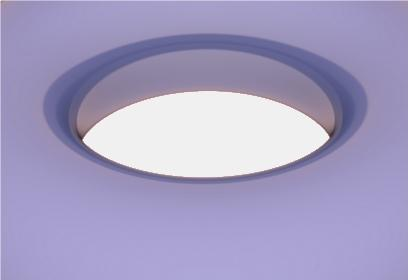
\includegraphics[scale=0.5]{./pictures/C1-torus-step1.jpg}
\end{center}\\
\end{tabular}

\begin{tabular}{m{2.5in} m{2in}}
\pause Ponieważ południki są znacznie krótsze niż równoleżniki, wprowadzamy zaburzenia wzdłuż równoleżników (falowanie).
&\begin{center}
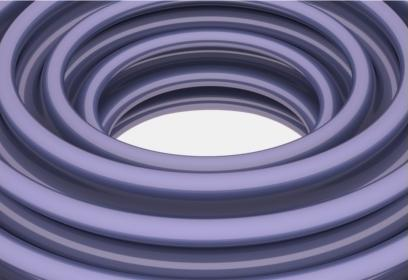
\includegraphics[scale=0.5]{./pictures/C1-torus-step2.jpg}
\end{center}\\
\end{tabular}
\end{frame}

\begin{frame}[plain]

\begin{tabular}{m{2.5in} m{2in}}
Teraz południki są faktycznie dłuższe, ale równoleżniki są (były) różnej długości, więc wprowadzamy drugi poziom falowania (mniejsza amplituda, a większa częstotliwość), aby wyrównać te różnice.
&\pause\begin{center}
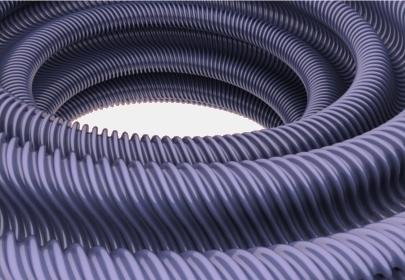
\includegraphics[scale=0.5]{./pictures/C1-torus-step3.jpg}
\end{center}\\
itd... 
\end{tabular}
\end{frame}
\newpage

\begin{frame}[plain]
\mode<presentation>{\hspace*{-0.9in}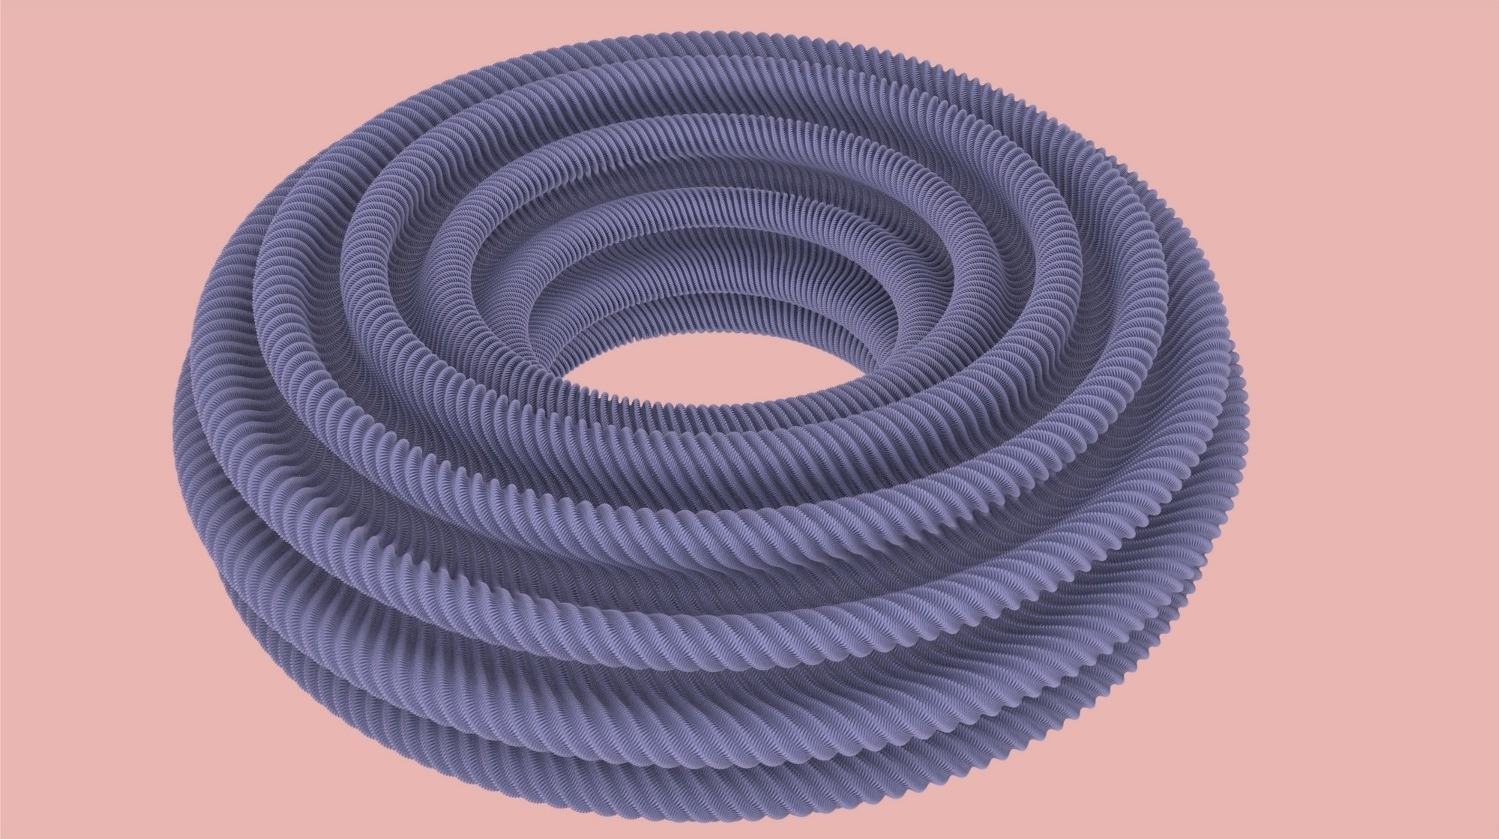
\includegraphics[scale=2]{./pictures/C1-flat-torus-1.png}}
\mode<article>{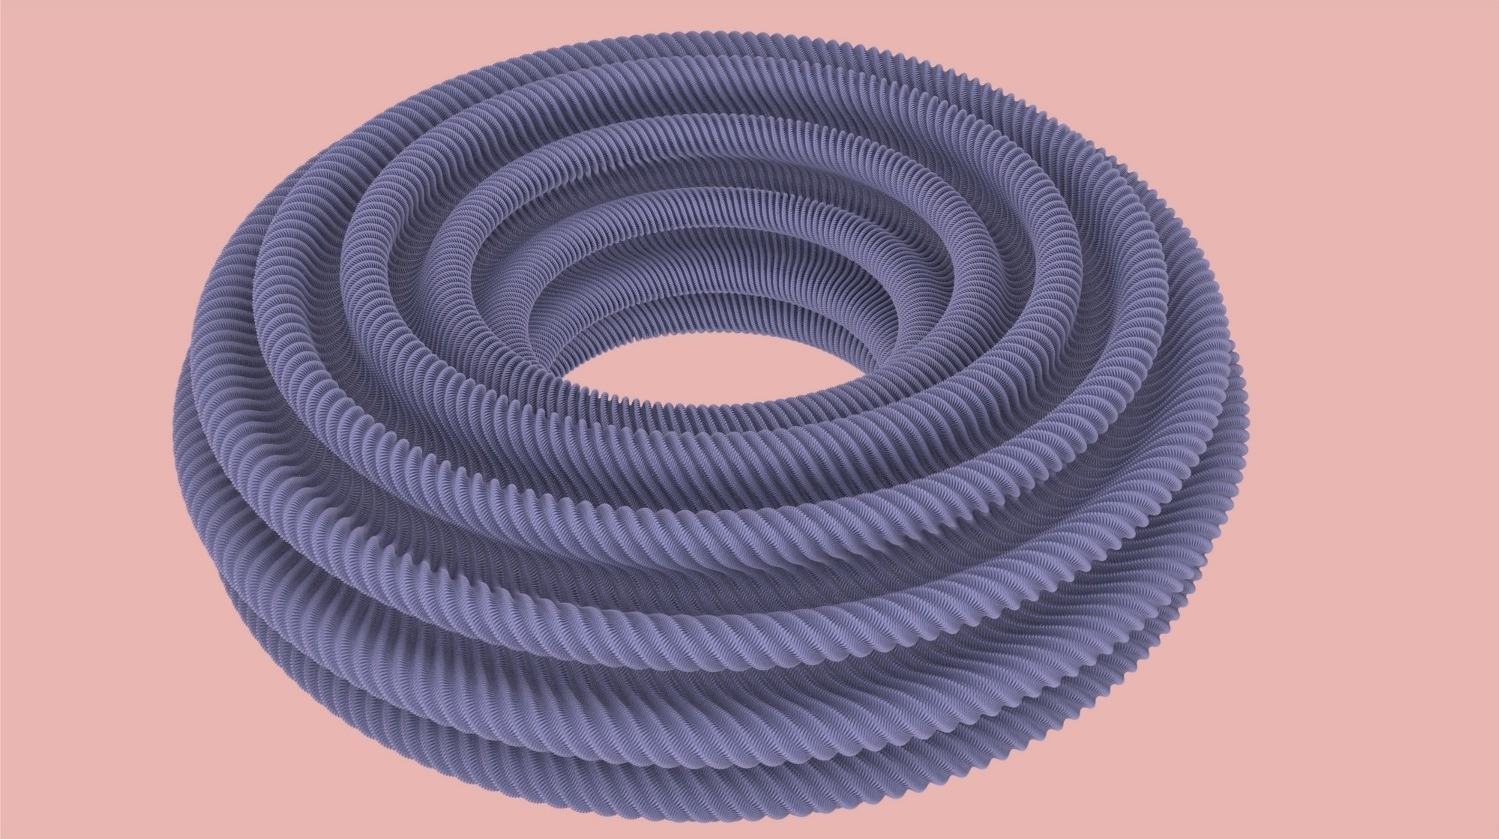
\includegraphics[keepaspectratio=true,width=\textwidth]{./pictures/C1-flat-torus-1.png}}
% \begin{center}
%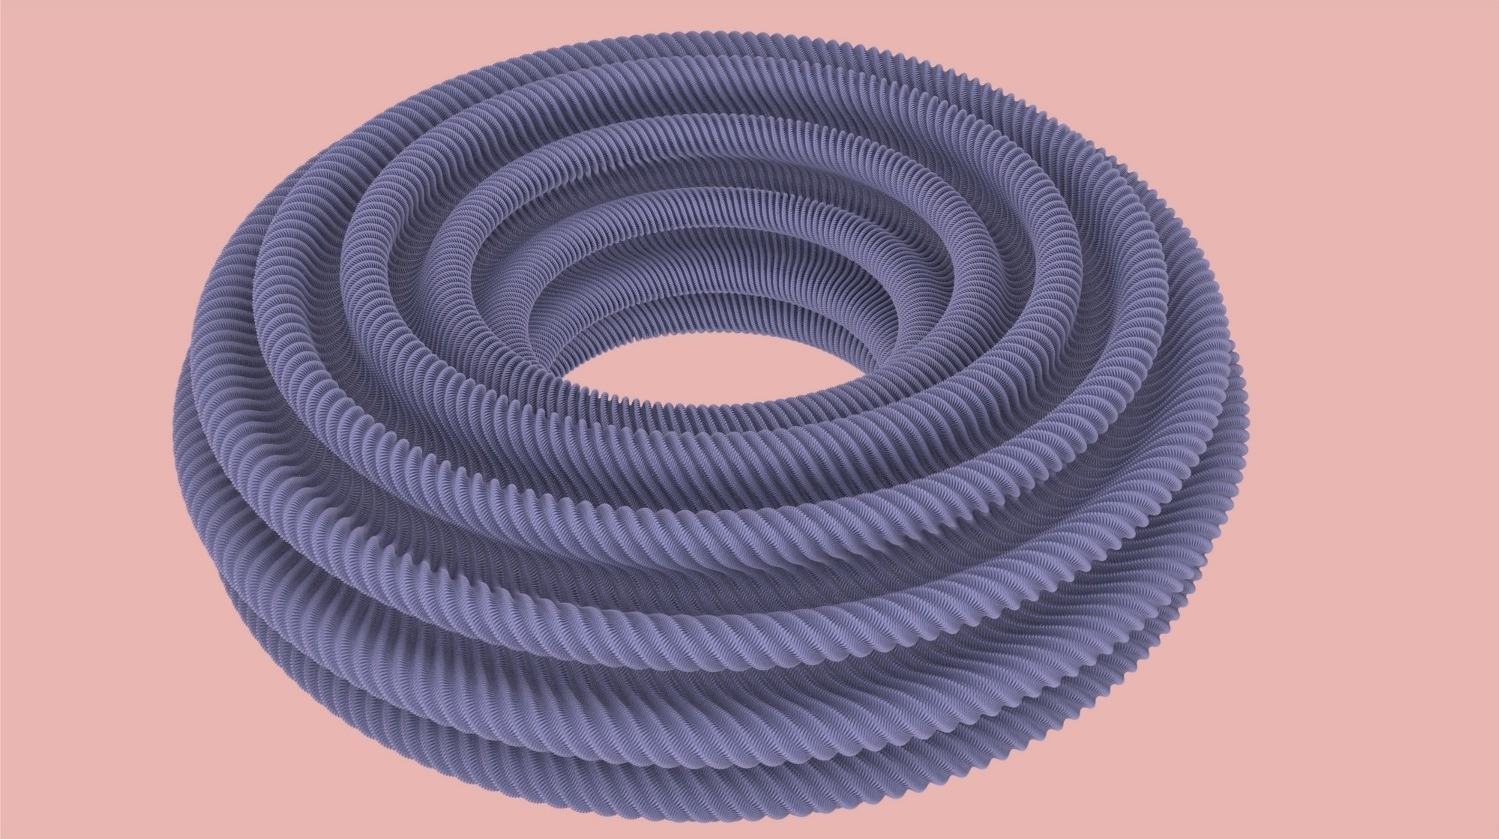
\includegraphics[keepaspectratio=true,width=1\paperwidth]{./pictures/C1-flat-torus-1.png}
% \end{center}
\end{frame}
\smallskip
%\newpage
\begin{frame}[plain]
\mode<presentation>{\hspace*{-0.9in}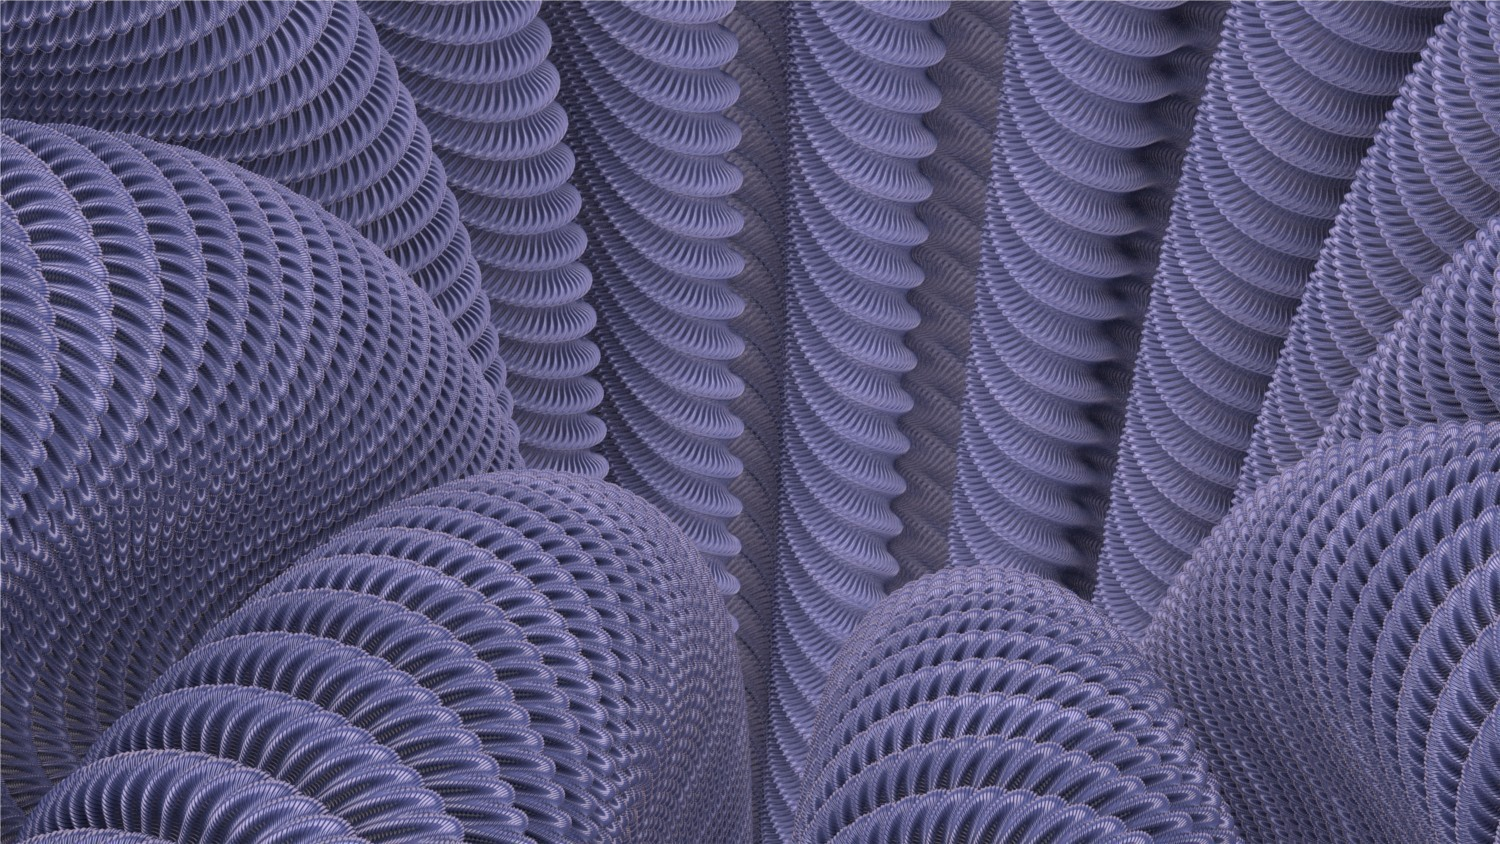
\includegraphics[scale=2]{./pictures/C1-flat-torus-2.png}}
\mode<article>{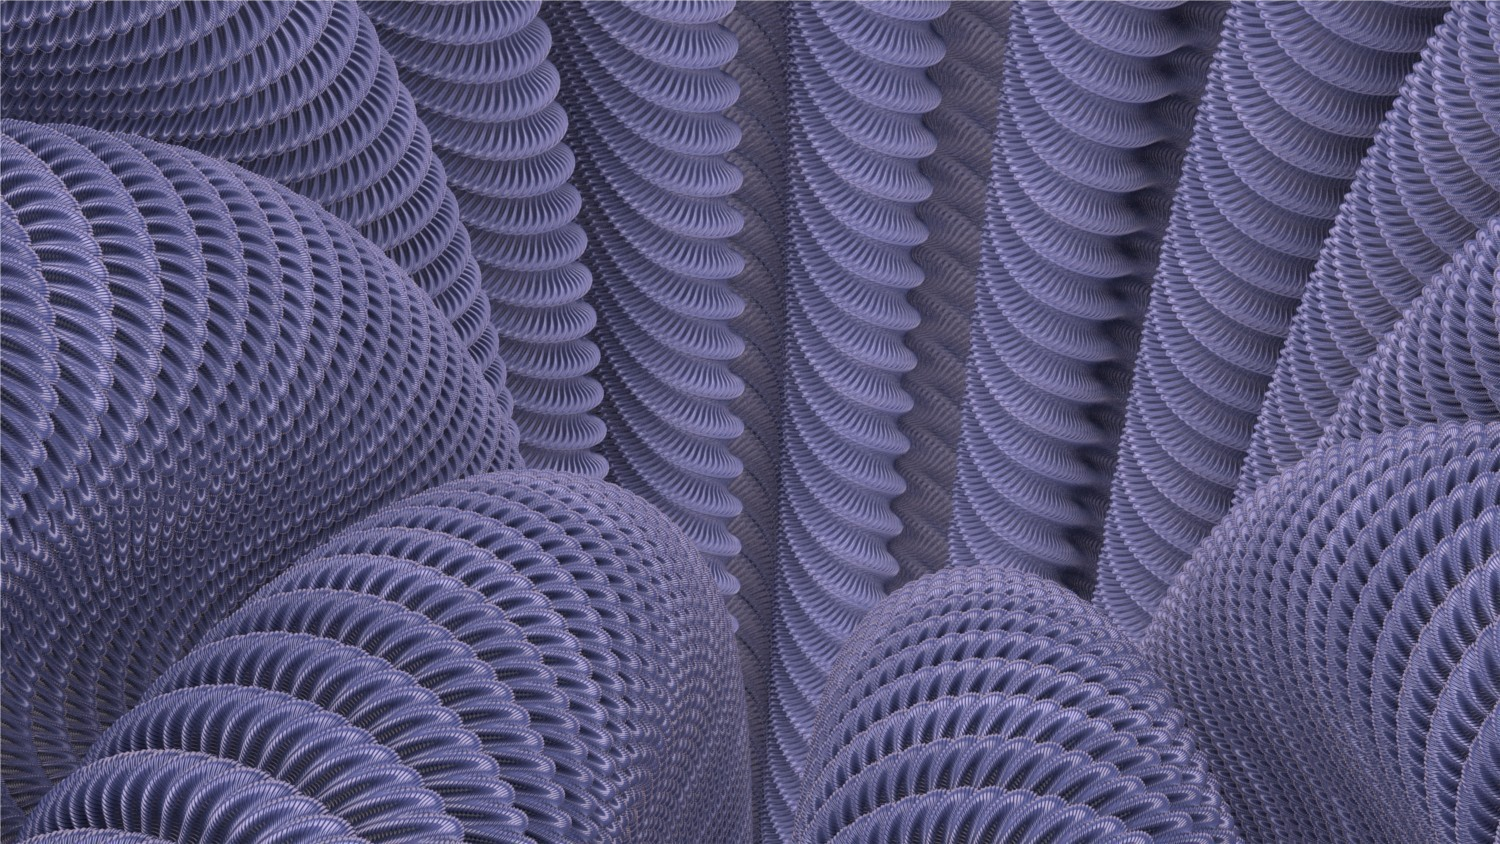
\includegraphics[keepaspectratio=true,width=\textwidth]{./pictures/C1-flat-torus-2.png}}
\end{frame}

%\newpage

\begin{frame}
\begin{itemize}
\item Chociaż wszystkie kroki można wykonać w klasie $C^2$, proces ten 
kontynuujemy w nieskończoność, więc ostateczne zanurzenie jako granica tych 
odwzorowań może być tylko klasy $C^1$.
\mode<article>{
\item Odwzorowanie klasy $C^1$ oznacza, że przestrzeń styczna jest w każdym 
punkcie zdefiniowana, lecz wektor normalny może zdradzać ,,dziwaczne" 
zachowanie (w przypadku tego zanurzenia -- fraktalne).
}
\pause \item Jednocześnie na rysunku poniżej widzimy, że południki i równoleżniki uzyskały tę samą długość.
\begin{center}
\mode<presentation>{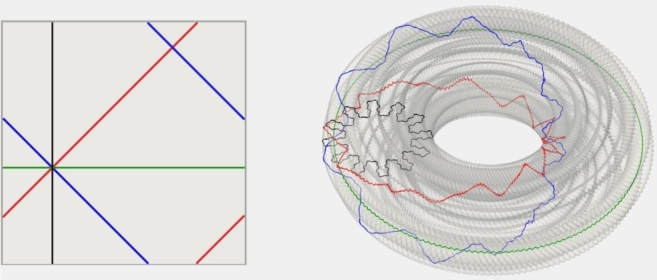
\includegraphics[scale=0.41]{./pictures/C1-flat-torus-equal.jpg}}
\mode<article>{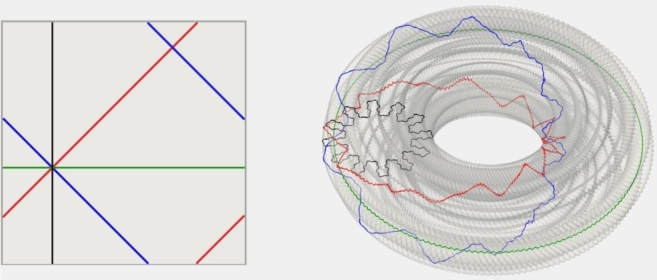
\includegraphics[keepaspectratio=true,width=\textwidth]{./pictures/C1-flat-torus-equal.jpg}}

\end{center}
\end{itemize}
\end{frame}

\begin{frame}[plain]
%\begin{center}
\mode<presentation>{\hspace*{-0.2in}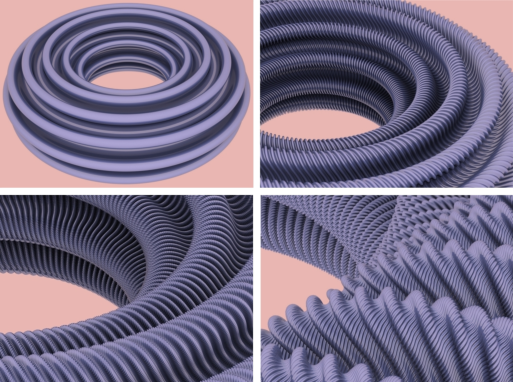
\includegraphics[scale=1.5]{./pictures/flat-torus-1.pdf}}
\mode<article>{\hspace*{0.4in}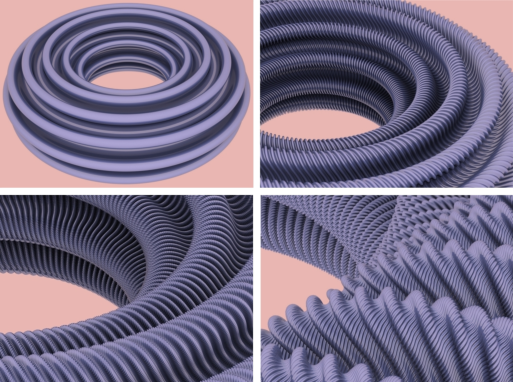
\includegraphics[keepaspectratio=true,width=\textwidth]{./pictures/flat-torus-1.pdf}}

%\end{center}
\end{frame}

% \footnotesize{Rysunki płaskiego zanurzenia torusa w $\R^3$ pochodzą z pracy:\\
% Borrelli, Vincent and Jabrane, Saïd and Lazarus, Francis and Thibert, Boris,
% \textit{Flat tori in three-dimensional space and convex integration}, Proceedings of the National Academy of Sciences, 2012}
\mode<all> 
